\chapter{Vollständige Ergebnisse der Phase 1}
\label{chap:anhang:ergebnisse}

Die Tabellen \ref{tab:anhang:cars} bis \ref{tab:anhang:semiinat} enthalten die Test-\ac{MAP@R} aller Kombinationen aus Verlustfunktion, Verfahren und Budget, jeweils für einzelne Fold-Modelle (Mean) und das Ensemble (Concat). In den Tabellen \ref{tab:anhang:gewinne} und \ref{tab:anhang:klassen} stehen die gepaarten Gewinne aus den Abbildungen \ref{fig:e:gewinne} und \ref{fig:e:klassen} mit ihrer Standardabweichung. Tabelle \ref{tab:anhang:negativ} gibt für die Gewinne aus Abbildung \ref{fig:e:gewinne} die Zahl der gepaarten Vergleiche mit negativer Differenz an. Tabelle \ref{tab:anhang:metriken} stellt die Gewinne in \ac{MAP@R}, \ac{RP} und \ac{P@1} gegenüber. Die Tabellen \ref{tab:cars:hpo} bis \ref{tab:semiinat:hpo} führen die für die Wiederholungen übernommenen Konfigurationen auf. Tabelle \ref{tab:anhang:aufwand} enthält die gemessene Rechenzeit dieser Konfigurationen (Abschnitt \ref{sec:m:aufwand}). Abbildung \ref{fig:e:uebersicht} zeigt die gepaarten Gewinne über das Budget zusammen mit ihrer Spanne über die Verlustfunktionen, Abbildung \ref{fig:e:verluste} je Verlustfunktion beim kleinsten Budget. 

\begin{table}[p]
\centering
\caption[Test-MAP@R Cars196]{Test-MAP@R in \% auf Cars196, Mittel $\pm$ Standardabweichung über fünf Seeds. M: einzelne Fold-Modelle (Mean), C: Ensemble (Concat). Fett: bester Mittelwert je Verlustfunktion, Budget und Modelltyp; zusätzlich unterstrichen: bester Mittelwert je Budget und Modelltyp.}
\label{tab:anhang:cars}
\footnotesize\setlength{\tabcolsep}{4pt}
\begin{tabular}{@{}llS[table-format=2.2(3), retain-zero-uncertainty]S[table-format=2.2(3), retain-zero-uncertainty]S[table-format=2.2(3), retain-zero-uncertainty]S[table-format=2.2(3), retain-zero-uncertainty]S[table-format=2.2(3), retain-zero-uncertainty]@{}}
\toprule
Verfahren & Modell & {ArcFace} & {Circle} & {MS} & {NT-Xent} & {Proxy-Anchor} \\
\midrule
\multicolumn{7}{@{}l}{$k=4$} \\
\addlinespace[2pt]
\UEBL & M & 32.28 +- 0.24 & 32.36 +- 0.28 & 34.26 +- 0.26 & 32.55 +- 0.26 & 31.60 +- 0.25 \\
 & C & 34.52 +- 0.28 & 34.34 +- 0.42 & 36.50 +- 0.23 & 34.62 +- 0.26 & 34.51 +- 0.42 \\
\addlinespace[1pt]
LP & M & \bfseries 38.27 +- 0.26 & \bfseries 41.13 +- 0.14 & {\bfseries\ULdepth=1.5pt\uline{\mbox{\tablenum[table-format=2.2(3), retain-zero-uncertainty]{41.51 +- 0.45}}}} & \bfseries 40.40 +- 0.21 & \bfseries 40.50 +- 0.29 \\
 & C & \bfseries 42.26 +- 0.29 & \bfseries 44.29 +- 0.27 & {\bfseries\ULdepth=1.5pt\uline{\mbox{\tablenum[table-format=2.2(3), retain-zero-uncertainty]{45.63 +- 0.23}}}} & \bfseries 43.86 +- 0.11 & \bfseries 43.61 +- 0.33 \\
\addlinespace[1pt]
LRML & M & 32.93 +- 0.87 & 33.34 +- 0.25 & 33.66 +- 0.19 & 32.91 +- 0.30 & 34.22 +- 0.78 \\
 & C & 36.55 +- 1.19 & 38.56 +- 0.33 & 39.33 +- 0.23 & 39.14 +- 0.66 & 38.09 +- 1.03 \\
\addlinespace[1pt]
Hoffer & M & 34.49 +- 0.24 & 36.61 +- 0.31 & 37.37 +- 0.17 & 35.34 +- 0.89 & 32.56 +- 0.19 \\
 & C & 37.30 +- 0.35 & 41.52 +- 0.30 & 41.33 +- 0.23 & 38.84 +- 0.95 & 34.67 +- 0.22 \\
\addlinespace[1pt]
SLADE & M & 32.32 +- 0.32 & 35.91 +- 0.33 & 35.41 +- 0.40 & 35.47 +- 0.23 & 33.72 +- 0.36 \\
 & C & 35.71 +- 0.47 & 40.36 +- 0.47 & 40.76 +- 0.55 & 39.44 +- 0.39 & 36.25 +- 0.47 \\
\midrule
\multicolumn{7}{@{}l}{$k=8$} \\
\addlinespace[2pt]
\UEBL & M & 37.24 +- 0.24 & 36.70 +- 0.26 & 38.61 +- 0.36 & 36.93 +- 0.29 & 36.31 +- 0.22 \\
 & C & 40.49 +- 0.21 & 39.55 +- 0.25 & 41.64 +- 0.31 & 40.03 +- 0.16 & 40.04 +- 0.27 \\
\addlinespace[1pt]
LP & M & \bfseries 40.64 +- 0.37 & \bfseries 42.23 +- 0.15 & {\bfseries\ULdepth=1.5pt\uline{\mbox{\tablenum[table-format=2.2(3), retain-zero-uncertainty]{42.63 +- 0.10}}}} & \bfseries 41.19 +- 0.07 & \bfseries 42.15 +- 0.16 \\
 & C & \bfseries 43.91 +- 0.31 & \bfseries 45.06 +- 0.11 & {\bfseries\ULdepth=1.5pt\uline{\mbox{\tablenum[table-format=2.2(3), retain-zero-uncertainty]{46.15 +- 0.17}}}} & \bfseries 44.39 +- 0.09 & \bfseries 45.00 +- 0.13 \\
\addlinespace[1pt]
LRML & M & 38.43 +- 0.40 & 38.83 +- 0.47 & 37.89 +- 0.39 & 36.37 +- 0.45 & 40.15 +- 0.33 \\
 & C & 42.97 +- 0.28 & 43.76 +- 0.35 & 43.73 +- 0.35 & 42.88 +- 0.44 & 44.11 +- 0.27 \\
\addlinespace[1pt]
Hoffer & M & 38.33 +- 0.21 & 39.54 +- 0.14 & 39.22 +- 0.08 & 39.42 +- 0.09 & 37.62 +- 0.18 \\
 & C & 42.20 +- 0.23 & 44.15 +- 0.21 & 43.63 +- 0.19 & 43.25 +- 0.19 & 40.98 +- 0.20 \\
\addlinespace[1pt]
SLADE & M & 37.86 +- 0.26 & 39.61 +- 0.23 & 39.67 +- 0.29 & 38.85 +- 0.17 & 38.53 +- 0.27 \\
 & C & 41.06 +- 0.28 & 44.18 +- 0.30 & 44.17 +- 0.38 & 43.28 +- 0.39 & 41.52 +- 0.18 \\
\midrule
\multicolumn{7}{@{}l}{$k=16$} \\
\addlinespace[2pt]
\UEBL & M & 40.67 +- 0.23 & 39.48 +- 0.23 & 41.34 +- 0.34 & 39.55 +- 0.23 & 39.63 +- 0.28 \\
 & C & 43.80 +- 0.25 & 42.86 +- 0.19 & 44.49 +- 0.22 & 42.97 +- 0.25 & 43.38 +- 0.33 \\
\addlinespace[1pt]
LP & M & \bfseries 41.57 +- 0.27 & \bfseries 42.61 +- 0.18 & {\bfseries\ULdepth=1.5pt\uline{\mbox{\tablenum[table-format=2.2(3), retain-zero-uncertainty]{43.25 +- 0.21}}}} & \bfseries 41.64 +- 0.20 & \bfseries 42.72 +- 0.12 \\
 & C & 44.40 +- 0.19 & 45.06 +- 0.21 & {\bfseries\ULdepth=1.5pt\uline{\mbox{\tablenum[table-format=2.2(3), retain-zero-uncertainty]{46.34 +- 0.11}}}} & 44.43 +- 0.12 & 45.19 +- 0.12 \\
\addlinespace[1pt]
LRML & M & 41.14 +- 0.19 & 41.11 +- 0.25 & 40.68 +- 0.37 & 40.22 +- 0.26 & 41.94 +- 0.18 \\
 & C & \bfseries 44.76 +- 0.25 & 44.85 +- 0.24 & 45.37 +- 0.21 & 44.42 +- 0.27 & \bfseries 45.35 +- 0.12 \\
\addlinespace[1pt]
Hoffer & M & 40.58 +- 0.11 & 40.66 +- 0.13 & 39.76 +- 0.19 & 40.72 +- 0.26 & 40.84 +- 0.17 \\
 & C & 44.50 +- 0.22 & 44.60 +- 0.19 & 43.77 +- 0.20 & \bfseries 44.62 +- 0.23 & 44.31 +- 0.21 \\
\addlinespace[1pt]
SLADE & M & 40.67 +- 0.35 & 41.77 +- 0.22 & 42.00 +- 0.37 & 40.78 +- 0.12 & 40.73 +- 0.21 \\
 & C & 43.84 +- 0.26 & \bfseries 45.21 +- 0.27 & 45.31 +- 0.26 & 44.48 +- 0.25 & 43.95 +- 0.22 \\
\midrule
\multicolumn{7}{@{}l}{$k=32$} \\
\addlinespace[2pt]
\UEBL & M & 42.13 +- 0.15 & 41.05 +- 0.30 & 43.00 +- 0.28 & 40.93 +- 0.23 & 41.18 +- 0.23 \\
 & C & 45.02 +- 0.16 & 44.43 +- 0.27 & 45.86 +- 0.24 & 44.22 +- 0.20 & 44.62 +- 0.23 \\
\addlinespace[1pt]
LP & M & 41.84 +- 0.07 & 42.62 +- 0.13 & {\bfseries\ULdepth=1.5pt\uline{\mbox{\tablenum[table-format=2.2(3), retain-zero-uncertainty]{43.42 +- 0.21}}}} & 41.81 +- 0.18 & \bfseries 42.96 +- 0.21 \\
 & C & 44.54 +- 0.07 & 45.13 +- 0.17 & {\bfseries\ULdepth=1.5pt\uline{\mbox{\tablenum[table-format=2.2(3), retain-zero-uncertainty]{46.44 +- 0.11}}}} & 44.54 +- 0.08 & 45.30 +- 0.08 \\
\addlinespace[1pt]
LRML & M & \bfseries 43.05 +- 0.13 & 42.28 +- 0.32 & 43.03 +- 0.24 & \bfseries 42.38 +- 0.22 & 42.11 +- 0.19 \\
 & C & \bfseries 45.54 +- 0.20 & 45.20 +- 0.21 & 46.32 +- 0.17 & \bfseries 45.20 +- 0.16 & 45.07 +- 0.22 \\
\addlinespace[1pt]
Hoffer & M & 41.64 +- 0.18 & 41.16 +- 0.18 & 40.17 +- 0.10 & 41.33 +- 0.18 & 42.56 +- 0.21 \\
 & C & 44.96 +- 0.11 & 44.47 +- 0.16 & 43.59 +- 0.07 & 44.77 +- 0.12 & \bfseries 45.35 +- 0.19 \\
\addlinespace[1pt]
SLADE & M & 41.68 +- 0.28 & \bfseries 42.97 +- 0.24 & 42.96 +- 0.12 & 41.84 +- 0.31 & 41.48 +- 0.30 \\
 & C & 44.57 +- 0.18 & \bfseries 45.69 +- 0.20 & 45.72 +- 0.07 & 44.85 +- 0.16 & 44.55 +- 0.25 \\
\bottomrule
\end{tabular}
\end{table}

\begin{table}[p]
\centering
\caption[Test-MAP@R CUB]{Test-MAP@R in \% auf CUB, Mittel $\pm$ Standardabweichung über fünf Seeds. M: einzelne Fold-Modelle (Mean), C: Ensemble (Concat). Fett: bester Mittelwert je Verlustfunktion, Budget und Modelltyp. Zusätzlich unterstrichen: bester Mittelwert je Budget und Modelltyp.}
\label{tab:anhang:cub}
\footnotesize\setlength{\tabcolsep}{4pt}
\begin{tabular}{@{}llS[table-format=2.2(3), retain-zero-uncertainty]S[table-format=2.2(3), retain-zero-uncertainty]S[table-format=2.2(3), retain-zero-uncertainty]S[table-format=2.2(3), retain-zero-uncertainty]S[table-format=2.2(3), retain-zero-uncertainty]@{}}
\toprule
Verfahren & Modell & {ArcFace} & {Circle} & {MS} & {NT-Xent} & {Proxy-Anchor} \\
\midrule
\multicolumn{7}{@{}l}{$k=4$} \\
\addlinespace[2pt]
\UEBL & M & 51.59 +- 0.10 & 51.67 +- 0.13 & 51.84 +- 0.08 & 51.53 +- 0.12 & \bfseries 51.85 +- 0.10 \\
 & C & 52.23 +- 0.17 & 52.14 +- 0.14 & 52.49 +- 0.13 & 51.94 +- 0.15 & 52.40 +- 0.13 \\
\addlinespace[1pt]
LP & M & 50.96 +- 0.23 & \bfseries 52.29 +- 0.11 & {\bfseries\ULdepth=1.5pt\uline{\mbox{\tablenum[table-format=2.2(3), retain-zero-uncertainty]{52.41 +- 0.12}}}} & \bfseries 52.12 +- 0.16 & 51.79 +- 0.08 \\
 & C & \bfseries 52.76 +- 0.23 & \bfseries 52.85 +- 0.12 & {\bfseries\ULdepth=1.5pt\uline{\mbox{\tablenum[table-format=2.2(3), retain-zero-uncertainty]{53.28 +- 0.16}}}} & 52.67 +- 0.14 & 52.81 +- 0.12 \\
\addlinespace[1pt]
LRML & M & 51.36 +- 0.11 & 50.82 +- 0.24 & 50.50 +- 0.17 & 51.09 +- 0.14 & 51.32 +- 0.18 \\
 & C & 52.53 +- 0.11 & 52.44 +- 0.13 & 52.70 +- 0.15 & \bfseries 52.82 +- 0.09 & \bfseries 53.08 +- 0.05 \\
\addlinespace[1pt]
Hoffer & M & \bfseries 51.66 +- 0.10 & 50.77 +- 0.19 & 51.30 +- 0.18 & 51.66 +- 0.15 & 51.26 +- 0.06 \\
 & C & 52.75 +- 0.10 & 52.53 +- 0.13 & 52.53 +- 0.11 & 52.11 +- 0.16 & 52.83 +- 0.06 \\
\addlinespace[1pt]
SLADE & M & 51.26 +- 0.11 & 51.52 +- 0.10 & 51.64 +- 0.08 & 51.27 +- 0.08 & 51.18 +- 0.23 \\
 & C & 52.24 +- 0.12 & 52.36 +- 0.14 & 52.90 +- 0.18 & 52.42 +- 0.09 & 52.54 +- 0.03 \\
\midrule
\multicolumn{7}{@{}l}{$k=8$} \\
\addlinespace[2pt]
\UEBL & M & \bfseries 51.86 +- 0.15 & 51.97 +- 0.11 & 52.15 +- 0.14 & 51.77 +- 0.13 & \bfseries 52.09 +- 0.15 \\
 & C & 52.64 +- 0.22 & 52.58 +- 0.14 & 52.90 +- 0.20 & 52.28 +- 0.16 & 52.82 +- 0.19 \\
\addlinespace[1pt]
LP & M & 51.06 +- 0.12 & \bfseries 52.46 +- 0.07 & {\bfseries\ULdepth=1.5pt\uline{\mbox{\tablenum[table-format=2.2(3), retain-zero-uncertainty]{52.66 +- 0.08}}}} & \bfseries 52.39 +- 0.09 & 52.02 +- 0.19 \\
 & C & 52.86 +- 0.11 & \bfseries 52.94 +- 0.07 & {\bfseries\ULdepth=1.5pt\uline{\mbox{\tablenum[table-format=2.2(3), retain-zero-uncertainty]{53.36 +- 0.13}}}} & 52.91 +- 0.13 & 52.95 +- 0.12 \\
\addlinespace[1pt]
LRML & M & 51.45 +- 0.24 & 51.60 +- 0.16 & 51.48 +- 0.15 & 51.27 +- 0.17 & 51.57 +- 0.13 \\
 & C & \bfseries 52.95 +- 0.26 & 52.87 +- 0.20 & 53.09 +- 0.26 & \bfseries 52.98 +- 0.21 & \bfseries 53.34 +- 0.11 \\
\addlinespace[1pt]
Hoffer & M & 51.55 +- 0.12 & 51.61 +- 0.25 & 51.91 +- 0.15 & 51.83 +- 0.12 & 51.61 +- 0.12 \\
 & C & 52.93 +- 0.20 & 52.77 +- 0.19 & 52.83 +- 0.18 & 52.43 +- 0.18 & 53.20 +- 0.16 \\
\addlinespace[1pt]
SLADE & M & 51.14 +- 0.15 & 51.95 +- 0.14 & 52.02 +- 0.17 & 51.42 +- 0.11 & 51.82 +- 0.16 \\
 & C & 52.73 +- 0.24 & 52.71 +- 0.17 & 52.96 +- 0.18 & 52.68 +- 0.16 & 52.99 +- 0.17 \\
\midrule
\multicolumn{7}{@{}l}{$k=16$} \\
\addlinespace[2pt]
\UEBL & M & \bfseries 51.90 +- 0.12 & 52.13 +- 0.19 & 52.36 +- 0.14 & 51.89 +- 0.13 & \bfseries 52.12 +- 0.16 \\
 & C & 52.90 +- 0.07 & 52.81 +- 0.09 & 53.21 +- 0.18 & 52.46 +- 0.13 & 52.96 +- 0.08 \\
\addlinespace[1pt]
LP & M & 51.04 +- 0.25 & \bfseries 52.46 +- 0.11 & {\bfseries\ULdepth=1.5pt\uline{\mbox{\tablenum[table-format=2.2(3), retain-zero-uncertainty]{52.79 +- 0.08}}}} & \bfseries 52.52 +- 0.08 & 52.10 +- 0.14 \\
 & C & 52.90 +- 0.13 & 52.93 +- 0.13 & {\bfseries\ULdepth=1.5pt\uline{\mbox{\tablenum[table-format=2.2(3), retain-zero-uncertainty]{53.50 +- 0.05}}}} & \bfseries 53.07 +- 0.09 & 52.94 +- 0.14 \\
\addlinespace[1pt]
LRML & M & 51.82 +- 0.22 & 52.19 +- 0.28 & 52.38 +- 0.14 & 51.79 +- 0.21 & 51.87 +- 0.29 \\
 & C & \bfseries 53.06 +- 0.07 & \bfseries 53.08 +- 0.19 & 53.24 +- 0.13 & 52.99 +- 0.15 & \bfseries 53.34 +- 0.15 \\
\addlinespace[1pt]
Hoffer & M & 51.73 +- 0.16 & 52.01 +- 0.27 & 52.19 +- 0.20 & 51.85 +- 0.19 & 51.91 +- 0.05 \\
 & C & 52.96 +- 0.05 & 52.83 +- 0.11 & 52.95 +- 0.15 & 52.66 +- 0.09 & 53.23 +- 0.06 \\
\addlinespace[1pt]
SLADE & M & 51.49 +- 0.06 & 52.13 +- 0.11 & 52.24 +- 0.19 & 51.84 +- 0.11 & 52.12 +- 0.12 \\
 & C & 52.96 +- 0.14 & 52.89 +- 0.17 & 53.05 +- 0.10 & 52.77 +- 0.09 & 53.11 +- 0.04 \\
\midrule
\multicolumn{7}{@{}l}{$k=32$} \\
\addlinespace[2pt]
\UEBL & M & 52.01 +- 0.11 & 52.27 +- 0.18 & 52.70 +- 0.06 & 52.00 +- 0.11 & 52.08 +- 0.16 \\
 & C & 53.00 +- 0.09 & 52.98 +- 0.07 & 53.51 +- 0.05 & 52.69 +- 0.16 & 52.98 +- 0.09 \\
\addlinespace[1pt]
LP & M & 51.26 +- 0.22 & \bfseries 52.51 +- 0.10 & {\bfseries\ULdepth=1.5pt\uline{\mbox{\tablenum[table-format=2.2(3), retain-zero-uncertainty]{52.93 +- 0.05}}}} & \bfseries 52.60 +- 0.10 & 51.94 +- 0.15 \\
 & C & 53.08 +- 0.17 & 52.86 +- 0.10 & {\bfseries\ULdepth=1.5pt\uline{\mbox{\tablenum[table-format=2.2(3), retain-zero-uncertainty]{53.69 +- 0.06}}}} & \bfseries 53.15 +- 0.10 & 52.80 +- 0.05 \\
\addlinespace[1pt]
LRML & M & \bfseries 52.32 +- 0.06 & 52.49 +- 0.17 & 52.83 +- 0.10 & 52.03 +- 0.25 & 52.04 +- 0.29 \\
 & C & \bfseries 53.23 +- 0.09 & \bfseries 53.20 +- 0.12 & 53.37 +- 0.06 & 53.01 +- 0.12 & \bfseries 53.23 +- 0.14 \\
\addlinespace[1pt]
Hoffer & M & 52.13 +- 0.06 & 52.17 +- 0.23 & 52.49 +- 0.11 & 51.89 +- 0.13 & 52.11 +- 0.13 \\
 & C & 53.01 +- 0.06 & 52.89 +- 0.06 & 53.10 +- 0.07 & 52.71 +- 0.09 & 53.17 +- 0.09 \\
\addlinespace[1pt]
SLADE & M & 51.98 +- 0.12 & 52.31 +- 0.16 & 52.31 +- 0.07 & 52.18 +- 0.09 & \bfseries 52.37 +- 0.08 \\
 & C & 53.10 +- 0.12 & 53.00 +- 0.07 & 53.05 +- 0.17 & 52.90 +- 0.05 & 53.07 +- 0.07 \\
\bottomrule
\end{tabular}
\end{table}

\begin{table}[p]
\centering
\caption[Test-MAP@R In-Shop]{Test-MAP@R in \% auf In-Shop, Mittel $\pm$ Standardabweichung über fünf Seeds. M: einzelne Fold-Modelle (Mean), C: Ensemble (Concat). Fett: bester Mittelwert je Verlustfunktion, Budget und Modelltyp. Zusätzlich unterstrichen: bester Mittelwert je Budget und Modelltyp.}
\label{tab:anhang:inshop}
\footnotesize\setlength{\tabcolsep}{4pt}
\begin{tabular}{@{}llS[table-format=2.2(3), retain-zero-uncertainty]S[table-format=2.2(3), retain-zero-uncertainty]S[table-format=2.2(3), retain-zero-uncertainty]S[table-format=2.2(3), retain-zero-uncertainty]S[table-format=2.2(3), retain-zero-uncertainty]@{}}
\toprule
Verfahren & Modell & {ArcFace} & {Circle} & {MS} & {NT-Xent} & {Proxy-Anchor} \\
\midrule
\multicolumn{7}{@{}l}{$k=2$} \\
\addlinespace[2pt]
\UEBL & M & 54.67 +- 0.13 & 54.52 +- 0.12 & 55.91 +- 0.16 & 54.45 +- 0.10 & 53.70 +- 0.13 \\
 & C & 57.35 +- 0.08 & 57.54 +- 0.22 & 58.79 +- 0.14 & 57.24 +- 0.10 & 55.98 +- 0.13 \\
\addlinespace[1pt]
LP & M & {\bfseries\ULdepth=1.5pt\uline{\mbox{\tablenum[table-format=2.2(3), retain-zero-uncertainty]{58.90 +- 0.05}}}} & 57.62 +- 0.10 & \bfseries 58.76 +- 0.06 & 57.75 +- 0.14 & 56.24 +- 0.15 \\
 & C & \bfseries 60.58 +- 0.05 & 59.85 +- 0.11 & {\bfseries\ULdepth=1.5pt\uline{\mbox{\tablenum[table-format=2.2(3), retain-zero-uncertainty]{61.06 +- 0.15}}}} & 59.94 +- 0.22 & 57.27 +- 0.17 \\
\addlinespace[1pt]
LRML & M & 57.52 +- 0.46 & 57.50 +- 0.12 & 56.30 +- 0.26 & 55.60 +- 0.14 & 53.77 +- 0.24 \\
 & C & 59.67 +- 0.46 & 59.31 +- 0.11 & 59.33 +- 0.25 & 59.31 +- 0.26 & 56.02 +- 0.17 \\
\addlinespace[1pt]
Hoffer & M & 57.69 +- 0.09 & \bfseries 57.89 +- 0.08 & 57.80 +- 0.07 & \bfseries 58.09 +- 0.07 & \bfseries 57.50 +- 0.11 \\
 & C & 60.37 +- 0.13 & \bfseries 60.11 +- 0.09 & 60.71 +- 0.12 & \bfseries 60.54 +- 0.17 & \bfseries 60.10 +- 0.08 \\
\addlinespace[1pt]
SLADE & M & 53.09 +- 0.48 & 54.62 +- 0.13 & 54.37 +- 0.13 & 53.86 +- 0.18 & 53.41 +- 0.30 \\
 & C & 56.33 +- 0.51 & 56.80 +- 0.24 & 57.36 +- 0.23 & 56.70 +- 0.19 & 57.81 +- 0.12 \\
\midrule
\multicolumn{7}{@{}l}{$k=4$} \\
\addlinespace[2pt]
\UEBL & M & \bfseries 59.78 +- 0.06 & 59.52 +- 0.10 & {\bfseries\ULdepth=1.5pt\uline{\mbox{\tablenum[table-format=2.2(3), retain-zero-uncertainty]{60.55 +- 0.17}}}} & 58.95 +- 0.10 & 57.18 +- 0.05 \\
 & C & 61.13 +- 0.09 & 61.02 +- 0.16 & 61.64 +- 0.19 & 60.12 +- 0.11 & 58.31 +- 0.07 \\
\addlinespace[1pt]
LP & M & 59.61 +- 0.07 & 59.53 +- 0.11 & 60.41 +- 0.08 & \bfseries 59.34 +- 0.08 & 56.54 +- 0.13 \\
 & C & \bfseries 61.47 +- 0.07 & \bfseries 61.25 +- 0.15 & {\bfseries\ULdepth=1.5pt\uline{\mbox{\tablenum[table-format=2.2(3), retain-zero-uncertainty]{62.22 +- 0.13}}}} & \bfseries 60.98 +- 0.11 & 57.76 +- 0.12 \\
\addlinespace[1pt]
LRML & M & 58.41 +- 0.31 & 59.36 +- 0.20 & 59.08 +- 0.21 & 57.43 +- 0.14 & 58.08 +- 0.11 \\
 & C & 59.63 +- 0.16 & 60.27 +- 0.24 & 60.48 +- 0.26 & 59.55 +- 0.20 & 59.19 +- 0.16 \\
\addlinespace[1pt]
Hoffer & M & 58.74 +- 0.09 & \bfseries 59.65 +- 0.27 & 59.29 +- 0.10 & 58.95 +- 0.08 & \bfseries 58.59 +- 0.07 \\
 & C & 60.66 +- 0.25 & 61.07 +- 0.29 & 61.42 +- 0.16 & 60.70 +- 0.10 & \bfseries 60.05 +- 0.12 \\
\addlinespace[1pt]
SLADE & M & 59.20 +- 0.21 & 58.75 +- 0.07 & 60.02 +- 0.03 & 59.06 +- 0.06 & 55.61 +- 0.91 \\
 & C & 60.47 +- 0.22 & 59.63 +- 0.13 & 61.33 +- 0.11 & 60.40 +- 0.11 & 57.65 +- 0.86 \\
\bottomrule
\end{tabular}
\end{table}

\begin{table}[p]
\centering
\caption[Test-MAP@R In-Shop mit gelabelten Klassen]{Test-MAP@R in \% auf In-Shop mit gelabelten Klassen, Mittel $\pm$ Standardabweichung über fünf Seeds. M: einzelne Fold-Modelle (Mean), C: Ensemble (Concat). Fett: bester Mittelwert je Verlustfunktion, Budget und Modelltyp; zusätzlich unterstrichen: bester Mittelwert je Budget und Modelltyp. Die großen Standardabweichungen bei LP mit ArcFace bei 25 und 50\,\% entstehen, weil dort einzelne Fold-Modelle deutlich schlechter sind.}
\label{tab:anhang:inshop10}
\footnotesize\setlength{\tabcolsep}{4pt}
\begin{tabular}{@{}llS[table-format=2.2(3), retain-zero-uncertainty]S[table-format=2.2(3), retain-zero-uncertainty]S[table-format=2.2(3), retain-zero-uncertainty]S[table-format=2.2(3), retain-zero-uncertainty]S[table-format=2.2(3), retain-zero-uncertainty]@{}}
\toprule
Verfahren & Modell & {ArcFace} & {Circle} & {MS} & {NT-Xent} & {Proxy-Anchor} \\
\midrule
\multicolumn{7}{@{}l}{5\,\%} \\
\addlinespace[2pt]
\UEBL & M & 43.39 +- 0.13 & 43.02 +- 0.12 & 43.20 +- 0.19 & \bfseries 43.37 +- 0.16 & \bfseries 43.19 +- 0.21 \\
 & C & 47.75 +- 0.35 & 47.48 +- 0.17 & 47.85 +- 0.32 & \bfseries 47.43 +- 0.17 & 47.39 +- 0.29 \\
\addlinespace[1pt]
LP & M & 39.49 +- 0.32 & 42.37 +- 0.23 & \bfseries 43.70 +- 0.24 & 42.99 +- 0.12 & 39.77 +- 0.23 \\
 & C & 46.24 +- 0.25 & 47.03 +- 0.27 & 47.15 +- 0.23 & 46.97 +- 0.20 & 43.72 +- 0.15 \\
\addlinespace[1pt]
LRML & M & 43.39 +- 0.11 & {\bfseries\ULdepth=1.5pt\uline{\mbox{\tablenum[table-format=2.2(3), retain-zero-uncertainty]{45.24 +- 0.28}}}} & 43.42 +- 0.26 & 42.50 +- 0.19 & 41.23 +- 0.27 \\
 & C & \bfseries 48.47 +- 0.20 & {\bfseries\ULdepth=1.5pt\uline{\mbox{\tablenum[table-format=2.2(3), retain-zero-uncertainty]{50.89 +- 0.45}}}} & \bfseries 50.33 +- 0.42 & 47.20 +- 0.07 & \bfseries 47.58 +- 0.34 \\
\addlinespace[1pt]
Hoffer & M & \bfseries 43.75 +- 0.14 & 43.00 +- 0.16 & 43.29 +- 0.17 & 43.17 +- 0.14 & 42.70 +- 0.22 \\
 & C & 48.01 +- 0.10 & 47.65 +- 0.17 & 48.01 +- 0.26 & 47.38 +- 0.16 & 46.08 +- 0.18 \\
\addlinespace[1pt]
SLADE & M & 43.63 +- 0.18 & 43.32 +- 0.16 & 43.53 +- 0.21 & 43.31 +- 0.10 & 42.59 +- 0.28 \\
 & C & 47.89 +- 0.24 & 47.19 +- 0.18 & 48.10 +- 0.23 & 47.29 +- 0.07 & 46.79 +- 0.37 \\
\midrule
\multicolumn{7}{@{}l}{10\,\%} \\
\addlinespace[2pt]
\UEBL & M & 48.39 +- 0.17 & 47.80 +- 0.18 & 48.55 +- 0.12 & \bfseries 48.17 +- 0.15 & \bfseries 48.11 +- 0.10 \\
 & C & 52.58 +- 0.26 & 52.14 +- 0.14 & 52.89 +- 0.28 & 51.87 +- 0.15 & \bfseries 51.84 +- 0.14 \\
\addlinespace[1pt]
LP & M & 45.63 +- 0.04 & 47.05 +- 0.25 & 48.39 +- 0.19 & 47.95 +- 0.12 & 44.57 +- 0.21 \\
 & C & 51.49 +- 0.06 & 50.58 +- 0.27 & 51.64 +- 0.30 & 51.20 +- 0.12 & 47.59 +- 0.28 \\
\addlinespace[1pt]
LRML & M & 48.41 +- 0.30 & {\bfseries\ULdepth=1.5pt\uline{\mbox{\tablenum[table-format=2.2(3), retain-zero-uncertainty]{50.74 +- 0.06}}}} & \bfseries 49.03 +- 0.17 & 46.91 +- 0.16 & 47.25 +- 0.19 \\
 & C & \bfseries 52.79 +- 0.34 & {\bfseries\ULdepth=1.5pt\uline{\mbox{\tablenum[table-format=2.2(3), retain-zero-uncertainty]{55.42 +- 0.14}}}} & \bfseries 54.33 +- 0.39 & 51.64 +- 0.21 & 51.57 +- 0.14 \\
\addlinespace[1pt]
Hoffer & M & \bfseries 48.80 +- 0.13 & 47.75 +- 0.21 & 48.38 +- 0.14 & 48.04 +- 0.18 & 47.33 +- 0.13 \\
 & C & 52.72 +- 0.31 & 52.25 +- 0.13 & 52.72 +- 0.18 & \bfseries 51.97 +- 0.19 & 50.45 +- 0.17 \\
\addlinespace[1pt]
SLADE & M & 48.45 +- 0.13 & 48.09 +- 0.20 & 48.41 +- 0.16 & 48.10 +- 0.13 & 44.42 +- 2.16 \\
 & C & 51.94 +- 0.24 & 51.64 +- 0.30 & 52.13 +- 0.28 & 51.81 +- 0.35 & 48.83 +- 2.32 \\
\midrule
\multicolumn{7}{@{}l}{25\,\%} \\
\addlinespace[2pt]
\UEBL & M & 54.61 +- 0.11 & 53.67 +- 0.15 & \bfseries 55.14 +- 0.12 & 53.91 +- 0.20 & \bfseries 53.87 +- 0.16 \\
 & C & \bfseries 58.13 +- 0.19 & 57.29 +- 0.23 & 58.00 +- 0.27 & 56.62 +- 0.25 & \bfseries 56.76 +- 0.20 \\
\addlinespace[1pt]
LP & M & 46.81 +- 2.30 & 50.85 +- 0.08 & 53.09 +- 0.12 & 53.04 +- 0.13 & 48.55 +- 0.25 \\
 & C & 55.23 +- 0.39 & 53.14 +- 0.16 & 55.54 +- 0.16 & 55.75 +- 0.25 & 50.51 +- 0.24 \\
\addlinespace[1pt]
LRML & M & 52.67 +- 1.13 & {\bfseries\ULdepth=1.5pt\uline{\mbox{\tablenum[table-format=2.2(3), retain-zero-uncertainty]{55.75 +- 0.26}}}} & 53.83 +- 0.16 & 52.53 +- 0.11 & 51.26 +- 0.36 \\
 & C & 55.92 +- 1.52 & {\bfseries\ULdepth=1.5pt\uline{\mbox{\tablenum[table-format=2.2(3), retain-zero-uncertainty]{58.55 +- 0.35}}}} & 57.50 +- 0.20 & 56.46 +- 0.18 & 53.29 +- 0.34 \\
\addlinespace[1pt]
Hoffer & M & \bfseries 55.14 +- 0.09 & 53.46 +- 0.18 & 55.07 +- 0.17 & \bfseries 54.14 +- 0.18 & 52.96 +- 0.12 \\
 & C & 58.07 +- 0.07 & 57.19 +- 0.27 & \bfseries 58.13 +- 0.31 & \bfseries 57.16 +- 0.29 & 55.32 +- 0.20 \\
\addlinespace[1pt]
SLADE & M & 53.99 +- 0.20 & 53.59 +- 0.13 & 54.03 +- 0.10 & 53.36 +- 0.16 & 45.88 +- 0.89 \\
 & C & 56.29 +- 0.17 & 56.37 +- 0.20 & 56.22 +- 0.19 & 56.25 +- 0.16 & 49.59 +- 1.55 \\
\midrule
\multicolumn{7}{@{}l}{50\,\%} \\
\addlinespace[2pt]
\UEBL & M & 58.23 +- 0.07 & 56.81 +- 0.14 & 58.48 +- 0.13 & 56.78 +- 0.20 & \bfseries 57.30 +- 0.10 \\
 & C & {\bfseries\ULdepth=1.5pt\uline{\mbox{\tablenum[table-format=2.2(3), retain-zero-uncertainty]{60.49 +- 0.14}}}} & 59.10 +- 0.16 & 60.00 +- 0.15 & 58.25 +- 0.23 & \bfseries 59.13 +- 0.08 \\
\addlinespace[1pt]
LP & M & 49.19 +- 5.35 & 53.08 +- 0.42 & 55.20 +- 0.20 & 55.95 +- 0.05 & 50.36 +- 0.12 \\
 & C & 54.71 +- 0.79 & 55.77 +- 1.23 & 56.88 +- 0.23 & 58.14 +- 0.13 & 52.19 +- 0.21 \\
\addlinespace[1pt]
LRML & M & 55.84 +- 0.54 & \bfseries 57.81 +- 0.32 & 55.09 +- 0.20 & 55.60 +- 0.21 & 52.02 +- 0.38 \\
 & C & 58.46 +- 0.42 & \bfseries 59.58 +- 0.36 & 57.66 +- 0.27 & 58.29 +- 0.22 & 53.05 +- 0.30 \\
\addlinespace[1pt]
Hoffer & M & {\bfseries\ULdepth=1.5pt\uline{\mbox{\tablenum[table-format=2.2(3), retain-zero-uncertainty]{58.71 +- 0.06}}}} & 56.64 +- 0.07 & \bfseries 58.70 +- 0.12 & \bfseries 57.42 +- 0.13 & 56.11 +- 0.27 \\
 & C & 60.37 +- 0.12 & 59.15 +- 0.10 & \bfseries 60.44 +- 0.15 & \bfseries 59.13 +- 0.14 & 57.51 +- 0.29 \\
\addlinespace[1pt]
SLADE & M & 57.68 +- 0.13 & 56.49 +- 0.08 & 56.86 +- 0.17 & 55.86 +- 0.59 & 50.22 +- 1.93 \\
 & C & 59.28 +- 0.24 & 58.20 +- 0.13 & 57.96 +- 0.25 & 58.06 +- 0.79 & 54.03 +- 1.64 \\
\bottomrule
\end{tabular}
\end{table}

\begin{table}[p]
\centering
\caption[Test-MAP@R Semi-iNat-2021]{Test-MAP@R in \% auf Semi-iNat-2021, Mittel $\pm$ Standardabweichung über fünf Seeds. M: einzelne Fold-Modelle (Mean), C: Ensemble (Concat). Fett: bester Mittelwert je Verlustfunktion, Budget und Modelltyp. Zusätzlich unterstrichen: bester Mittelwert je Budget und Modelltyp.}
\label{tab:anhang:semiinat}
\footnotesize\setlength{\tabcolsep}{4pt}
\begin{tabular}{@{}llS[table-format=2.2(3), retain-zero-uncertainty]S[table-format=2.2(3), retain-zero-uncertainty]S[table-format=2.2(3), retain-zero-uncertainty]S[table-format=2.2(3), retain-zero-uncertainty]S[table-format=2.2(3), retain-zero-uncertainty]@{}}
\toprule
Verfahren & Modell & {ArcFace} & {Circle} & {MS} & {NT-Xent} & {Proxy-Anchor} \\
\midrule
\multicolumn{7}{@{}l}{$k=2$} \\
\addlinespace[2pt]
\UEBL & M & 34.11 +- 0.04 & 34.13 +- 0.07 & 34.14 +- 0.06 & 34.08 +- 0.08 & 34.11 +- 0.05 \\
 & C & 34.63 +- 0.03 & 34.60 +- 0.05 & 34.38 +- 0.06 & 34.53 +- 0.05 & 34.63 +- 0.03 \\
\addlinespace[1pt]
LP & M & \bfseries 34.31 +- 0.08 & \bfseries 34.75 +- 0.06 & {\bfseries\ULdepth=1.5pt\uline{\mbox{\tablenum[table-format=2.2(3), retain-zero-uncertainty]{35.14 +- 0.08}}}} & \bfseries 34.72 +- 0.08 & \bfseries 34.41 +- 0.11 \\
 & C & \bfseries 35.31 +- 0.08 & \bfseries 35.81 +- 0.09 & {\bfseries\ULdepth=1.5pt\uline{\mbox{\tablenum[table-format=2.2(3), retain-zero-uncertainty]{35.92 +- 0.10}}}} & \bfseries 35.67 +- 0.09 & \bfseries 35.46 +- 0.09 \\
\addlinespace[1pt]
LRML & M & 34.11 +- 0.06 & 33.97 +- 0.08 & 34.12 +- 0.06 & 34.01 +- 0.06 & 33.99 +- 0.06 \\
 & C & 34.47 +- 0.03 & 34.61 +- 0.08 & 34.42 +- 0.06 & 34.78 +- 0.05 & 34.64 +- 0.05 \\
\addlinespace[1pt]
Hoffer & M & 34.08 +- 0.04 & 34.05 +- 0.07 & 34.12 +- 0.08 & 34.05 +- 0.07 & 34.15 +- 0.06 \\
 & C & 34.71 +- 0.01 & 34.53 +- 0.06 & 34.53 +- 0.06 & 34.46 +- 0.05 & 34.47 +- 0.05 \\
\addlinespace[1pt]
SLADE & M & 34.14 +- 0.07 & 34.07 +- 0.07 & 34.09 +- 0.07 & 34.06 +- 0.08 & 34.15 +- 0.06 \\
 & C & 34.52 +- 0.03 & 34.68 +- 0.07 & 34.38 +- 0.06 & 34.53 +- 0.05 & 34.47 +- 0.02 \\
\midrule
\multicolumn{7}{@{}l}{$k=4$} \\
\addlinespace[2pt]
\UEBL & M & 34.72 +- 0.06 & 34.75 +- 0.08 & 34.81 +- 0.08 & 34.66 +- 0.08 & 34.67 +- 0.09 \\
 & C & 35.50 +- 0.05 & 35.50 +- 0.09 & 35.38 +- 0.08 & 35.25 +- 0.09 & 35.47 +- 0.10 \\
\addlinespace[1pt]
LP & M & \bfseries 35.00 +- 0.05 & \bfseries 35.45 +- 0.08 & {\bfseries\ULdepth=1.5pt\uline{\mbox{\tablenum[table-format=2.2(3), retain-zero-uncertainty]{35.76 +- 0.08}}}} & \bfseries 35.47 +- 0.09 & \bfseries 35.11 +- 0.08 \\
 & C & \bfseries 36.24 +- 0.04 & \bfseries 36.52 +- 0.07 & {\bfseries\ULdepth=1.5pt\uline{\mbox{\tablenum[table-format=2.2(3), retain-zero-uncertainty]{36.65 +- 0.05}}}} & \bfseries 36.56 +- 0.08 & \bfseries 36.27 +- 0.09 \\
\addlinespace[1pt]
LRML & M & 34.72 +- 0.08 & 34.55 +- 0.11 & 34.78 +- 0.09 & 34.43 +- 0.09 & 34.57 +- 0.08 \\
 & C & 35.31 +- 0.08 & 35.51 +- 0.09 & 35.34 +- 0.08 & 35.66 +- 0.09 & 35.48 +- 0.09 \\
\addlinespace[1pt]
Hoffer & M & 34.62 +- 0.05 & 34.68 +- 0.09 & 34.81 +- 0.08 & 34.63 +- 0.10 & 34.76 +- 0.08 \\
 & C & 35.51 +- 0.06 & 35.42 +- 0.10 & 35.47 +- 0.09 & 35.15 +- 0.11 & 35.35 +- 0.08 \\
\addlinespace[1pt]
SLADE & M & 34.70 +- 0.08 & 34.67 +- 0.10 & 34.77 +- 0.09 & 34.63 +- 0.09 & 34.74 +- 0.08 \\
 & C & 35.33 +- 0.10 & 35.57 +- 0.11 & 35.35 +- 0.10 & 35.27 +- 0.10 & 35.32 +- 0.08 \\
\midrule
\multicolumn{7}{@{}l}{$k=16$} \\
\addlinespace[2pt]
\UEBL & M & 36.01 +- 0.07 & 36.05 +- 0.08 & 36.19 +- 0.09 & 36.02 +- 0.07 & 35.67 +- 0.09 \\
 & C & 37.10 +- 0.07 & 37.00 +- 0.11 & 36.97 +- 0.09 & 36.89 +- 0.08 & 36.84 +- 0.09 \\
\addlinespace[1pt]
LP & M & \bfseries 36.02 +- 0.05 & \bfseries 36.45 +- 0.04 & \bfseries 36.64 +- 0.04 & {\bfseries\ULdepth=1.5pt\uline{\mbox{\tablenum[table-format=2.2(3), retain-zero-uncertainty]{36.71 +- 0.05}}}} & \bfseries 36.05 +- 0.06 \\
 & C & \bfseries 37.21 +- 0.03 & \bfseries 37.35 +- 0.04 & \bfseries 37.37 +- 0.03 & {\bfseries\ULdepth=1.5pt\uline{\mbox{\tablenum[table-format=2.2(3), retain-zero-uncertainty]{37.60 +- 0.03}}}} & \bfseries 36.95 +- 0.05 \\
\addlinespace[1pt]
LRML & M & 35.94 +- 0.10 & 35.77 +- 0.09 & 36.26 +- 0.08 & 35.56 +- 0.10 & 35.56 +- 0.10 \\
 & C & 36.89 +- 0.09 & 36.89 +- 0.06 & 37.12 +- 0.08 & 36.54 +- 0.06 & 36.85 +- 0.09 \\
\addlinespace[1pt]
Hoffer & M & 35.82 +- 0.05 & 36.10 +- 0.07 & 36.15 +- 0.08 & 36.06 +- 0.07 & 35.83 +- 0.08 \\
 & C & 37.04 +- 0.06 & 37.09 +- 0.10 & 36.99 +- 0.09 & 36.91 +- 0.07 & 36.77 +- 0.09 \\
\addlinespace[1pt]
SLADE & M & 35.89 +- 0.09 & 35.96 +- 0.11 & 36.25 +- 0.09 & 35.97 +- 0.08 & 35.70 +- 0.09 \\
 & C & 36.87 +- 0.07 & 37.13 +- 0.09 & 37.15 +- 0.10 & 36.88 +- 0.07 & 36.72 +- 0.08 \\
\midrule
\multicolumn{7}{@{}l}{$k=100$} \\
\addlinespace[2pt]
\UEBL & M & \bfseries 37.03 +- 0.02 & 37.15 +- 0.05 & 37.34 +- 0.06 & \bfseries 37.27 +- 0.05 & 36.49 +- 0.04 \\
 & C & \bfseries 37.96 +- 0.02 & 37.85 +- 0.04 & 38.01 +- 0.05 & \bfseries 37.97 +- 0.03 & 37.37 +- 0.04 \\
\addlinespace[1pt]
LP & M & 35.94 +- 0.02 & 36.14 +- 0.05 & 36.31 +- 0.03 & 36.45 +- 0.03 & 36.24 +- 0.03 \\
 & C & 37.09 +- 0.03 & 37.09 +- 0.07 & 37.14 +- 0.05 & 37.38 +- 0.05 & 36.76 +- 0.04 \\
\addlinespace[1pt]
LRML & M & 36.67 +- 0.06 & 36.76 +- 0.04 & {\bfseries\ULdepth=1.5pt\uline{\mbox{\tablenum[table-format=2.2(3), retain-zero-uncertainty]{37.53 +- 0.05}}}} & 35.95 +- 0.05 & 36.28 +- 0.05 \\
 & C & 37.52 +- 0.06 & 37.57 +- 0.03 & {\bfseries\ULdepth=1.5pt\uline{\mbox{\tablenum[table-format=2.2(3), retain-zero-uncertainty]{38.23 +- 0.05}}}} & 36.72 +- 0.04 & 37.38 +- 0.05 \\
\addlinespace[1pt]
Hoffer & M & 36.91 +- 0.03 & \bfseries 37.31 +- 0.04 & 37.13 +- 0.04 & 37.26 +- 0.02 & \bfseries 36.70 +- 0.04 \\
 & C & 37.94 +- 0.01 & \bfseries 38.09 +- 0.02 & 37.89 +- 0.03 & 37.96 +- 0.02 & \bfseries 37.50 +- 0.02 \\
\addlinespace[1pt]
SLADE & M & 36.66 +- 0.05 & 36.69 +- 0.06 & 37.38 +- 0.06 & 37.13 +- 0.06 & 36.08 +- 0.03 \\
 & C & 37.45 +- 0.05 & 37.48 +- 0.06 & 38.12 +- 0.05 & 37.81 +- 0.04 & 36.84 +- 0.04 \\
\bottomrule
\end{tabular}
\end{table}

\begin{table}[tbp]
\centering
\caption[Gewinn der SSL-Verfahren mit Standardabweichung]{Gepaarter Gewinn der Test-MAP@R gegenüber der \UEBL in Prozentpunkten, gemittelt über die fünf Seeds und die fünf Verlustfunktionen, $\pm$ Standardabweichung der 25 gepaarten Differenzen. Sie gibt vor allem die Unterschiede zwischen den Verlustfunktionen wieder, die Seed-Standardabweichung des Mittels liegt bei höchstens 0,4 Prozentpunkten. Fett: größter gerundeter Gewinn je Zeile, getrennt nach Mean und Concat, sofern er positiv ist.}
\label{tab:anhang:gewinne}
\footnotesize\setlength{\tabcolsep}{2pt}
\begin{tabular}{@{}l r@{\hspace{6pt}} *{8}{S[table-format=+1.1(2), retain-explicit-plus, retain-zero-uncertainty]}@{}}
\toprule
 & & \multicolumn{4}{c}{Mean} & \multicolumn{4}{c}{Concat} \\
\cmidrule(lr){3-6}\cmidrule(l){7-10}
{Datensatz} & {$k$} & {LP} & {\acs{LRML}} & {Hoffer} & {SLADE} & {LP} & {\acs{LRML}} & {Hoffer} & {SLADE} \\
\midrule
Cars196 & 4 & \bfseries +7.8 +- 1.1 & +0.8 +- 1.2 & +2.7 +- 1.1 & +2.0 +- 1.3 & \bfseries +9.0 +- 0.8 & +3.4 +- 1.1 & +3.8 +- 2.4 & +3.6 +- 1.9 \\
 & 8 & \bfseries +4.6 +- 1.0 & +1.2 +- 1.8 & +1.7 +- 0.9 & +1.7 +- 0.9 & \bfseries +4.5 +- 0.7 & +3.1 +- 0.9 & +2.5 +- 1.3 & +2.5 +- 1.5 \\
 & 16 & \bfseries +2.2 +- 0.9 & +0.9 +- 1.1 & +0.4 +- 1.1 & +1.1 +- 0.8 & \bfseries +1.6 +- 0.6 & +1.5 +- 0.5 & +0.9 +- 0.9 & +1.1 +- 0.8 \\
 & 32 & \bfseries +0.9 +- 0.8 & \bfseries +0.9 +- 0.5 & -0.3 +- 1.5 & +0.5 +- 0.9 & +0.4 +- 0.5 & \bfseries +0.6 +- 0.3 & -0.2 +- 1.1 & +0.2 +- 0.7 \\
\addlinespace
\acs{CUB} & 4 & \bfseries +0.2 +- 0.5 & -0.7 +- 0.4 & -0.4 +- 0.4 & -0.3 +- 0.2 & \bfseries +0.6 +- 0.2 & +0.5 +- 0.3 & +0.3 +- 0.2 & +0.3 +- 0.2 \\
 & 8 & \bfseries +0.2 +- 0.6 & -0.5 +- 0.2 & -0.3 +- 0.2 & -0.3 +- 0.3 & \bfseries +0.4 +- 0.2 & \bfseries +0.4 +- 0.2 & +0.2 +- 0.2 & +0.2 +- 0.2 \\
 & 16 & \bfseries +0.1 +- 0.6 & -0.1 +- 0.2 & -0.1 +- 0.1 & -0.1 +- 0.2 & +0.2 +- 0.3 & \bfseries +0.3 +- 0.2 & +0.1 +- 0.2 & +0.1 +- 0.2 \\
 & 32 & +0.0 +- 0.5 & \bfseries +0.1 +- 0.2 & -0.1 +- 0.2 & +0.0 +- 0.3 & +0.1 +- 0.3 & \bfseries +0.2 +- 0.2 & -0.1 +- 0.2 & +0.0 +- 0.3 \\
\addlinespace
In-Shop & 2 & \bfseries +3.2 +- 0.6 & +1.5 +- 1.3 & +3.1 +- 0.7 & -0.8 +- 0.7 & +2.4 +- 0.7 & +1.3 +- 0.9 & \bfseries +3.0 +- 0.8 & -0.4 +- 1.2 \\
 & 4 & -0.1 +- 0.4 & -0.7 +- 1.0 & -0.2 +- 1.0 & -0.7 +- 0.7 & \bfseries +0.3 +- 0.5 & -0.6 +- 0.9 & \bfseries +0.3 +- 0.8 & -0.5 +- 0.7 \\
\addlinespace
Semi-iNat & 2 & \bfseries +0.6 +- 0.3 & -0.1 +- 0.1 & +0.0 +- 0.0 & +0.0 +- 0.0 & \bfseries +1.1 +- 0.3 & +0.0 +- 0.1 & +0.0 +- 0.1 & +0.0 +- 0.1 \\
 & 4 & \bfseries +0.6 +- 0.3 & -0.1 +- 0.1 & +0.0 +- 0.1 & +0.0 +- 0.1 & \bfseries +1.0 +- 0.2 & +0.0 +- 0.2 & +0.0 +- 0.1 & -0.1 +- 0.1 \\
 & 16 & \bfseries +0.4 +- 0.2 & -0.2 +- 0.2 & +0.0 +- 0.1 & +0.0 +- 0.1 & \bfseries +0.3 +- 0.2 & -0.1 +- 0.2 & +0.0 +- 0.1 & +0.0 +- 0.2 \\
 & 100 & -0.8 +- 0.3 & -0.4 +- 0.5 & +0.0 +- 0.2 & -0.3 +- 0.2 & -0.7 +- 0.1 & -0.4 +- 0.5 & +0.0 +- 0.1 & -0.3 +- 0.2 \\
\bottomrule
\end{tabular}
\end{table}

\begin{table}[tbp]
\centering
\caption[Gewinn bei vollständig gelabelten Klassen mit Standardabweichung]{In-Shop mit vollständig gelabelten Klassen: Test-MAP@R der \UEBL in \% und gepaarter Gewinn der \acs{SSL}-Verfahren in Prozentpunkten, Mittel über die fünf Seeds und die fünf Verlustfunktionen, beim Gewinn $\pm$ Standardabweichung der 25 gepaarten Differenzen. Anteil: vollständig gelabelte Trainingsklassen. Fett: größter Gewinn je Spalte, sofern er positiv ist. M: Mean, C: Concat.}
\label{tab:anhang:klassen}
\footnotesize\setlength{\tabcolsep}{2pt}
\begin{tabular}{@{}l *{8}{S[table-format=+1.1(2), retain-explicit-plus, retain-zero-uncertainty]}@{}}
\toprule
{Anteil} & \multicolumn{2}{c}{\qty{5}{\percent}} & \multicolumn{2}{c}{\qty{10}{\percent}} & \multicolumn{2}{c}{\qty{25}{\percent}} & \multicolumn{2}{c}{\qty{50}{\percent}} \\
\cmidrule(lr){2-3}\cmidrule(lr){4-5}\cmidrule(lr){6-7}\cmidrule(lr){8-9}
 & {M} & {C} & {M} & {C} & {M} & {C} & {M} & {C} \\
\midrule
\multicolumn{9}{@{}l}{\emph{Test-MAP@R der \UEBL in \%}} \\
\UEBL & {43,2} & {47,6} & {48,2} & {52,3} & {54,2} & {57,4} & {57,5} & {59,4} \\
\addlinespace
\multicolumn{9}{@{}l}{\emph{Gewinn}} \\
LP & -1.6 +- 1.8 & -1.4 +- 1.3 & -1.5 +- 1.4 & -1.8 +- 1.3 & -3.8 +- 2.7 & -3.3 +- 1.9 & -4.8 +- 3.7 & -3.9 +- 2.5 \\
\acs{LRML} & -0.1 +- 1.4 & \bfseries +1.3 +- 1.5 & \bfseries +0.3 +- 1.5 & \bfseries +0.9 +- 1.4 & -1.0 +- 1.7 & -1.0 +- 1.8 & -2.2 +- 2.2 & -2.0 +- 2.4 \\
Hoffer & -0.1 +- 0.3 & -0.2 +- 0.6 & -0.1 +- 0.4 & -0.2 +- 0.6 & -0.1 +- 0.5 & -0.2 +- 0.7 & +0.0 +- 0.7 & -0.1 +- 0.9 \\
SLADE & +0.0 +- 0.4 & -0.1 +- 0.4 & -0.7 +- 1.8 & -1.0 +- 1.4 & -2.1 +- 3.1 & -2.4 +- 2.6 & -2.1 +- 2.7 & -1.9 +- 1.9 \\
\bottomrule
\end{tabular}
\end{table}

\clearpage %
\begin{figure}[tbp]
  \centering
  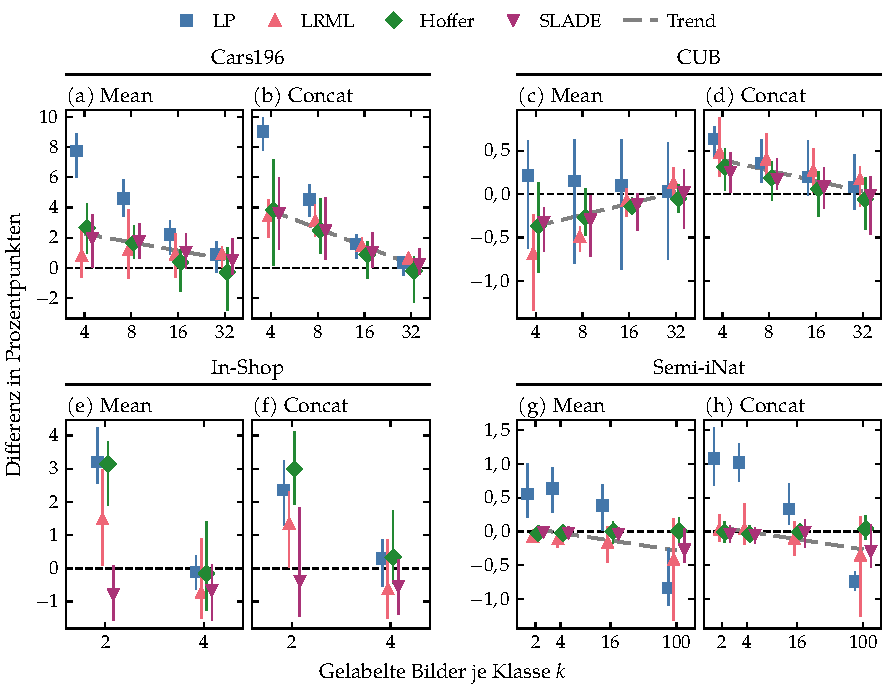
\includegraphics{neu/phase1_uebersicht}
  \caption[Gewinn der \acs{SSL}-Verfahren über das Label-Budget]{Gepaarter Gewinn der Test-\acs{MAP@R} der vier \acs{SSL}-Verfahren gegenüber der \UEBL, Mittel über die fünf Verlustfunktionen (Punkte) mit ihrer Spanne (senkrechte Striche). Grau gestrichelt: Trend über die vier Verfahren (lineare Anpassung an ihren Median je Budget), auf In-Shop mit nur zwei Budgets keiner. Je Datensatz links Mean, rechts Concat, die $y$-Achse ist je Datensatz anders skaliert.}
  \label{fig:e:uebersicht}
\end{figure}

\begin{figure}[tbp]
  \centering
  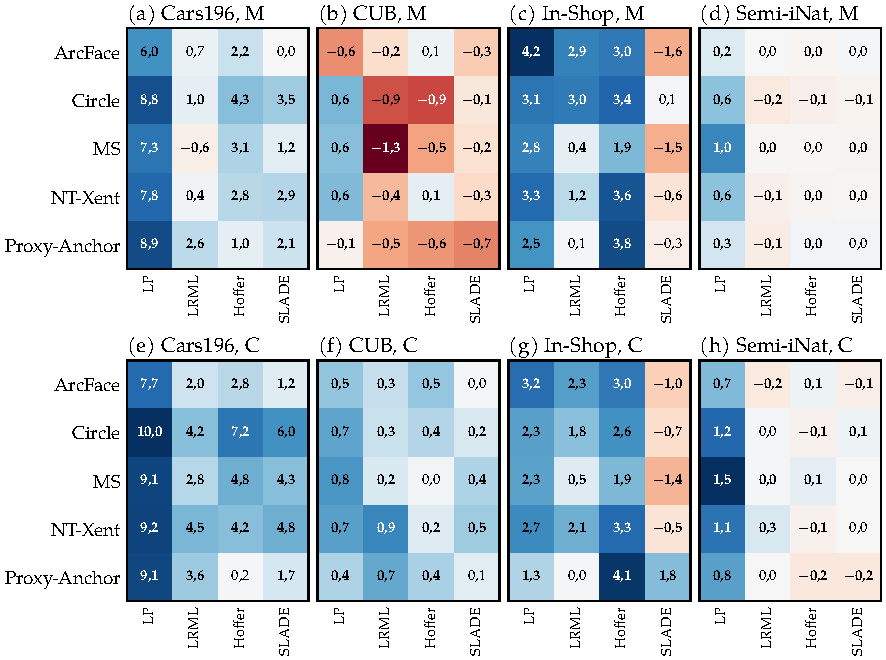
\includegraphics{neu/phase1_verluste}
  \caption[Gewinn je Verlustfunktion und Verfahren beim kleinsten Budget]{Gepaarter Gewinn der Test-\acs{MAP@R} je Verlustfunktion und Verfahren beim kleinsten Budget (Cars196 und \acs{CUB}: $k=4$, In-Shop und Semi-iNat-2021: $k=2$). (a) bis (d): Mean (M), (e) bis (h): Concat (C). Fett: Vorzeichen in allen fünf Seeds gleich. Farbskala je Datensatz symmetrisch um null.}
  \label{fig:e:verluste}
\end{figure}

\begin{table}[tbp]
\centering
\caption[Negative Vergleiche gegenüber der supervised Referenz]{Zahl der gepaarten Vergleiche (von 25), in denen ein \acs{SSL}-Verfahren eine niedrigere Test-MAP@R erreichte als die \UEBL, zu den Gewinnen in Tabelle \ref{tab:anhang:gewinne}. M: Mean, C: Concat.}
\label{tab:anhang:negativ}
\small
\begin{tabular}{@{}l *{8}{S[table-format=2.0]}@{}}
\toprule
\multicolumn{9}{@{}l}{\emph{Cars196}} \\
 & \multicolumn{2}{c}{$k=4$} & \multicolumn{2}{c}{$k=8$} & \multicolumn{2}{c}{$k=16$} & \multicolumn{2}{c}{$k=32$} \\
\cmidrule(lr){2-3}\cmidrule(lr){4-5}\cmidrule(lr){6-7}\cmidrule(lr){8-9}
 & {M} & {C} & {M} & {C} & {M} & {C} & {M} & {C} \\
LP & 0 & 0 & 0 & 0 & 0 & 0 & 5 & 5 \\
\acs{LRML} & 6 & 0 & 10 & 0 & 5 & 0 & 1 & 0 \\
Hoffer & 0 & 3 & 0 & 0 & 8 & 5 & 12 & 11 \\
SLADE & 2 & 0 & 0 & 0 & 3 & 2 & 11 & 13 \\
\midrule
\multicolumn{9}{@{}l}{\emph{\acs{CUB}}} \\
 & \multicolumn{2}{c}{$k=4$} & \multicolumn{2}{c}{$k=8$} & \multicolumn{2}{c}{$k=16$} & \multicolumn{2}{c}{$k=32$} \\
\cmidrule(lr){2-3}\cmidrule(lr){4-5}\cmidrule(lr){6-7}\cmidrule(lr){8-9}
 & {M} & {C} & {M} & {C} & {M} & {C} & {M} & {C} \\
LP & 10 & 0 & 9 & 2 & 7 & 5 & 10 & 12 \\
\acs{LRML} & 25 & 0 & 25 & 0 & 14 & 2 & 6 & 5 \\
Hoffer & 16 & 1 & 19 & 5 & 21 & 8 & 17 & 14 \\
SLADE & 25 & 4 & 22 & 3 & 15 & 7 & 10 & 10 \\
\midrule
\multicolumn{9}{@{}l}{\emph{In-Shop}} \\
 & \multicolumn{2}{c}{$k=2$} & \multicolumn{2}{c}{$k=4$} & {} & {} & {} & {} \\
\cmidrule(lr){2-3}\cmidrule(lr){4-5}
 & {M} & {C} & {M} & {C} & {} & {} & {} & {} \\
LP & 0 & 0 & 17 & 5 & {} & {} & {} & {} \\
\acs{LRML} & 3 & 3 & 19 & 20 & {} & {} & {} & {} \\
Hoffer & 0 & 0 & 14 & 12 & {} & {} & {} & {} \\
SLADE & 20 & 20 & 21 & 18 & {} & {} & {} & {} \\
\midrule
\multicolumn{9}{@{}l}{\emph{Semi-iNat-2021}} \\
 & \multicolumn{2}{c}{$k=2$} & \multicolumn{2}{c}{$k=4$} & \multicolumn{2}{c}{$k=16$} & \multicolumn{2}{c}{$k=100$} \\
\cmidrule(lr){2-3}\cmidrule(lr){4-5}\cmidrule(lr){6-7}\cmidrule(lr){8-9}
 & {M} & {C} & {M} & {C} & {M} & {C} & {M} & {C} \\
LP & 0 & 0 & 0 & 0 & 0 & 0 & 25 & 25 \\
\acs{LRML} & 23 & 8 & 23 & 14 & 19 & 17 & 20 & 17 \\
Hoffer & 19 & 15 & 17 & 18 & 10 & 16 & 14 & 11 \\
SLADE & 17 & 16 & 19 & 15 & 15 & 13 & 20 & 20 \\
\bottomrule
\end{tabular}
\end{table}

\begin{table}[tbp]
\centering
\caption[Gewinn der \acs{SSL}-Verfahren in \acs{MAP@R}, \acs{RP} und \acs{P@1}]{Gepaarter Gewinn der \acs{SSL}-Verfahren gegenüber der \UEBL in \acs{MAP@R}, \acs{RP} und \acs{P@1} in Prozentpunkten, gemittelt über die fünf Seeds und die fünf Verlustfunktionen. M: einzelne Fold-Modelle (Mean), C: Ensemble (Concat). In-Shop-Serie: Anteil vollständig gelabelter Klassen. Fett: größter gerundeter Gewinn je Zeile und Metrik, sofern er positiv ist.}
\label{tab:anhang:metriken}
\footnotesize\setlength{\tabcolsep}{2pt}
\begin{tabular}{@{}l r c@{\hspace{4pt}} *{12}{S[table-format=+1.1, retain-explicit-plus]}@{}}
\toprule
 & &  & \multicolumn{3}{c}{LP} & \multicolumn{3}{c}{\acs{LRML}} & \multicolumn{3}{c}{Hoffer} & \multicolumn{3}{c}{SLADE} \\
\cmidrule(lr){4-6}\cmidrule(lr){7-9}\cmidrule(lr){10-12}\cmidrule(l){13-15}
{Datensatz} & {Budget} &  & {\acs{MAP@R}} & {\acs{RP}} & {\acs{P@1}} & {\acs{MAP@R}} & {\acs{RP}} & {\acs{P@1}} & {\acs{MAP@R}} & {\acs{RP}} & {\acs{P@1}} & {\acs{MAP@R}} & {\acs{RP}} & {\acs{P@1}} \\
\midrule
Cars196 & 4 & M & \bfseries +7.8 & \bfseries +6.7 & \bfseries +3.4 & +0.8 & +0.5 & +0.1 & +2.7 & +2.1 & +1.5 & +2.0 & +1.3 & +1.1 \\
 &  & C & \bfseries +9.0 & \bfseries +7.4 & \bfseries +4.8 & +3.4 & +2.7 & +2.0 & +3.8 & +2.9 & +2.3 & +3.6 & +2.6 & +2.5 \\
 & 8 & M & \bfseries +4.6 & \bfseries +4.1 & \bfseries +1.2 & +1.2 & +1.1 & -0.4 & +1.7 & +1.3 & +0.4 & +1.7 & +1.4 & +0.7 \\
 &  & C & \bfseries +4.5 & \bfseries +3.7 & \bfseries +1.9 & +3.1 & +2.6 & +1.5 & +2.5 & +1.8 & +1.2 & +2.5 & +1.8 & +1.5 \\
 & 16 & M & \bfseries +2.2 & \bfseries +2.0 & \bfseries +0.1 & +0.9 & +1.0 & -0.6 & +0.4 & +0.3 & -0.7 & +1.1 & +0.8 & \bfseries +0.1 \\
 &  & C & \bfseries +1.6 & \bfseries +1.3 & +0.2 & +1.5 & +1.2 & +0.4 & +0.9 & +0.6 & +0.0 & +1.1 & +0.7 & \bfseries +0.5 \\
 & 32 & M & \bfseries +0.9 & +0.8 & +0.0 & \bfseries +0.9 & \bfseries +0.9 & +0.0 & -0.3 & -0.3 & -1.0 & +0.5 & +0.4 & \bfseries +0.2 \\
 &  & C & +0.4 & +0.3 & -0.2 & \bfseries +0.6 & \bfseries +0.6 & +0.0 & -0.2 & -0.3 & -0.6 & +0.2 & +0.1 & +0.0 \\
\addlinespace
\acs{CUB} & 4 & M & \bfseries +0.2 & \bfseries +0.2 & -0.2 & -0.7 & -0.6 & -0.6 & -0.4 & -0.3 & -0.4 & -0.3 & -0.3 & -0.3 \\
 &  & C & \bfseries +0.6 & \bfseries +0.6 & \bfseries +0.1 & +0.5 & +0.4 & +0.0 & +0.3 & +0.2 & +0.0 & +0.3 & +0.2 & \bfseries +0.1 \\
 & 8 & M & \bfseries +0.2 & \bfseries +0.2 & -0.2 & -0.5 & -0.4 & -0.5 & -0.3 & -0.2 & -0.3 & -0.3 & -0.3 & -0.2 \\
 &  & C & \bfseries +0.4 & \bfseries +0.3 & -0.1 & \bfseries +0.4 & \bfseries +0.3 & -0.1 & +0.2 & +0.2 & -0.1 & +0.2 & +0.1 & +0.0 \\
 & 16 & M & \bfseries +0.1 & \bfseries +0.1 & -0.1 & -0.1 & +0.0 & -0.1 & -0.1 & -0.1 & -0.1 & -0.1 & -0.1 & +0.0 \\
 &  & C & +0.2 & \bfseries +0.2 & +0.0 & \bfseries +0.3 & \bfseries +0.2 & \bfseries +0.1 & +0.1 & +0.0 & +0.0 & +0.1 & +0.1 & \bfseries +0.1 \\
 & 32 & M & +0.0 & \bfseries +0.1 & +0.0 & \bfseries +0.1 & \bfseries +0.1 & +0.0 & -0.1 & +0.0 & -0.1 & +0.0 & +0.0 & \bfseries +0.1 \\
 &  & C & +0.1 & +0.1 & +0.1 & \bfseries +0.2 & \bfseries +0.2 & +0.1 & -0.1 & -0.1 & +0.0 & +0.0 & +0.0 & \bfseries +0.2 \\
\addlinespace
In-Shop & 2 & M & \bfseries +3.2 & \bfseries +2.9 & \bfseries +2.5 & +1.5 & +1.3 & +1.3 & +3.1 & +2.8 & +1.9 & -0.8 & -0.7 & -0.8 \\
 &  & C & +2.4 & +2.1 & \bfseries +1.7 & +1.3 & +1.1 & +1.2 & \bfseries +3.0 & \bfseries +2.7 & \bfseries +1.7 & -0.4 & -0.3 & -0.4 \\
 & 4 & M & -0.1 & -0.1 & -0.7 & -0.7 & -0.7 & -0.4 & -0.2 & -0.2 & -1.1 & -0.7 & -0.6 & -0.7 \\
 &  & C & \bfseries +0.3 & \bfseries +0.3 & -0.5 & -0.6 & -0.6 & -0.3 & \bfseries +0.3 & \bfseries +0.3 & -0.8 & -0.5 & -0.5 & -0.6 \\
\addlinespace
In-Shop-Serie & 5\,\% & M & -1.6 & -1.5 & -1.9 & -0.1 & -0.2 & -0.3 & -0.1 & -0.1 & +0.0 & +0.0 & +0.0 & \bfseries +0.1 \\
 &  & C & -1.4 & -1.4 & -1.5 & \bfseries +1.3 & \bfseries +1.1 & \bfseries +1.0 & -0.2 & -0.1 & -0.1 & -0.1 & -0.2 & -0.1 \\
 & 10\,\% & M & -1.5 & -1.4 & -1.7 & \bfseries +0.3 & \bfseries +0.2 & +0.0 & -0.1 & -0.1 & -0.1 & -0.7 & -0.7 & -0.7 \\
 &  & C & -1.8 & -1.7 & -1.8 & \bfseries +0.9 & \bfseries +0.7 & \bfseries +0.6 & -0.2 & -0.2 & -0.3 & -1.0 & -1.0 & -0.9 \\
 & 25\,\% & M & -3.8 & -3.6 & -3.5 & -1.0 & -1.0 & -1.1 & -0.1 & -0.1 & +0.0 & -2.1 & -2.0 & -1.8 \\
 &  & C & -3.3 & -3.1 & -2.9 & -1.0 & -1.0 & -0.9 & -0.2 & -0.2 & -0.1 & -2.4 & -2.3 & -2.0 \\
 & 50\,\% & M & -4.8 & -4.5 & -4.2 & -2.2 & -2.1 & -2.1 & +0.0 & +0.0 & +0.0 & -2.1 & -2.0 & -1.7 \\
 &  & C & -3.9 & -3.6 & -3.2 & -2.0 & -1.9 & -1.8 & -0.1 & +0.0 & -0.1 & -1.9 & -1.8 & -1.6 \\
\addlinespace
Semi-iNat & 2 & M & \bfseries +0.6 & \bfseries +0.6 & \bfseries +0.1 & -0.1 & -0.1 & +0.0 & +0.0 & +0.0 & +0.0 & +0.0 & +0.0 & +0.0 \\
 &  & C & \bfseries +1.1 & \bfseries +1.1 & \bfseries +0.3 & +0.0 & +0.0 & +0.0 & +0.0 & +0.0 & +0.0 & +0.0 & +0.0 & +0.0 \\
 & 4 & M & \bfseries +0.6 & \bfseries +0.7 & \bfseries +0.1 & -0.1 & -0.1 & -0.1 & +0.0 & +0.0 & +0.0 & +0.0 & +0.0 & +0.0 \\
 &  & C & \bfseries +1.0 & \bfseries +1.0 & \bfseries +0.3 & +0.0 & +0.0 & +0.0 & +0.0 & +0.0 & +0.0 & -0.1 & +0.0 & +0.0 \\
 & 16 & M & \bfseries +0.4 & \bfseries +0.4 & \bfseries +0.1 & -0.2 & -0.2 & -0.1 & +0.0 & +0.0 & +0.0 & +0.0 & +0.0 & +0.0 \\
 &  & C & \bfseries +0.3 & \bfseries +0.3 & \bfseries +0.1 & -0.1 & -0.1 & -0.1 & +0.0 & +0.0 & +0.0 & +0.0 & +0.0 & +0.0 \\
 & 100 & M & -0.8 & -0.9 & -0.4 & -0.4 & -0.4 & -0.2 & +0.0 & +0.0 & +0.0 & -0.3 & -0.2 & -0.1 \\
 &  & C & -0.7 & -0.8 & -0.3 & -0.4 & -0.4 & -0.2 & +0.0 & +0.0 & +0.0 & -0.3 & -0.3 & -0.1 \\
\bottomrule
\end{tabular}
\end{table}

\clearpage
\begin{table}[htbp]
\centering
\caption[Übernommene Konfigurationen Cars196]{Für die Wiederholungen übernommene HPO-Konfigurationen (Optimierung bei $k=16$, Seed~7). Versuch: Nummer innerhalb der Suche, $B$: supervised bzw. gemischte Batchgröße, Warm-up in Epochen. Wiederholungen mit höchstens \num{1000} Epochen und einer Patience von 20 Epochen. Übrige Loss-, Miner- und SSL-Parameter im digitalen Anhang.}
\label{tab:cars:hpo}
\begin{tabular}{@{}llrrrr@{}}
\toprule
Verlust & Verf. & Versuch & Lernrate & $B$ & Warm-up \\
\midrule
ArcFace & \UEBL & 56 & \num{1.052e-05} & 32 & 0 \\
ArcFace & LP & 41 & \num{8.308e-01} & 32 & 10 \\
ArcFace & LRML & 66 & \num{1.782e-04} & 128 & 30 \\
ArcFace & Hoffer & 73 & \num{2.428e-05} & 32 & 15 \\
ArcFace & SLADE & 65 & \num{1.468e-04} & 256 & 15 \\
\addlinespace[3pt]
Circle & \UEBL & 71 & \num{3.717e-05} & 32 & 0 \\
Circle & LP & 74 & \num{1.304e-05} & 32 & 20 \\
Circle & LRML & 56 & \num{3.775e-05} & 64 & 20 \\
Circle & Hoffer & 37 & \num{8.366e-05} & 64 & 10 \\
Circle & SLADE & 67 & \num{1.188e-04} & 64 & 20 \\
\addlinespace[3pt]
Multi-Similarity & \UEBL & 65 & \num{1.002e-05} & 32 & 0 \\
Multi-Similarity & LP & 76 & \num{8.125e-05} & 64 & 5 \\
Multi-Similarity & LRML & 70 & \num{1.258e-04} & 64 & 30 \\
Multi-Similarity & Hoffer & 58 & \num{2.185e-05} & 64 & 25 \\
Multi-Similarity & SLADE & 55 & \num{7.300e-05} & 64 & 15 \\
\addlinespace[3pt]
NT-Xent & \UEBL & 61 & \num{1.688e-05} & 128 & 0 \\
NT-Xent & LP & 74 & \num{2.213e-05} & 128 & 15 \\
NT-Xent & LRML & 28 & \num{3.676e-04} & 256 & 10 \\
NT-Xent & Hoffer & 0 & \num{2.114e-04} & 128 & 5 \\
NT-Xent & SLADE & 67 & \num{1.654e-04} & 256 & 5 \\
\addlinespace[3pt]
Proxy-Anchor & \UEBL & 79 & \num{8.236e-04} & 32 & 0 \\
Proxy-Anchor & LP & 39 & \num{1.544e-05} & 64 & 10 \\
Proxy-Anchor & LRML & 54 & \num{2.539e-05} & 64 & 30 \\
Proxy-Anchor & Hoffer & 55 & \num{1.070e-04} & 256 & 5 \\
Proxy-Anchor & SLADE & 66 & \num{7.725e-05} & 32 & 0 \\
\bottomrule
\end{tabular}
\end{table}

\begin{table}[htbp]
\centering
\caption[Übernommene Konfigurationen CUB]{Für die Wiederholungen übernommene HPO-Konfigurationen (Optimierung bei $k=16$, Seed 7). Versuch: Nummer innerhalb der Suche, $B$: supervised bzw. gemischte Batchgröße, Warm-up in Epochen. Wiederholungen mit höchstens \num{1000} Epochen und einer Patience von 40 Epochen. Übrige Loss-, Miner- und SSL-Parameter im GitHub-Repository.}
\label{tab:cub:hpo}
\begin{tabular}{@{}llrrrr@{}}
\toprule
Verlust & Verf. & Versuch & Lernrate & $B$ & Warm-up \\
\midrule
ArcFace & \UEBL & 63 & \num{7.573e-05} & 32 & 0 \\
ArcFace & LP & 65 & \num{3.147e+00} & 256 & 8 \\
ArcFace & LRML & 66 & \num{7.448e-05} & 64 & 12 \\
ArcFace & Hoffer & 79 & \num{1.914e-04} & 256 & 6 \\
ArcFace & SLADE & 46 & \num{7.016e-05} & 64 & 10 \\
\addlinespace[3pt]
Circle & \UEBL & 77 & \num{5.327e-05} & 128 & 0 \\
Circle & LP & 14 & \num{1.784e-05} & 128 & 12 \\
Circle & LRML & 53 & \num{3.461e-05} & 128 & 12 \\
Circle & Hoffer & 77 & \num{7.473e-05} & 256 & 6 \\
Circle & SLADE & 50 & \num{5.005e-05} & 128 & 2 \\
\addlinespace[3pt]
Multi-Similarity & \UEBL & 50 & \num{2.283e-05} & 64 & 0 \\
Multi-Similarity & LP & 63 & \num{1.650e-05} & 128 & 0 \\
Multi-Similarity & LRML & 78 & \num{7.680e-05} & 256 & 8 \\
Multi-Similarity & Hoffer & 70 & \num{4.738e-05} & 128 & 10 \\
Multi-Similarity & SLADE & 73 & \num{4.141e-05} & 128 & 8 \\
\addlinespace[3pt]
NT-Xent & \UEBL & 72 & \num{5.022e-05} & 256 & 0 \\
NT-Xent & LP & 47 & \num{2.186e-05} & 256 & 4 \\
NT-Xent & LRML & 49 & \num{5.863e-05} & 256 & 12 \\
NT-Xent & Hoffer & 45 & \num{5.468e-05} & 256 & 0 \\
NT-Xent & SLADE & 70 & \num{4.260e-05} & 256 & 10 \\
\addlinespace[3pt]
Proxy-Anchor & \UEBL & 61 & \num{7.044e-05} & 128 & 0 \\
Proxy-Anchor & LP & 49 & \num{1.834e-04} & 32 & 2 \\
Proxy-Anchor & LRML & 40 & \num{3.401e-04} & 128 & 6 \\
Proxy-Anchor & Hoffer & 74 & \num{2.856e-04} & 128 & 8 \\
Proxy-Anchor & SLADE & 57 & \num{9.107e-05} & 256 & 10 \\
\bottomrule
\end{tabular}
\end{table}

\begin{table}[htbp]
\centering
\caption[Übernommene Konfigurationen In-Shop]{Für die Wiederholungen übernommene HPO-Konfigurationen (Optimierung bei $k=2$, Seed~7). Versuch: Nummer innerhalb der Suche, $B$: supervised bzw. gemischte Batchgröße, Warm-up in Epochen. Wiederholungen mit höchstens \num{1000} Epochen und einer Patience von 20 Epochen. Übrige Loss-, Miner- und SSL-Parameter im digitalen Anhang.}
\label{tab:inshop:hpo}
\begin{tabular}{@{}llrrrr@{}}
\toprule
Verlust & Verf. & Versuch & Lernrate & $B$ & Warm-up \\
\midrule
ArcFace & \UEBL & 42 & \num{6.684e-01} & 512 & 0 \\
ArcFace & LP & 73 & \num{5.654e-02} & 64 & 15 \\
ArcFace & LRML & 63 & \num{2.025e-04} & 512 & 30 \\
ArcFace & Hoffer & 50 & \num{1.599e-01} & 256 & 30 \\
ArcFace & SLADE & 48 & \num{1.137e-04} & 256 & 0 \\
\addlinespace[3pt]
Circle & \UEBL & 45 & \num{1.153e-05} & 128 & 0 \\
Circle & LP & 75 & \num{2.150e-05} & 256 & 10 \\
Circle & LRML & 44 & \num{2.009e-05} & 128 & 15 \\
Circle & Hoffer & 65 & \num{5.250e-05} & 128 & 0 \\
Circle & SLADE & 61 & \num{1.324e-05} & 256 & 20 \\
\addlinespace[3pt]
Multi-Similarity & \UEBL & 77 & \num{1.315e-05} & 256 & 0 \\
Multi-Similarity & LP & 78 & \num{5.384e-05} & 256 & 25 \\
Multi-Similarity & LRML & 58 & \num{3.606e-05} & 128 & 20 \\
Multi-Similarity & Hoffer & 75 & \num{4.516e-05} & 64 & 15 \\
Multi-Similarity & SLADE & 44 & \num{3.350e-04} & 512 & 15 \\
\addlinespace[3pt]
NT-Xent & \UEBL & 69 & \num{1.949e-05} & 512 & 0 \\
NT-Xent & LP & 58 & \num{4.129e-05} & 512 & 20 \\
NT-Xent & LRML & 65 & \num{7.505e-05} & 256 & 20 \\
NT-Xent & Hoffer & 45 & \num{2.841e-05} & 64 & 20 \\
NT-Xent & SLADE & 62 & \num{6.076e-05} & 512 & 15 \\
\addlinespace[3pt]
Proxy-Anchor & \UEBL & 52 & \num{1.905e-05} & 128 & 0 \\
Proxy-Anchor & LP & 41 & \num{5.646e-05} & 128 & 25 \\
Proxy-Anchor & LRML & 74 & \num{5.762e-02} & 512 & 10 \\
Proxy-Anchor & Hoffer & 75 & \num{1.325e-02} & 256 & 0 \\
Proxy-Anchor & SLADE & 46 & \num{4.633e-04} & 128 & 5 \\
\bottomrule
\end{tabular}
\end{table}

\begin{table}[htbp]
\centering
\caption[Übernommene Konfigurationen In-Shop mit gelabelten Klassen]{Für die Wiederholungen übernommene HPO-Konfigurationen (Optimierung bei 10\,\% vollständig gelabelten Klassen, Seed 7). Versuch: Nummer innerhalb der Suche, $B$: supervised bzw. gemischte Batchgröße, Warm-up in Epochen. Wiederholungen mit höchstens \num{1000} Epochen und einer Patience von 20 Epochen. Verzögerte Patience (Abschnitt \ref{sec:training}) für die \UEBL mit Proxy-Anchor bei 10 bis 50\,\% gelabelter Klassen. Übrige Loss-, Miner- und SSL-Parameter im GitHub-Repository.}
\label{tab:inshop10:hpo}
\small
\begin{tabular}{@{}llrrrr@{}}
\toprule
Verlust & Verf. & Versuch & Lernrate & $B$ & Warm-up \\
\midrule
ArcFace & \UEBL & 68 & \num{2.572e-04} & 256 & 0 \\
ArcFace & LP & 24 & \num{1.459e-03} & 64 & 15 \\
ArcFace & LRML & 77 & \num{2.666e-03} & 512 & 30 \\
ArcFace & Hoffer & 74 & \num{2.348e-05} & 256 & 5 \\
ArcFace & SLADE & 57 & \num{8.623e-05} & 256 & 20 \\
\addlinespace[3pt]
Circle & \UEBL & 61 & \num{1.667e-05} & 128 & 0 \\
Circle & LP & 79 & \num{6.327e-05} & 128 & 25 \\
Circle & LRML & 65 & \num{4.945e-05} & 256 & 20 \\
Circle & Hoffer & 53 & \num{2.197e-05} & 128 & 0 \\
Circle & SLADE & 71 & \num{1.560e-05} & 256 & 15 \\
\addlinespace[3pt]
Multi-Similarity & \UEBL & 73 & \num{1.052e-05} & 256 & 0 \\
Multi-Similarity & LP & 78 & \num{1.648e-05} & 256 & 5 \\
Multi-Similarity & LRML & 62 & \num{1.672e-04} & 512 & 20 \\
Multi-Similarity & Hoffer & 73 & \num{3.291e-05} & 512 & 5 \\
Multi-Similarity & SLADE & 74 & \num{3.039e-05} & 512 & 10 \\
\addlinespace[3pt]
NT-Xent & \UEBL & 74 & \num{1.028e-05} & 512 & 0 \\
NT-Xent & LP & 53 & \num{9.070e-05} & 512 & 30 \\
NT-Xent & LRML & 65 & \num{1.112e-04} & 512 & 5 \\
NT-Xent & Hoffer & 44 & \num{2.298e-05} & 512 & 25 \\
NT-Xent & SLADE & 64 & \num{1.230e-04} & 256 & 25 \\
\addlinespace[3pt]
Proxy-Anchor & \UEBL & 69 & \num{7.223e+00} & 512 & 0 \\
Proxy-Anchor & LP & 68 & \num{1.578e-03} & 256 & 25 \\
Proxy-Anchor & LRML & 40 & \num{3.542e-04} & 64 & 25 \\
Proxy-Anchor & Hoffer & 62 & \num{2.656e-05} & 128 & 0 \\
Proxy-Anchor & SLADE & 68 & \num{5.491e-05} & 128 & 10 \\
\bottomrule
\end{tabular}
\end{table}

\begin{table}[htbp]
\centering
\caption[Übernommene Konfigurationen Semi-iNat-2021]{Für die Wiederholungen übernommene HPO-Konfigurationen (Optimierung bei $k=16$, Seed 7). Versuch: Nummer innerhalb der Suche, $B$: supervised bzw. gemischte Batchgröße, Warm-up in Epochen, Ep./Patience: Epochenlimit und Early-Stopping-Patience der Wiederholungen. Übrige Loss-, Miner- und SSL-Parameter im digitalen Anhang.}
\label{tab:semiinat:hpo}
\begin{tabular}{@{}llrrrrr@{}}
\toprule
Verlust & Verf. & Versuch & Lernrate & $B$ & Warm-up & Ep./Patience \\
\midrule
ArcFace & \UEBL & 71 & \num{7.811e-06} & 512 & 0 & 1000/10 \\
ArcFace & LP & 49 & \num{1.255e-05} & 128 & 2 & 1000/10 \\
ArcFace & LRML & 53 & \num{1.072e-05} & 512 & 1 & 1000/10 \\
ArcFace & Hoffer & 55 & \num{2.133e-05} & 256 & 0 & 1000/10 \\
ArcFace & SLADE & 57 & \num{6.447e-06} & 512 & 2 & 1000/10 \\
\addlinespace[3pt]
Circle & \UEBL & 61 & \num{5.660e-06} & 128 & 0 & 1000/10 \\
Circle & LP & 75 & \num{5.812e-06} & 128 & 0 & 1000/10 \\
Circle & LRML & 47 & \num{1.110e-05} & 256 & 0 & 1000/10 \\
Circle & Hoffer & 23 & \num{2.042e-05} & 256 & 2 & 1000/10 \\
Circle & SLADE & 77 & \num{2.088e-05} & 256 & 2 & 1000/10 \\
\addlinespace[3pt]
Multi-Similarity & \UEBL & 77 & \num{2.246e-05} & 128 & 0 & 1000/10 \\
Multi-Similarity & LP & 53 & \num{6.428e-06} & 256 & 2 & 1000/10 \\
Multi-Similarity & LRML & 51 & \num{1.418e-05} & 512 & 0 & 1000/10 \\
Multi-Similarity & Hoffer & 74 & \num{5.119e-05} & 256 & 0 & 1000/10 \\
Multi-Similarity & SLADE & 80 & \num{1.847e-05} & 512 & 0 & 1000/10 \\
\addlinespace[3pt]
NT-Xent & \UEBL & 71 & \num{1.989e-05} & 512 & 0 & 1000/10 \\
NT-Xent & LP & 55 & \num{1.861e-05} & 512 & 4 & 1000/10 \\
NT-Xent & LRML & 78 & \num{9.365e-05} & 512 & 2 & 1000/10 \\
NT-Xent & Hoffer & 76 & \num{1.576e-05} & 512 & 0 & 1000/10 \\
NT-Xent & SLADE & 79 & \num{1.382e-05} & 512 & 1 & 1000/10 \\
\addlinespace[3pt]
Proxy-Anchor & \UEBL & 76 & \num{5.343e-06} & 256 & 0 & 1000/10 \\
Proxy-Anchor & LP & 48 & \num{2.811e-05} & 256 & 6 & 1000/10 \\
Proxy-Anchor & LRML & 57 & \num{2.349e-05} & 512 & 0 & 1000/10 \\
Proxy-Anchor & Hoffer & 75 & \num{1.842e-05} & 512 & 1 & 1000/10 \\
Proxy-Anchor & SLADE & 64 & \num{6.179e-06} & 256 & 1 & 1000/10 \\
\bottomrule
\end{tabular}
\end{table}

\begin{table}[tbp]
\centering\small\setlength{\tabcolsep}{4pt}
\caption[Rechenzeit der Verfahren]{Rechenzeit der Verfahren beim Budget der Hyperparametersuche (Abschnitt \ref{sec:m:aufwand}), Median über die Verlustfunktionen. Schritt und Epoche nach dem Warm-up, Neuberechnung je Epoche über alle Batchgrößen $B$. Epochen und Fold: trainierte Epochen der Phase-1-Folds und daraus berechnete Dauer, Median über 100 Folds. Auf Semi-iNat-2021 fehlt \acs{NT-Xent} bei Hoffer für $B=128$ und bei \acs{SLADE} für $B=32$ und 64.}
\label{tab:anhang:aufwand}
\begin{tabular}{@{}l *{5}{c}@{}}
\toprule
 & \UEBL & \acs{LP} & \acs{LRML} & Hoffer & \acs{SLADE} \\
\midrule
\multicolumn{6}{@{}l}{\textbf{Cars196 ($k=16$)}} \\*
\quad Schritt in ms bei $B=128$ & \num{2.8} & \num{4.2} & \num{7.5} & \num{9.4} & \num{16.6} \\
\quad Epoche in s bei $B=32$ & \num{0.50} & \num{1.07} & \num{1.47} & \num{1.84} & \num{3.46} \\
\quad \phantom{Epoche in s bei }$B=64$ & \num{0.30} & \num{0.84} & \num{1.02} & \num{0.87} & \num{2.01} \\
\quad \phantom{Epoche in s bei }$B=128$ & \num{0.22} & \num{0.65} & \num{0.81} & \num{0.56} & \num{1.00} \\
\quad \phantom{Epoche in s bei }$B=256$ & \num{0.16} & \num{0.60} & \num{0.69} & \num{0.33} & \num{0.65} \\
\quad Neuberechnung in s & -- & \num{0.39} & \num{0.39} & \num{0.00} & \num{0.09} \\
\quad Epochen & \num{100} & \num{168} & \num{69} & \num{65} & \num{52} \\
\quad Fold in min & \num{0.4} & \num{2.3} & \num{0.8} & \num{0.8} & \num{1.2} \\
\midrule
\multicolumn{6}{@{}l}{\textbf{Semi-iNat-2021 ($k=16$)}} \\*
\quad Schritt in ms bei $B=128$ & \num{1.9} & \num{2.2} & \num{4.1} & \num{6.8} & \num{11.7} \\
\quad Epoche in s bei $B=32$ & \num{1.85} & \num{3.35} & \num{6.07} & \num{8.84} & \num{16.57} \\
\quad \phantom{Epoche in s bei }$B=64$ & \num{1.16} & \num{2.67} & \num{3.91} & \num{4.73} & \num{8.94} \\
\quad \phantom{Epoche in s bei }$B=128$ & \num{0.85} & \num{2.36} & \num{2.81} & \num{2.60} & \num{5.01} \\
\quad \phantom{Epoche in s bei }$B=256$ & \num{0.67} & \num{2.02} & \num{2.31} & \num{1.58} & \num{3.30} \\
\quad \phantom{Epoche in s bei }$B=512$ & \num{0.54} & \num{1.92} & \num{2.01} & \num{0.99} & \num{2.30} \\
\quad Neuberechnung in s & -- & \num{1.26} & \num{1.21} & \num{0.00} & \num{0.77} \\
\quad Epochen & \num{52} & \num{63} & \num{41} & \num{31} & \num{62} \\
\quad Fold in min & \num{0.7} & \num{2.4} & \num{1.5} & \num{0.7} & \num{2.6} \\
\midrule
\multicolumn{6}{@{}l}{\textbf{In-Shop ($k=2$)}} \\*
\quad Schritt in ms bei $B=128$ & \num{3.3} & \num{4.7} & \num{6.3} & \num{24.8} & \num{16.2} \\
\quad Epoche in s bei $B=32$ & \num{1.90} & \num{4.00} & \num{3.50} & \num{14.25} & \num{10.24} \\
\quad \phantom{Epoche in s bei }$B=64$ & \num{1.02} & \num{2.86} & \num{2.52} & \num{7.47} & \num{5.25} \\
\quad \phantom{Epoche in s bei }$B=128$ & \num{0.59} & \num{2.59} & \num{1.55} & \num{3.88} & \num{2.72} \\
\quad \phantom{Epoche in s bei }$B=256$ & \num{0.43} & \num{2.22} & \num{1.19} & \num{2.09} & \num{1.66} \\
\quad \phantom{Epoche in s bei }$B=512$ & \num{0.34} & \num{2.11} & \num{1.00} & \num{1.17} & \num{1.02} \\
\quad Neuberechnung in s & -- & \num{1.69} & \num{0.48} & \num{0.00} & \num{0.12} \\
\quad Epochen & \num{258} & \num{254} & \num{176} & \num{155} & \num{178} \\
\quad Fold in min & \num{2.0} & \num{8.9} & \num{3.4} & \num{10.4} & \num{6.8} \\
\midrule
\multicolumn{6}{@{}l}{\textbf{In-Shop-Serie mit gelabelten Klassen (\qty{10}{\percent})}} \\*
\quad Schritt in ms bei $B=128$ & \num{3.0} & \num{2.1} & -- & \num{10.0} & \num{16.4} \\
\quad Epoche in s bei $B=32$ & \num{1.91} & \num{2.62} & -- & \num{6.27} & \num{10.11} \\
\quad \phantom{Epoche in s bei }$B=64$ & \num{0.98} & \num{2.36} & -- & \num{3.05} & \num{5.41} \\
\quad \phantom{Epoche in s bei }$B=128$ & \num{0.54} & \num{2.14} & -- & \num{1.62} & \num{2.79} \\
\quad \phantom{Epoche in s bei }$B=256$ & \num{0.38} & \num{2.06} & -- & \num{0.89} & \num{1.57} \\
\quad \phantom{Epoche in s bei }$B=512$ & \num{0.27} & \num{1.85} & -- & \num{0.55} & \num{1.11} \\
\quad Neuberechnung in s & -- & \num{1.59} & -- & \num{0.00} & \num{0.15} \\
\quad Epochen & \num{184} & \num{47} & \num{73} & \num{144} & \num{128} \\
\quad Fold in min & \num{1.3} & \num{1.0} & -- & \num{3.8} & \num{3.3} \\
\bottomrule
\end{tabular}
\end{table}


\chapter{Alle Varianten der Phase 2}
\label{chap:anhang:phase2}

Dieser Anhang ergänzt Abschnitt \ref{sec:e:phase2}. Die Tabellen \ref{tab:anhang:phase2} und \ref{tab:anhang:phase2:inshop} enthalten die Test-\ac{MAP@R} aller Varianten auf Cars196 und In-Shop mit allen fünf Verlustfunktionen, die Tabellen \ref{tab:anhang:phase2:concat} und \ref{tab:anhang:phase2:inshop:concat} dieselben Varianten als Concat-\ac{MAP@R}, also für das Ensemble der Fold-Modelle. Tabelle \ref{tab:anhang:phase2:slade} enthält die Sweeps von \ac{SLADE} (Abschnitt \ref{sec:e:sweeps}), Tabelle \ref{tab:anhang:phase2:k8} alle Varianten auf Cars196 mit $k=8$ (Abschnitt \ref{sec:e:phase2:k8}). Mit der verzögerten Patience (Abschnitt \ref{sec:training}) wichen die regulären Konfigurationen dort höchstens \num{0.22} Prozentpunkte von den Phase-1-Läufen mit Seed 2 bei $k=8$ ab. Die Tabellen \ref{tab:anhang:extern:cars}, \ref{tab:anhang:extern:inshop} und \ref{tab:anhang:extern:sweeps} enthalten die Einzelwerte des Versuchs mit externen ungelabelten Bildern (Abschnitt \ref{sec:e:extern}), der wie Phase 2 mit Seed 2 lief. Abbildung \ref{fig:e:lppseudolabels} zeigt die Pseudo-Labels von \ac{LP} über alle Budgets (Abschnitt \ref{sec:e:pseudolabels}).

\clearpage
\begingroup\small\setstretch{1}
\begin{longtable}{@{}>{\raggedright\arraybackslash\hspace{0pt}}p{4.0cm}>{\raggedright\arraybackslash\hspace{0pt}}p{5.5cm}>{\raggedright\arraybackslash\hspace{0pt}}p{4.4cm}@{}}
  \caption[Eingriffe der Phase 2 und vorab festgelegte Erwartungen]{Eingriffe der Phase 2 und die vor den Läufen festgelegten Erwartungen. Oracle-Varianten dienen nur der Diagnose. Sie verwenden die verdeckten Labels der ungelabelten Bilder, die sonst nie in das Training oder die Auswahl eingehen.}\label{tab:phase2:eingriffe}\\
    \toprule
    Eingriff & Umsetzung & Erwartung \\
    \midrule
    \endfirsthead
    \multicolumn{3}{@{}l}{\small Tabelle \thetable{} (Fortsetzung)}\\
    \toprule
    Eingriff & Umsetzung & Erwartung \\
    \midrule
    \endhead
    \bottomrule
    \endlastfoot
    ohne ungelabelte Bilder & mit der \acs{SSL}-Konfiguration erhält der \acs{SSL}-Mechanismus statt der ungelabelten die gelabelten Bilder, ohne deren Labels und mit derselben Zahl von Updates je Epoche. Mit den Hyperparametern der \UEBL ist der Lauf ohne ungelabelte Bilder die \UEBL selbst, also auch ohne \acs{SSL}-Mechanismus. Bei \acs{LP} tritt die Kontrolle mit abgeschaltetem \acs{SSL}-Mechanismus an ihre Stelle & \acs{MAP@R} sinkt mit beiden Hyperparametersätzen \\
    \addlinespace
    \acs{SSL}-Mechanismus abgeschaltet & \acs{SSL}-Konfiguration ohne \acs{SSL}-Term, bei \acs{LP} ohne Pseudo-Labels & Niveau der \UEBL \\
    \addlinespace
    Oracle-Pseudo-Labels (\acs{LP}) & genau die von \acs{LP} übernommenen Bilder erhalten ihr wahres Label, von dem ein Anteil von 0, 10, 20, 40 oder \SI{60}{\percent} zufällig durch ein falsches ersetzt wird & \acs{MAP@R} fällt mit dem Anteil, reguläres \acs{LP} liegt auf dieser Kurve \\
    \addlinespace
    Pseudo-Labels bzw.\ Graph eingefroren & nach dem Warm-up einmal berechnet und nicht mehr erneuert & ungerichtet \\
    \addlinespace
    Graph umverdrahtet (\acs{LP}, \acs{LRML}) & Kanten werden unter Erhalt der Knotengrade zufällig getauscht \cite{maslov_specificity_2002} & Gewinn verschwindet \\
    \addlinespace
    Oracle-Kanten entfernt, Kontrolle: zufällige Kanten entfernt & mit den verdeckten Labels werden alle Kanten zwischen verschiedenen Klassen entfernt, als Kontrolle dieselbe Zahl zufälliger Kanten & Oracle besser als regulär, Kontrolle nicht \\
    \addlinespace
    ohne Warm-up & \acs{SSL}-Konfiguration ohne Warm-up & ungerichtet \\
    \addlinespace
    Sweeps & je ein Hyperparameter wird variiert (bei \acs{LP} Nachbarzahl, Konfidenzschwelle und Warm-up, bei \acs{LRML} Nachbarzahl und $\eta$, bei Hoffer $\gamma_{\mathrm{H}}$ und $\eta$, bei \acs{SLADE} Clusterverhältnis, Intervall der Teacher-Aktualisierung, $\eta$, Basis-Zielverhältnis, ungelabelte Batchgröße und Marge von $\mathcal{L}_{\mathrm{SD}}$) & \acs{LP}: umgekehrt U-förmig in der Nachbarzahl, Abdeckung wichtiger als Genauigkeit, langes Warm-up vorteilhaft. \acs{LRML}: Optimum, solange die Kanten rein sind, Abfall bei zu großem $\eta$. Hoffer: zu kleine $\gamma_{\mathrm{H}}$ schaden (nach den Läufen korrigiert, Abschnitt \ref{sec:m:phase2}), Abfall bei zu großem $\eta$. \acs{SLADE}: ohne gerichtete Erwartung \\
    \addlinespace
    Vielfalt der Fold-Modelle & Anteil der falschen Nachbarn eines Fold-Modells unter den ersten $R_q$ Treffern, die ein anderes Fold-Modell ebenfalls hat & \acs{LRML}: geringerer Anteil als bei der \UEBL, daher größerer Abstand zwischen Concat und Mean \\
\end{longtable}
\endgroup

\begin{table}[tbp]
\centering\small\setstretch{1}\setlength{\tabcolsep}{4pt}
\caption[Vorab festgelegte Erwartungen der Phase 2 und Ergebnis]{Vorab festgelegte Erwartungen der Phase 2 (Tabelle \ref{tab:phase2:eingriffe} und Abschnitt \ref{sec:m:geometrie}) und ihr Ergebnis. Cars196 bei $k=16$ und In-Shop bei $k=2$ mit einem Seed, die Vielfalt der Fold-Modelle auf Cars196 bei $k=4$ mit fünf Seeds und die Geometrie über alle Budgets.}
\label{tab:a:erwartungen}
\begin{tabular}{@{}>{\raggedright\arraybackslash}p{3.0cm}>{\raggedright\arraybackslash}p{4.0cm}>{\raggedright\arraybackslash}p{5.0cm}l@{}}
\toprule
Eingriff & Erwartung & Ergebnis & Abschnitt \\
\midrule
Ohne ungelabelte Bilder & \acs{MAP@R} sinkt mit beiden Hyperparametersätzen & teilweise: mit den \acs{SSL}-Hyperparametern sank sie in 32 von 40 Kombinationen. Mit den Hyperparametern der \UEBL lag die Variante mit \acs{SSL}-Mechanismus und ungelabelten Bildern in 18 über und in 14 unter der \UEBL & \ref{sec:e:2x2} \\
\acs{SSL}-Mechanismus abgeschaltet & Niveau der \UEBL & teilweise: nur in 14 von 40 Kombinationen, in 25 darunter, in einer darüber & \ref{sec:e:2x2} \\
Oracle-Pseudo-Labels (\acs{LP}) & \acs{MAP@R} fällt mit dem Anteil, reguläres \acs{LP} liegt auf der Kurve & teilweise: auf der Kurve nur mit ArcFace und \acs{NT-Xent} auf Cars196, sonst darüber & \ref{sec:e:pseudolabels} \\
Pseudo-Labels bzw.\ Graph eingefroren & ungerichtet & \acs{LP} verlor auf In-Shop mit jeder Verlustfunktion & \ref{sec:e:nachbarschaft} \\
Graph umverdrahtet & Gewinn verschwindet & bestätigt, in allen 20 Kombinationen & \ref{sec:e:nachbarschaft} \\
Oracle-Kanten entfernt, Kontrolle: zufällige Kanten entfernt & Oracle besser als regulär, Kontrolle nicht & teilweise: Oracle nur in 12 von 20 besser, \acs{LP} mit ArcFace auf In-Shop schlechter. Kontrolle in keiner besser & \ref{sec:e:nachbarschaft} \\
\acs{LP}: Nachbarzahl & umgekehrt U-förmig & nicht bestätigt & \ref{sec:e:sweeps} \\
\acs{LP}: Konfidenzschwelle & Abdeckung wichtiger als Genauigkeit & teilweise: eine hohe Schwelle schadete auf Cars196 mit ArcFace, Circle und \acs{MS}, auf In-Shop mit Circle, half dort aber mit Proxy-Anchor. Mit ArcFace schadete auf In-Shop jede andere Schwelle & \ref{sec:e:sweeps} \\
\acs{LP}: Warm-up & langes Warm-up vorteilhaft & nicht bestätigt & \ref{sec:e:sweeps} \\
\acs{LRML}: Nachbarzahl und $\eta$ & Optimum, solange die Kanten rein sind, Abfall bei zu großem $\eta$ & teilweise: zu großes $\eta$ schadete in 9 von 10 Kombinationen. Die Reinheit stammt nur aus Geometrieläufen mit anderer Konfiguration, die beste Nachbarzahl war auf In-Shop viel kleiner als auf Cars196 & \ref{sec:e:sweeps} \\
Hoffer: $\gamma_{\mathrm{H}}$ & zu kleine $\gamma_{\mathrm{H}}$ schaden & bestätigt. Erwartung nach den Läufen korrigiert, davor: zu große $\gamma_{\mathrm{H}}$ schaden & \ref{sec:e:sweeps} \\
Hoffer: $\eta$ & Abfall bei zu großem $\eta$ & teilweise: $\eta=3$ schadete in 6 von 10 Kombinationen, um höchstens \num{1.4} Prozentpunkte & \ref{sec:e:sweeps} \\
\acs{SLADE}: Sweeps & ungerichtet & kein Wert verbesserte \acs{SLADE} deutlich & \ref{sec:e:sweeps} \\
Ohne Warm-up & ungerichtet & \acs{LRML} verlor mit ArcFace und mit \acs{NT-Xent} auf Cars196 deutlich & \ref{sec:e:sweeps} \\
Vielfalt der Fold-Modelle & \acs{LRML} teilt weniger Fehler als die \UEBL, größerer Abstand zwischen Concat und Mean & bestätigt & \ref{sec:e:phase2:concat} \\
Geometrie & die \UEBL komprimiert bei kleinem $k$ stärker & nicht bestätigt & \ref{sec:e:geometrie} \\
\bottomrule
\end{tabular}
\end{table}

\begin{figure}[tbp]
  \centering
  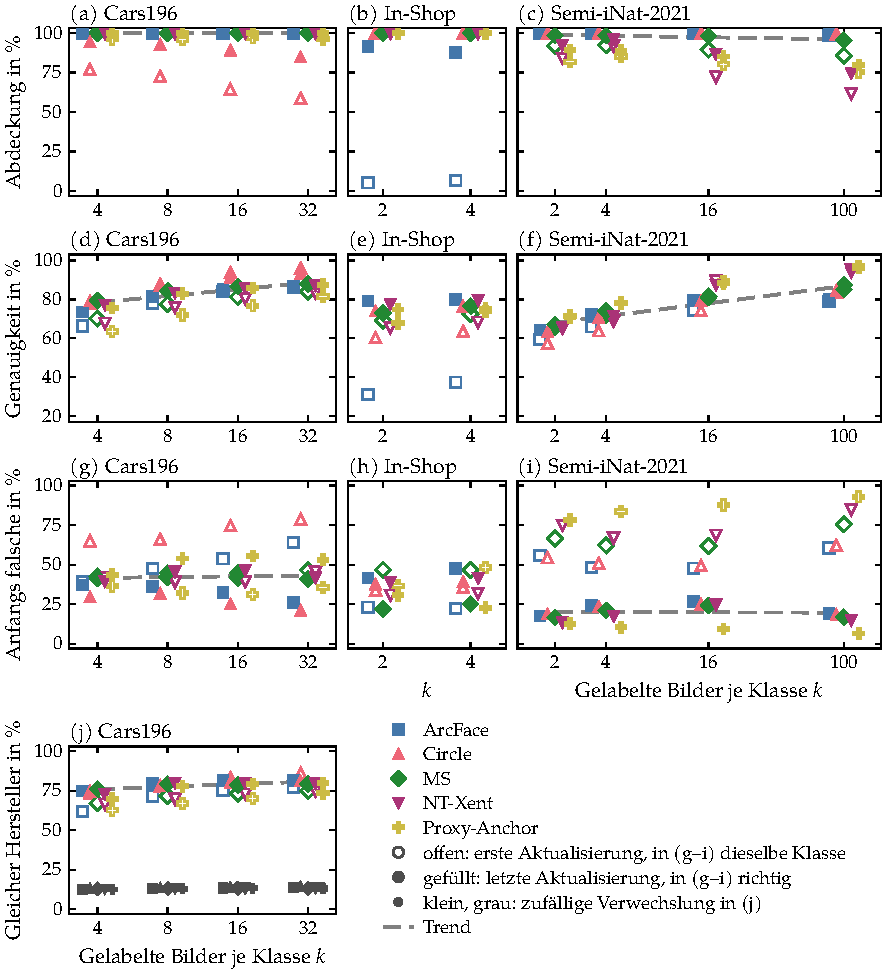
\includegraphics{neu/lp_pseudolabels}
  \caption[Pseudo-Labels von \acs{LP} über die Budgets]{Pseudo-Labels von \acs{LP} in den Geometrieläufen über das Label-Budget $k$, alle fünf Verlustfunktionen, Seed 2, Mittel über die vier Folds. (a--c) Abdeckung und (d--f) Genauigkeit der übernommenen Pseudo-Labels, offen bei der ersten, gefüllt bei der letzten Aktualisierung eines Folds. (g--i) Anteil der anfangs falschen Pseudo-Labels, die bei der letzten Aktualisierung richtig sind (gefüllt) oder noch dieselbe Klasse nennen (offen). (j) Anteil der falschen Pseudo-Labels, die ein Modell desselben Herstellers nennen, offen bei der ersten, gefüllt bei der letzten Aktualisierung, klein und grau bei zufälliger Verwechslung. Grau gestrichelt: Trend über die Verlustfunktionen (lineare Anpassung an den Median der gefüllten Punkte je Budget, auf In-Shop mit zwei Budgets ohne Trend).}
  \label{fig:e:lppseudolabels}
\end{figure}

\begingroup\small\setstretch{1}\setlength{\tabcolsep}{4pt}
\begin{longtable}{@{}>{\raggedright\arraybackslash\hangindent=2em\hangafter=1}p{5.1cm} *{5}{S[table-format=2.2]}@{}}
\caption[Alle Varianten der Phase 2 auf Cars196]{Alle Varianten der Phase 2 auf Cars196 ($k=16$, Seed 2): Test-MAP@R (Mean) in \%. Bezeichnungen wie in Tabelle \ref{tab:phase2:eingriffe} und Abschnitt \ref{sec:m:phase2}, Rauschschwelle $2\sqrt{2}\,\sigma$ in Prozentpunkten (Abschnitt \ref{sec:m:phase2}). Bei \acs{LRML} sind \enquote{ohne Warm-up} und \enquote{Warm-up $= 0$} dieselbe Einstellung. --: Lauf nicht vorhanden.}\label{tab:anhang:phase2}\\
\toprule
Variante & {ArcFace} & {Circle} & {\acs{MS}} & {NT-Xent} & {Proxy-Anchor} \\
\midrule
\endfirsthead
\multicolumn{6}{@{}l}{\small Tabelle \thetable{} (Fortsetzung)}\\
\toprule
Variante & {ArcFace} & {Circle} & {\acs{MS}} & {NT-Xent} & {Proxy-Anchor} \\
\midrule
\endhead
\bottomrule
\endlastfoot
\UEBL & 40.33 & 39.15 & 40.76 & 39.21 & 39.22 \\
\addlinespace
\multicolumn{6}{@{}l}{\textit{LP}} \\*
\quad Rauschschwelle & 0.8 & 0.5 & 0.6 & 0.6 & 0.3 \\
\quad reguläre Konfiguration & 41.95 & 42.28 & 43.30 & 41.37 & 42.60 \\
\quad Wiederholung mit Diagnose & 41.95 & 42.33 & 43.30 & 41.37 & 42.60 \\
\quad SSL-Mechanismus abgeschaltet & 37.45 & 39.04 & 40.56 & 39.19 & 39.94 \\
\quad Hyperparameter der \UEBL & 41.45 & 41.83 & 43.77 & 41.52 & 40.24 \\
\quad ohne Warm-up & 40.96 & 42.40 & 42.88 & 41.38 & 42.60 \\
\quad Pseudo-Labels eingefroren & 41.60 & 41.35 & 42.63 & 41.15 & 41.15 \\
\quad Graph umverdrahtet & 27.72 & 33.71 & 31.02 & 35.08 & 32.62 \\
\quad Oracle-Kanten entfernt & 41.70 & 43.14 & 43.85 & 42.53 & 43.61 \\
\quad zufällige Kanten entfernt & 41.81 & 42.48 & 42.92 & 41.56 & 42.66 \\
\quad Oracle-Labels, 0\,\% Rauschen & 42.09 & 42.91 & 44.17 & 42.42 & 43.55 \\
\quad Oracle-Labels, 10\,\% Rauschen & 42.53 & 37.83 & 41.89 & 42.29 & 41.18 \\
\quad Oracle-Labels, 20\,\% Rauschen & 42.07 & 37.03 & 39.20 & 41.33 & 39.10 \\
\quad Oracle-Labels, 40\,\% Rauschen & 40.21 & 36.18 & 33.74 & 39.06 & 36.21 \\
\quad Oracle-Labels, 60\,\% Rauschen & 38.71 & 35.51 & 31.89 & 36.11 & 33.36 \\
\quad Nachbarzahl $= 2$ & 41.32 & 42.22 & 42.92 & 41.52 & 42.63 \\
\quad Nachbarzahl $= 25$ & 41.62 & 42.34 & 42.69 & 41.26 & 42.66 \\
\quad Nachbarzahl $= 50$ & 41.29 & 42.30 & 42.25 & 41.27 & 42.68 \\
\quad Nachbarzahl $= 75$ & 41.65 & 42.09 & 42.21 & 41.03 & 42.67 \\
\quad Nachbarzahl $= 100$ & 41.61 & 42.10 & 41.68 & 40.71 & 42.55 \\
\quad Nachbarzahl $= 500$ & 41.59 & 39.96 & 38.90 & 40.66 & 37.14 \\
\quad Konfidenzschwelle $= 0{,}1$ & 41.95 & 42.30 & 43.13 & 41.37 & 42.57 \\
\quad Konfidenzschwelle $= 0{,}3$ & 41.95 & 42.30 & 43.13 & 41.37 & 42.57 \\
\quad Konfidenzschwelle $= 0{,}5$ & 41.70 & 42.29 & 43.06 & 41.59 & 42.46 \\
\quad Konfidenzschwelle $= 0{,}7$ & 41.52 & 42.45 & 43.01 & 41.73 & 42.50 \\
\quad Konfidenzschwelle $= 0{,}9$ & 39.23 & 41.67 & 40.89 & 41.14 & 42.68 \\
\quad Warm-up $= 30$ & 40.46 & 42.45 & 41.36 & 41.60 & 42.69 \\
\addlinespace
\multicolumn{6}{@{}l}{\textit{\acs{LRML}}} \\*
\quad Rauschschwelle & 0.5 & 0.7 & 1.1 & 0.7 & 0.5 \\
\quad reguläre Konfiguration & 40.91 & 40.89 & 40.37 & 39.85 & 41.72 \\
\quad SSL-Mechanismus abgeschaltet & 35.56 & 38.80 & 35.96 & 36.72 & 38.64 \\
\quad ohne ungelabelte Bilder & 37.79 & 40.49 & 38.48 & 39.19 & 40.58 \\
\quad Hyperparameter der \UEBL & 36.78 & 40.92 & 40.44 & 36.70 & 37.91 \\
\quad ohne Warm-up & 31.29 & 40.22 & 38.20 & 33.42 & 39.67 \\
\quad Graph eingefroren & 40.40 & 40.72 & 39.75 & 39.98 & 41.62 \\
\quad Graph umverdrahtet & 35.77 & 38.68 & 34.77 & 37.10 & 38.51 \\
\quad Oracle-Kanten entfernt & 41.30 & 41.36 & 41.13 & 40.46 & 42.45 \\
\quad zufällige Kanten entfernt & 41.08 & 40.94 & 40.10 & 40.14 & 41.67 \\
\quad Nachbarzahl $= 2$ & 39.60 & 38.98 & 37.46 & 39.46 & 40.57 \\
\quad Nachbarzahl $= 25$ & 41.05 & 40.38 & 39.99 & 39.69 & 41.58 \\
\quad Nachbarzahl $= 50$ & 41.01 & 40.60 & 40.35 & 39.89 & 41.61 \\
\quad Nachbarzahl $= 75$ & 40.66 & 41.03 & 40.16 & 40.24 & 41.63 \\
\quad Nachbarzahl $= 100$ & 40.03 & 41.10 & 39.67 & 40.07 & 41.21 \\
\quad Nachbarzahl $= 500$ & 37.32 & 40.43 & 35.45 & 39.19 & 40.13 \\
\quad $\eta$ $= 0{,}1$ & 36.16 & 39.25 & 36.32 & 36.96 & 39.02 \\
\quad $\eta$ $= 0{,}2$ & 36.99 & 39.58 & 36.90 & 37.27 & 39.41 \\
\quad $\eta$ $= 0{,}35$ & 38.25 & 40.07 & 37.43 & 37.69 & 39.98 \\
\quad $\eta$ $= 0{,}5$ & 39.73 & 40.54 & 38.23 & 38.10 & 40.48 \\
\quad $\eta$ $= 0{,}75$ & 41.06 & 41.10 & 39.70 & 38.20 & 41.54 \\
\quad $\eta$ $= 1{,}0$ & 41.23 & 41.33 & 40.59 & 39.76 & 41.82 \\
\quad $\eta$ $= 1{,}5$ & 40.44 & 40.55 & 41.30 & 40.64 & 41.68 \\
\quad $\eta$ $= 3{,}0$ & 38.30 & 39.07 & 39.68 & 38.95 & 40.08 \\
\quad Warm-up $= 0$ & 31.29 & 40.22 & 38.20 & 33.42 & 39.67 \\
\quad Warm-up $= 30$ & 40.91 & 40.93 & 40.37 & 37.03 & 41.72 \\
\addlinespace
\multicolumn{6}{@{}l}{\textit{Hoffer}} \\*
\quad Rauschschwelle & 0.3 & 0.4 & 0.5 & 0.7 & 0.5 \\
\quad reguläre Konfiguration & 40.52 & 40.62 & 39.47 & 40.31 & 40.65 \\
\quad SSL-Mechanismus abgeschaltet & 39.20 & 38.89 & 38.56 & 38.11 & 39.56 \\
\quad ohne ungelabelte Bilder & 38.26 & 39.30 & 38.46 & 38.51 & 39.39 \\
\quad Hyperparameter der \UEBL & 40.58 & 39.37 & 39.25 & 39.63 & 39.02 \\
\quad ohne Warm-up & 40.21 & 39.63 & 38.88 & 40.15 & 40.64 \\
\quad $\eta$ $= 0{,}1$ & 40.02 & 39.39 & 38.85 & 38.43 & 39.80 \\
\quad $\eta$ $= 0{,}2$ & 40.43 & 39.77 & 39.10 & 39.48 & 39.98 \\
\quad $\eta$ $= 0{,}35$ & 40.64 & 40.23 & 39.34 & 39.90 & 40.29 \\
\quad $\eta$ $= 0{,}5$ & 40.68 & 40.50 & 39.43 & 40.08 & 40.49 \\
\quad $\eta$ $= 0{,}75$ & 40.30 & 40.64 & 39.54 & 40.16 & 40.85 \\
\quad $\eta$ $= 1{,}0$ & 39.73 & 40.52 & 39.60 & 40.45 & 40.93 \\
\quad $\eta$ $= 1{,}5$ & 38.90 & 40.33 & 39.46 & 40.26 & 41.04 \\
\quad $\eta$ $= 3{,}0$ & 39.14 & 40.28 & 39.39 & 40.19 & 39.87 \\
\quad Distanzskala $\gamma_{\mathrm{H}}$ $= 1$ & 33.78 & 35.48 & 38.00 & 33.32 & 37.05 \\
\quad Distanzskala $\gamma_{\mathrm{H}}$ $= 2$ & 35.21 & 39.65 & 38.45 & 36.40 & 37.17 \\
\quad Distanzskala $\gamma_{\mathrm{H}}$ $= 4$ & 38.10 & 40.53 & 38.76 & 39.22 & 40.92 \\
\quad Distanzskala $\gamma_{\mathrm{H}}$ $= 16$ & 40.29 & 39.54 & 39.64 & 38.72 & 40.40 \\
\quad Distanzskala $\gamma_{\mathrm{H}}$ $= 32$ & 39.88 & 39.02 & 39.22 & 37.95 & 40.06 \\
\quad Distanzskala $\gamma_{\mathrm{H}}$ $= 64$ & 39.57 & 38.90 & 38.90 & 37.59 & 39.89 \\
\quad Distanzskala $\gamma_{\mathrm{H}}$ $= 128$ & 39.47 & 38.80 & 38.48 & 37.61 & 39.69 \\
\quad Distanzskala $\gamma_{\mathrm{H}}$ $= 256$ & 39.52 & 38.69 & 38.50 & 37.55 & 39.65 \\
\quad Distanzskala $\gamma_{\mathrm{H}}$ $= 512$ & 39.47 & 38.81 & 38.41 & 37.37 & 39.77 \\
\addlinespace
\multicolumn{6}{@{}l}{\textit{SLADE}} \\*
\quad Rauschschwelle & 1.0 & 0.6 & 1.0 & 0.3 & 0.6 \\
\quad reguläre Konfiguration & 40.20 & 41.60 & 41.68 & 40.61 & 40.38 \\
\quad SSL-Mechanismus abgeschaltet & 39.50 & 38.55 & 40.16 & 38.31 & 38.86 \\
\quad ohne ungelabelte Bilder & 40.04 & 38.12 & 40.84 & 38.79 & 39.52 \\
\quad Hyperparameter der \UEBL & 35.65 & 41.07 & 38.87 & 35.33 & 38.24 \\
\quad ohne Warm-up & 38.97 & 39.53 & 41.23 & 39.16 & 40.38 \\
\end{longtable}\endgroup

\begingroup\small\setstretch{1}\setlength{\tabcolsep}{4pt}
\begin{longtable}{@{}>{\raggedright\arraybackslash\hangindent=2em\hangafter=1}p{5.1cm} *{5}{S[table-format=2.2]}@{}}
\caption[Alle Varianten der Phase~2 auf In-Shop]{Alle Varianten der Phase~2 auf In-Shop ($k=2$, Seed~2), aufgebaut wie Tabelle~\ref{tab:anhang:phase2}. Fehlende SLADE-Werte: nicht untersucht, Sweeps in Tabelle~\ref{tab:anhang:phase2:slade}. --: Lauf nicht vorhanden.}\label{tab:anhang:phase2:inshop}\\
\toprule
Variante & {ArcFace} & {Circle} & {\acs{MS}} & {NT-Xent} & {Proxy-Anchor} \\
\midrule
\endfirsthead
\multicolumn{6}{@{}l}{\small Tabelle~\thetable{} (Fortsetzung)}\\
\toprule
Variante & {ArcFace} & {Circle} & {\acs{MS}} & {NT-Xent} & {Proxy-Anchor} \\
\midrule
\endhead
\bottomrule
\endlastfoot
\UEBL & 54.80 & 54.70 & 56.09 & 54.60 & 53.81 \\
\addlinespace
\multicolumn{6}{@{}l}{\textit{LP}} \\*
\quad Rauschschwelle & 0.1 & 0.3 & 0.2 & 0.4 & 0.4 \\
\quad reguläre Konfiguration & 58.91 & 57.76 & 58.81 & 57.95 & 56.30 \\
\quad Wiederholung mit Diagnose & 58.91 & 57.77 & 58.81 & 57.95 & 56.30 \\
\quad SSL-Term abgeschaltet & 48.12 & 54.64 & 55.77 & 53.73 & 52.87 \\
\quad ohne ungelabelte Bilder & 52.22 & 54.54 & 55.80 & 53.70 & 52.92 \\
\quad Hyperparameter der \UEBL & 58.21 & 56.72 & 58.98 & 57.28 & 53.71 \\
\quad ohne Warm-up & 58.79 & 57.64 & 59.00 & 57.82 & 55.87 \\
\quad Pseudo-Labels eingefroren & 47.43 & 55.21 & 58.16 & 55.80 & 55.00 \\
\quad Graph umverdrahtet & 45.51 & 47.59 & 49.35 & 46.47 & 47.36 \\
\quad Oracle-Kanten entfernt & 50.69 & 59.92 & 60.17 & 59.62 & 58.32 \\
\quad zufällige Kanten entfernt & 36.27 & 53.67 & 58.98 & 58.04 & 56.20 \\
\quad Oracle-Labels, 0\,\% Rauschen & 60.81 & 59.73 & 60.40 & 59.61 & 58.98 \\
\quad Oracle-Labels, 10\,\% Rauschen & 59.42 & 55.84 & 57.31 & 55.07 & 56.90 \\
\quad Oracle-Labels, 20\,\% Rauschen & 57.79 & 53.68 & 54.08 & 52.59 & 55.11 \\
\quad Oracle-Labels, 40\,\% Rauschen & 53.56 & 50.31 & 50.98 & 49.34 & 51.79 \\
\quad Oracle-Labels, 60\,\% Rauschen & 48.42 & 47.87 & 50.07 & 47.06 & 49.07 \\
\quad Nachbarzahl $= 2$ & 42.74 & 58.49 & 59.23 & 57.95 & 56.30 \\
\quad Nachbarzahl $= 25$ & 37.77 & 57.71 & 58.61 & 57.54 & 54.50 \\
\quad Nachbarzahl $= 50$ & 37.04 & 57.79 & 58.60 & 55.87 & 54.45 \\
\quad Nachbarzahl $= 75$ & 58.76 & 57.70 & 58.64 & 54.21 & 54.34 \\
\quad Nachbarzahl $= 100$ & 58.93 & 57.78 & 58.79 & 53.49 & 54.45 \\
\quad Nachbarzahl $= 500$ & 57.70 & 57.79 & 58.59 & 52.96 & 54.67 \\
\quad Konfidenzschwelle $= 0{,}1$ & 37.15 & 57.77 & 58.81 & 57.95 & 56.30 \\
\quad Konfidenzschwelle $= 0{,}3$ & 37.15 & 57.77 & 58.81 & 57.95 & 56.30 \\
\quad Konfidenzschwelle $= 0{,}5$ & 37.19 & 57.71 & 58.81 & 57.95 & 56.30 \\
\quad Konfidenzschwelle $= 0{,}7$ & 36.41 & 54.81 & 58.85 & 57.77 & 56.23 \\
\quad Konfidenzschwelle $= 0{,}9$ & 29.48 & 54.14 & 58.80 & 58.18 & 56.82 \\
\quad Warm-up $= 30$ & 58.89 & 57.85 & 58.82 & 57.94 & 56.30 \\
\addlinespace
\multicolumn{6}{@{}l}{\textit{\acs{LRML}}} \\*
\quad Rauschschwelle & 1.3 & 0.3 & 0.7 & 0.4 & 0.7 \\
\quad reguläre Konfiguration & 58.03 & 57.58 & 56.57 & 55.72 & 53.68 \\
\quad SSL-Term abgeschaltet & 47.00 & 52.95 & 54.11 & 53.17 & 50.97 \\
\quad ohne ungelabelte Bilder & 54.74 & 53.46 & 53.80 & 53.23 & 51.42 \\
\quad Hyperparameter der \UEBL & 52.42 & 56.00 & 57.17 & 54.68 & 54.07 \\
\quad ohne Warm-up & 49.60 & 57.30 & 56.23 & 55.66 & 54.36 \\
\quad Graph eingefroren & 56.70 & 55.75 & 56.37 & 55.40 & 51.36 \\
\quad Graph umverdrahtet & 46.63 & 45.94 & 52.17 & 50.82 & 51.12 \\
\quad Oracle-Kanten entfernt & 59.22 & 58.94 & 57.47 & 56.97 & 54.39 \\
\quad zufällige Kanten entfernt & 57.95 & 57.47 & 56.66 & 55.80 & 53.83 \\
\quad Nachbarzahl $= 2$ & 57.70 & 57.48 & 56.57 & 55.93 & 53.90 \\
\quad Nachbarzahl $= 25$ & 53.39 & 52.91 & 53.86 & 53.49 & 51.93 \\
\quad Nachbarzahl $= 50$ & 52.00 & 51.05 & 53.64 & 53.18 & 51.47 \\
\quad Nachbarzahl $= 75$ & 51.36 & 50.86 & 53.73 & 53.11 & 51.58 \\
\quad Nachbarzahl $= 100$ & 50.84 & 50.94 & 53.73 & 53.17 & 51.48 \\
\quad Nachbarzahl $= 500$ & 48.84 & 49.08 & 53.69 & 53.23 & 51.50 \\
\quad $\eta$ $= 0{,}1$ & 48.67 & 53.99 & 54.59 & 53.98 & 51.58 \\
\quad $\eta$ $= 0{,}2$ & 50.77 & 55.18 & 55.19 & 54.66 & 52.20 \\
\quad $\eta$ $= 0{,}35$ & 54.37 & 56.68 & 56.06 & 55.46 & 52.96 \\
\quad $\eta$ $= 0{,}5$ & 57.36 & 57.75 & 56.63 & 55.85 & 53.68 \\
\quad $\eta$ $= 0{,}75$ & 56.77 & 47.73 & 53.44 & 55.55 & 54.34 \\
\quad $\eta$ $= 1{,}0$ & 50.22 & 46.62 & 51.29 & 52.25 & 54.66 \\
\quad $\eta$ $= 1{,}5$ & 46.35 & 44.87 & 50.17 & 50.02 & 52.10 \\
\quad $\eta$ $= 3{,}0$ & 43.00 & 44.91 & 48.59 & 45.11 & 33.63 \\
\quad Warm-up $= 0$ & 49.60 & 57.30 & 56.23 & 55.66 & 54.36 \\
\quad Warm-up $= 30$ & 58.03 & 57.72 & 56.71 & 55.87 & 53.85 \\
\addlinespace
\multicolumn{6}{@{}l}{\textit{Hoffer}} \\*
\quad Rauschschwelle & 0.2 & 0.2 & 0.2 & 0.2 & 0.3 \\
\quad reguläre Konfiguration & 57.75 & 58.05 & 57.90 & 58.21 & 57.56 \\
\quad SSL-Term abgeschaltet & 52.70 & 54.35 & 53.05 & 51.96 & 51.88 \\
\quad ohne ungelabelte Bilder & 53.62 & 54.49 & 53.89 & 54.70 & 53.60 \\
\quad Hyperparameter der \UEBL & 57.19 & 57.50 & 56.97 & 57.11 & 56.60 \\
\quad ohne Warm-up & 57.24 & 57.98 & 57.68 & 58.05 & 57.56 \\
\quad $\eta$ $= 0{,}1$ & 54.06 & 54.82 & 54.69 & 54.17 & 53.25 \\
\quad $\eta$ $= 0{,}2$ & 55.03 & 55.37 & 55.78 & 55.58 & 54.32 \\
\quad $\eta$ $= 0{,}35$ & 56.10 & 55.97 & 56.62 & 56.91 & 55.51 \\
\quad $\eta$ $= 0{,}5$ & 56.67 & 56.53 & 57.12 & 57.59 & 56.25 \\
\quad $\eta$ $= 0{,}75$ & 57.34 & 57.29 & 57.54 & 58.12 & 56.92 \\
\quad $\eta$ $= 1{,}0$ & 57.67 & 57.68 & 57.73 & 58.30 & 57.36 \\
\quad $\eta$ $= 1{,}5$ & 57.75 & 57.98 & 58.02 & 58.32 & 57.60 \\
\quad $\eta$ $= 3{,}0$ & 56.95 & 57.67 & 58.13 & 58.01 & 56.93 \\
\quad Distanzskala $\gamma_{\mathrm{H}}$ $= 1$ & 33.53 & 40.94 & 34.15 & 38.65 & 13.21 \\
\quad Distanzskala $\gamma_{\mathrm{H}}$ $= 2$ & 30.34 & 35.91 & 34.47 & 41.68 & 6.15 \\
\quad Distanzskala $\gamma_{\mathrm{H}}$ $= 4$ & 38.94 & 43.85 & 44.29 & 44.81 & 16.37 \\
\quad Distanzskala $\gamma_{\mathrm{H}}$ $= 16$ & 56.95 & 56.43 & 57.06 & 57.41 & 56.83 \\
\quad Distanzskala $\gamma_{\mathrm{H}}$ $= 32$ & 55.10 & 55.12 & 54.80 & 55.10 & 54.97 \\
\quad Distanzskala $\gamma_{\mathrm{H}}$ $= 64$ & 53.53 & 54.46 & 53.23 & 53.02 & 52.90 \\
\quad Distanzskala $\gamma_{\mathrm{H}}$ $= 128$ & 52.68 & 54.17 & 52.86 & 52.20 & 51.29 \\
\quad Distanzskala $\gamma_{\mathrm{H}}$ $= 256$ & 52.26 & 54.10 & 52.72 & 52.03 & 50.61 \\
\quad Distanzskala $\gamma_{\mathrm{H}}$ $= 512$ & 51.96 & 54.05 & 52.67 & 51.93 & 50.24 \\
\addlinespace
\multicolumn{6}{@{}l}{\textit{SLADE}} \\*
\quad Rauschschwelle & 1.4 & 0.4 & 0.4 & 0.5 & 0.9 \\
\quad reguläre Konfiguration & 53.69 & 54.77 & 54.49 & 54.14 & 53.71 \\
\quad SSL-Term abgeschaltet & 52.66 & 54.71 & 52.65 & 54.16 & 43.10 \\
\quad ohne ungelabelte Bilder & 54.03 & 54.49 & 53.98 & 54.22 & 53.71 \\
\quad Hyperparameter der \UEBL & 46.61 & 53.39 & 51.05 & 53.86 & 52.14 \\
\quad ohne Warm-up & 53.69 & 54.56 & 54.35 & 54.27 & 53.65 \\
\end{longtable}\endgroup

\begingroup\small\setstretch{1}\setlength{\tabcolsep}{4pt}
\begin{longtable}{@{}>{\raggedright\arraybackslash\hangindent=2em\hangafter=1}p{5.1cm} *{5}{S[table-format=2.2]}@{}}
\caption[Alle Varianten der Phase~2 auf Cars196 als Ensemble]{Alle Varianten der Phase~2 auf Cars196 wie in Tabelle~\ref{tab:anhang:phase2}, aber für das Ensemble (Test-MAP@R Concat in \%). Rauschschwelle aus der Seed-Standardabweichung der Concat-MAP@R in Phase~1 (Abschnitt~\ref{sec:m:phase2}).}\label{tab:anhang:phase2:concat}\\
\toprule
Variante & {ArcFace} & {Circle} & {\acs{MS}} & {NT-Xent} & {Proxy-Anchor} \\
\midrule
\endfirsthead
\multicolumn{6}{@{}l}{\small Tabelle~\thetable{} (Fortsetzung)}\\
\toprule
Variante & {ArcFace} & {Circle} & {\acs{MS}} & {NT-Xent} & {Proxy-Anchor} \\
\midrule
\endhead
\bottomrule
\endlastfoot
\UEBL & 43.41 & 42.66 & 44.20 & 42.53 & 42.84 \\
Rauschschwelle \UEBL & 0.7 & 0.5 & 0.6 & 0.7 & 0.9 \\
\addlinespace
\multicolumn{6}{@{}l}{\textit{LP}} \\*
\quad Rauschschwelle & 0.5 & 0.6 & 0.3 & 0.3 & 0.3 \\
\quad reguläre Konfiguration & 44.59 & 44.65 & 46.23 & 44.29 & 45.06 \\
\quad Wiederholung mit Diagnose & 44.59 & 44.72 & 46.23 & 44.29 & 45.06 \\
\quad SSL-Term abgeschaltet & 41.61 & 41.99 & 43.92 & 42.50 & 42.87 \\
\quad ohne ungelabelte Bilder & 41.45 & 42.02 & 44.18 & 42.55 & 42.96 \\
\quad Hyperparameter der \UEBL & 43.96 & 44.88 & 45.92 & 44.22 & 44.16 \\
\quad ohne Warm-up & 43.78 & 44.92 & 46.08 & 44.21 & 45.05 \\
\quad Pseudo-Labels eingefroren & 44.36 & 44.14 & 45.85 & 43.95 & 43.82 \\
\quad Graph umverdrahtet & 30.98 & 35.39 & 32.09 & 36.23 & 32.93 \\
\quad Oracle-Kanten entfernt & 44.49 & 45.13 & 46.67 & 44.82 & 45.59 \\
\quad zufällige Kanten entfernt & 44.49 & 44.89 & 45.94 & 44.35 & 45.17 \\
\quad Oracle-Labels, 0\,\% Rauschen & 44.72 & 45.18 & 46.78 & 44.82 & 45.56 \\
\quad Oracle-Labels, 10\,\% Rauschen & 45.12 & 38.96 & 45.04 & 44.64 & 44.23 \\
\quad Oracle-Labels, 20\,\% Rauschen & 44.93 & 38.12 & 42.33 & 44.09 & 42.23 \\
\quad Oracle-Labels, 40\,\% Rauschen & 44.12 & 37.21 & 36.43 & 41.57 & 38.64 \\
\quad Oracle-Labels, 60\,\% Rauschen & 42.67 & 36.54 & 33.00 & 38.01 & 34.75 \\
\quad Nachbarzahl $= 2$ & 44.28 & 44.72 & 46.14 & 44.40 & 45.16 \\
\quad Nachbarzahl $= 25$ & 44.47 & 44.85 & 45.82 & 44.20 & 45.15 \\
\quad Nachbarzahl $= 50$ & 44.12 & 44.88 & 45.53 & 44.08 & 45.05 \\
\quad Nachbarzahl $= 75$ & 44.35 & 44.92 & 45.37 & 43.84 & 45.00 \\
\quad Nachbarzahl $= 100$ & 44.23 & 44.88 & 44.96 & 43.61 & 44.93 \\
\quad Nachbarzahl $= 500$ & 44.34 & 43.10 & 40.36 & 43.48 & 40.09 \\
\quad Konfidenzschwelle $= 0{,}1$ & 44.59 & 44.80 & 46.16 & 44.29 & 45.07 \\
\quad Konfidenzschwelle $= 0{,}3$ & 44.59 & 44.80 & 46.16 & 44.29 & 45.07 \\
\quad Konfidenzschwelle $= 0{,}5$ & 44.32 & 44.74 & 46.08 & 44.30 & 45.06 \\
\quad Konfidenzschwelle $= 0{,}7$ & 44.41 & 44.77 & 46.09 & 44.42 & 45.10 \\
\quad Konfidenzschwelle $= 0{,}9$ & 43.19 & 44.59 & 45.14 & 44.34 & 45.10 \\
\quad Warm-up $= 30$ & 43.81 & 44.94 & 45.52 & 44.42 & 45.10 \\
\addlinespace
\multicolumn{6}{@{}l}{\textit{\acs{LRML}}} \\*
\quad Rauschschwelle & 0.7 & 0.7 & 0.6 & 0.8 & 0.3 \\
\quad reguläre Konfiguration & 44.39 & 44.48 & 45.20 & 43.97 & 45.22 \\
\quad SSL-Term abgeschaltet & 39.89 & 41.64 & 40.72 & 41.81 & 41.28 \\
\quad ohne ungelabelte Bilder & 41.38 & 43.38 & 43.39 & 43.57 & 42.71 \\
\quad Hyperparameter der \UEBL & 37.44 & 43.44 & 41.63 & 37.31 & 42.90 \\
\quad ohne Warm-up & 37.50 & 44.24 & 43.36 & 39.67 & 44.13 \\
\quad Graph eingefroren & 44.40 & 44.46 & 45.21 & 44.28 & 45.10 \\
\quad Graph umverdrahtet & 40.11 & 40.80 & 39.46 & 41.92 & 40.37 \\
\quad Oracle-Kanten entfernt & 44.83 & 45.03 & 45.67 & 44.31 & 45.55 \\
\quad zufällige Kanten entfernt & 44.47 & 44.46 & 45.12 & 44.05 & 45.20 \\
\quad Nachbarzahl $= 2$ & 42.64 & 42.54 & 41.44 & 43.45 & 44.27 \\
\quad Nachbarzahl $= 25$ & 44.30 & 44.09 & 44.63 & 43.77 & 45.14 \\
\quad Nachbarzahl $= 50$ & 44.45 & 44.38 & 45.16 & 43.99 & 45.22 \\
\quad Nachbarzahl $= 75$ & 44.25 & 44.43 & 45.13 & 44.20 & 45.19 \\
\quad Nachbarzahl $= 100$ & 43.71 & 44.27 & 44.99 & 44.10 & 44.74 \\
\quad Nachbarzahl $= 500$ & 41.44 & 43.01 & 41.74 & 43.85 & 42.46 \\
\quad $\eta$ $= 0{,}1$ & 40.59 & 42.17 & 41.49 & 42.14 & 41.72 \\
\quad $\eta$ $= 0{,}2$ & 41.48 & 43.04 & 42.98 & 42.37 & 42.08 \\
\quad $\eta$ $= 0{,}35$ & 42.87 & 43.97 & 43.62 & 42.75 & 42.83 \\
\quad $\eta$ $= 0{,}5$ & 43.93 & 44.39 & 44.34 & 43.14 & 43.59 \\
\quad $\eta$ $= 0{,}75$ & 44.49 & 44.35 & 45.13 & 43.57 & 44.70 \\
\quad $\eta$ $= 1{,}0$ & 43.90 & 43.30 & 45.37 & 43.88 & 45.27 \\
\quad $\eta$ $= 1{,}5$ & 42.98 & 42.37 & 44.99 & 43.92 & 43.28 \\
\quad $\eta$ $= 3{,}0$ & 40.58 & 40.62 & 43.06 & 41.50 & 41.30 \\
\quad Warm-up $= 0$ & 37.50 & 44.24 & 43.36 & 39.67 & 44.13 \\
\quad Warm-up $= 30$ & 44.39 & 44.63 & 45.20 & 42.89 & 45.22 \\
\addlinespace
\multicolumn{6}{@{}l}{\textit{Hoffer}} \\*
\quad Rauschschwelle & 0.6 & 0.5 & 0.6 & 0.7 & 0.6 \\
\quad reguläre Konfiguration & 44.13 & 44.34 & 43.46 & 44.22 & 44.03 \\
\quad SSL-Term abgeschaltet & 42.49 & 41.82 & 42.08 & 40.16 & 42.75 \\
\quad ohne ungelabelte Bilder & 41.73 & 42.74 & 42.31 & 42.25 & 42.58 \\
\quad Hyperparameter der \UEBL & 44.16 & 43.36 & 43.43 & 43.72 & 43.41 \\
\quad ohne Warm-up & 44.02 & 43.88 & 43.10 & 44.06 & 43.89 \\
\quad $\eta$ $= 0{,}1$ & 43.40 & 42.67 & 42.79 & 41.71 & 43.03 \\
\quad $\eta$ $= 0{,}2$ & 43.82 & 43.51 & 43.13 & 43.06 & 43.33 \\
\quad $\eta$ $= 0{,}35$ & 44.12 & 44.10 & 43.41 & 43.65 & 43.62 \\
\quad $\eta$ $= 0{,}5$ & 44.18 & 44.27 & 43.50 & 43.89 & 43.89 \\
\quad $\eta$ $= 0{,}75$ & 44.07 & 44.36 & 43.55 & 44.12 & 44.15 \\
\quad $\eta$ $= 1{,}0$ & 43.78 & 44.28 & 43.51 & 44.21 & 44.26 \\
\quad $\eta$ $= 1{,}5$ & 43.24 & 44.14 & 43.44 & 44.22 & 44.21 \\
\quad $\eta$ $= 3{,}0$ & 42.90 & 43.93 & 43.57 & 44.20 & 43.74 \\
\quad Distanzskala $\gamma_{\mathrm{H}}$ $= 1$ & 34.59 & 37.93 & 39.44 & 34.79 & 40.16 \\
\quad Distanzskala $\gamma_{\mathrm{H}}$ $= 2$ & 35.94 & 41.82 & 39.98 & 37.96 & 39.48 \\
\quad Distanzskala $\gamma_{\mathrm{H}}$ $= 4$ & 42.42 & 44.39 & 43.07 & 43.49 & 43.96 \\
\quad Distanzskala $\gamma_{\mathrm{H}}$ $= 16$ & 43.68 & 42.74 & 43.03 & 41.83 & 43.74 \\
\quad Distanzskala $\gamma_{\mathrm{H}}$ $= 32$ & 43.34 & 42.53 & 42.72 & 41.00 & 43.32 \\
\quad Distanzskala $\gamma_{\mathrm{H}}$ $= 64$ & 43.00 & 42.19 & 42.25 & 40.61 & 42.98 \\
\quad Distanzskala $\gamma_{\mathrm{H}}$ $= 128$ & 42.79 & 42.09 & 42.17 & 40.75 & 42.89 \\
\quad Distanzskala $\gamma_{\mathrm{H}}$ $= 256$ & 42.68 & 41.90 & 42.08 & 40.20 & 42.83 \\
\quad Distanzskala $\gamma_{\mathrm{H}}$ $= 512$ & 42.63 & 41.76 & 41.96 & 40.19 & 42.83 \\
\addlinespace
\multicolumn{6}{@{}l}{\textit{SLADE}} \\*
\quad Rauschschwelle & 0.7 & 0.7 & 0.7 & 0.7 & 0.6 \\
\quad reguläre Konfiguration & 43.51 & 44.91 & 44.95 & 44.26 & 43.62 \\
\quad SSL-Term abgeschaltet & 42.73 & 41.52 & 43.38 & 41.36 & 41.41 \\
\quad ohne ungelabelte Bilder & 42.34 & 43.03 & 44.42 & 42.58 & 42.62 \\
\quad Hyperparameter der \UEBL & 39.44 & 43.52 & 43.27 & 39.81 & 42.66 \\
\quad ohne Warm-up & 42.77 & 43.36 & 44.37 & 43.59 & 43.62 \\
\end{longtable}\endgroup

\begingroup\small\setstretch{1}\setlength{\tabcolsep}{4pt}
\begin{longtable}{@{}>{\raggedright\arraybackslash\hangindent=2em\hangafter=1}p{5.1cm} *{5}{S[table-format=2.2]}@{}}
\caption[Alle Varianten der Phase~2 auf In-Shop als Ensemble]{Alle Varianten der Phase~2 auf In-Shop wie in Tabelle~\ref{tab:anhang:phase2:inshop}, aber für das Ensemble (Test-MAP@R Concat in \%). Rauschschwelle aus der Seed-Standardabweichung der Concat-MAP@R in Phase~1 (Abschnitt~\ref{sec:m:phase2}).}\label{tab:anhang:phase2:inshop:concat}\\
\toprule
Variante & {ArcFace} & {Circle} & {\acs{MS}} & {NT-Xent} & {Proxy-Anchor} \\
\midrule
\endfirsthead
\multicolumn{6}{@{}l}{\small Tabelle~\thetable{} (Fortsetzung)}\\
\toprule
Variante & {ArcFace} & {Circle} & {\acs{MS}} & {NT-Xent} & {Proxy-Anchor} \\
\midrule
\endhead
\bottomrule
\endlastfoot
\UEBL & 57.45 & 57.61 & 58.84 & 57.29 & 55.97 \\
Rauschschwelle \UEBL & 0.2 & 0.6 & 0.4 & 0.3 & 0.4 \\
\addlinespace
\multicolumn{6}{@{}l}{\textit{LP}} \\*
\quad Rauschschwelle & 0.1 & 0.3 & 0.4 & 0.6 & 0.5 \\
\quad reguläre Konfiguration & 60.62 & 60.06 & 61.08 & 60.23 & 57.22 \\
\quad Wiederholung mit Diagnose & 60.62 & 60.01 & 61.08 & 60.23 & 57.22 \\
\quad SSL-Term abgeschaltet & 50.90 & 57.59 & 59.05 & 56.62 & 54.80 \\
\quad ohne ungelabelte Bilder & 55.76 & 57.49 & 58.80 & 56.50 & 54.91 \\
\quad Hyperparameter der \UEBL & 59.41 & 59.03 & 60.96 & 58.92 & 54.97 \\
\quad ohne Warm-up & 60.53 & 59.90 & 61.35 & 59.93 & 56.88 \\
\quad Pseudo-Labels eingefroren & 52.04 & 57.35 & 60.34 & 57.91 & 56.02 \\
\quad Graph umverdrahtet & 48.44 & 49.10 & 50.74 & 48.68 & 48.21 \\
\quad Oracle-Kanten entfernt & 51.88 & 61.79 & 62.19 & 61.62 & 59.20 \\
\quad zufällige Kanten entfernt & 37.77 & 55.74 & 61.21 & 60.10 & 57.12 \\
\quad Oracle-Labels, 0\,\% Rauschen & 62.04 & 61.36 & 62.55 & 61.35 & 59.73 \\
\quad Oracle-Labels, 10\,\% Rauschen & 61.27 & 58.49 & 60.01 & 57.47 & 58.42 \\
\quad Oracle-Labels, 20\,\% Rauschen & 60.30 & 56.49 & 56.56 & 55.04 & 57.44 \\
\quad Oracle-Labels, 40\,\% Rauschen & 57.20 & 52.96 & 52.25 & 51.53 & 53.93 \\
\quad Oracle-Labels, 60\,\% Rauschen & 53.00 & 50.28 & 51.44 & 49.43 & 50.50 \\
\quad Nachbarzahl $= 2$ & 44.20 & 60.50 & 61.71 & 60.23 & 57.22 \\
\quad Nachbarzahl $= 25$ & 39.21 & 59.90 & 60.81 & 59.72 & 55.64 \\
\quad Nachbarzahl $= 50$ & 38.67 & 59.99 & 60.96 & 58.56 & 55.73 \\
\quad Nachbarzahl $= 75$ & 60.54 & 59.87 & 61.08 & 56.90 & 55.44 \\
\quad Nachbarzahl $= 100$ & 60.56 & 60.08 & 61.25 & 56.65 & 55.60 \\
\quad Nachbarzahl $= 500$ & 59.87 & 60.02 & 60.72 & 56.21 & 55.85 \\
\quad Konfidenzschwelle $= 0{,}1$ & 38.61 & 60.01 & 61.08 & 60.23 & 57.22 \\
\quad Konfidenzschwelle $= 0{,}3$ & 38.61 & 60.01 & 61.08 & 60.23 & 57.22 \\
\quad Konfidenzschwelle $= 0{,}5$ & 38.73 & 59.72 & 61.08 & 60.23 & 57.22 \\
\quad Konfidenzschwelle $= 0{,}7$ & 57.07 & 57.72 & 61.19 & 59.84 & 57.11 \\
\quad Konfidenzschwelle $= 0{,}9$ & 33.60 & 57.37 & 61.11 & 60.34 & 57.67 \\
\quad Warm-up $= 30$ & 60.51 & 60.06 & 61.09 & 60.10 & 57.16 \\
\addlinespace
\multicolumn{6}{@{}l}{\textit{\acs{LRML}}} \\*
\quad Rauschschwelle & 1.3 & 0.3 & 0.7 & 0.7 & 0.5 \\
\quad reguläre Konfiguration & 60.14 & 59.26 & 59.60 & 59.44 & 55.93 \\
\quad SSL-Term abgeschaltet & 49.33 & 55.26 & 57.44 & 56.30 & 53.98 \\
\quad ohne ungelabelte Bilder & 57.53 & 56.25 & 56.75 & 57.04 & 54.16 \\
\quad Hyperparameter der \UEBL & 53.28 & 58.10 & 59.46 & 57.28 & 56.32 \\
\quad ohne Warm-up & 51.14 & 59.40 & 59.63 & 59.46 & 55.97 \\
\quad Graph eingefroren & 59.46 & 57.37 & 59.23 & 58.73 & 53.74 \\
\quad Graph umverdrahtet & 48.82 & 46.56 & 54.85 & 53.23 & 53.98 \\
\quad Oracle-Kanten entfernt & 61.26 & 60.47 & 60.31 & 60.40 & 56.58 \\
\quad zufällige Kanten entfernt & 60.15 & 59.18 & 59.63 & 59.34 & 56.11 \\
\quad Nachbarzahl $= 2$ & 59.38 & 59.05 & 59.60 & 59.36 & 56.01 \\
\quad Nachbarzahl $= 25$ & 56.88 & 56.22 & 57.05 & 57.39 & 54.68 \\
\quad Nachbarzahl $= 50$ & 55.57 & 54.29 & 57.12 & 57.20 & 54.05 \\
\quad Nachbarzahl $= 75$ & 54.95 & 54.13 & 56.95 & 56.98 & 54.28 \\
\quad Nachbarzahl $= 100$ & 54.66 & 53.87 & 56.93 & 57.05 & 54.23 \\
\quad Nachbarzahl $= 500$ & 52.13 & 51.15 & 56.83 & 57.19 & 54.33 \\
\quad $\eta$ $= 0{,}1$ & 51.58 & 56.33 & 57.72 & 57.39 & 54.52 \\
\quad $\eta$ $= 0{,}2$ & 53.91 & 57.64 & 58.48 & 58.36 & 54.89 \\
\quad $\eta$ $= 0{,}35$ & 57.69 & 58.85 & 59.50 & 59.12 & 55.45 \\
\quad $\eta$ $= 0{,}5$ & 60.28 & 59.70 & 59.74 & 59.41 & 55.99 \\
\quad $\eta$ $= 0{,}75$ & 58.80 & 48.40 & 56.37 & 59.19 & 56.16 \\
\quad $\eta$ $= 1{,}0$ & 51.87 & 47.35 & 52.36 & 55.11 & 56.33 \\
\quad $\eta$ $= 1{,}5$ & 47.33 & 45.22 & 51.27 & 51.66 & 53.59 \\
\quad $\eta$ $= 3{,}0$ & 44.33 & 45.30 & 49.62 & 46.51 & 37.03 \\
\quad Warm-up $= 0$ & 51.14 & 59.40 & 59.63 & 59.46 & 55.97 \\
\quad Warm-up $= 30$ & 60.14 & 59.44 & 59.79 & 59.57 & 56.13 \\
\addlinespace
\multicolumn{6}{@{}l}{\textit{Hoffer}} \\*
\quad Rauschschwelle & 0.4 & 0.3 & 0.3 & 0.5 & 0.2 \\
\quad reguläre Konfiguration & 60.35 & 60.37 & 60.66 & 60.78 & 60.00 \\
\quad SSL-Term abgeschaltet & 55.89 & 57.20 & 56.77 & 55.87 & 54.60 \\
\quad ohne ungelabelte Bilder & 56.82 & 57.09 & 57.04 & 57.97 & 57.41 \\
\quad Hyperparameter der \UEBL & 59.66 & 59.65 & 59.50 & 59.23 & 58.37 \\
\quad ohne Warm-up & 60.00 & 60.20 & 60.61 & 60.38 & 60.00 \\
\quad $\eta$ $= 0{,}1$ & 56.95 & 57.81 & 58.52 & 57.72 & 55.85 \\
\quad $\eta$ $= 0{,}2$ & 57.93 & 58.38 & 59.24 & 58.91 & 56.80 \\
\quad $\eta$ $= 0{,}35$ & 58.64 & 58.96 & 59.87 & 59.89 & 57.76 \\
\quad $\eta$ $= 0{,}5$ & 59.57 & 59.38 & 60.14 & 60.25 & 58.51 \\
\quad $\eta$ $= 0{,}75$ & 59.98 & 59.96 & 60.47 & 60.71 & 59.34 \\
\quad $\eta$ $= 1{,}0$ & 60.31 & 60.09 & 60.51 & 60.73 & 59.82 \\
\quad $\eta$ $= 1{,}5$ & 60.34 & 60.13 & 60.61 & 60.50 & 60.09 \\
\quad $\eta$ $= 3{,}0$ & 59.65 & 59.64 & 60.81 & 60.01 & 59.65 \\
\quad Distanzskala $\gamma_{\mathrm{H}}$ $= 1$ & 34.47 & 45.09 & 35.95 & 39.76 & 8.48 \\
\quad Distanzskala $\gamma_{\mathrm{H}}$ $= 2$ & 31.44 & 38.87 & 36.04 & 42.91 & 6.43 \\
\quad Distanzskala $\gamma_{\mathrm{H}}$ $= 4$ & 39.89 & 46.06 & 45.59 & 45.95 & 20.23 \\
\quad Distanzskala $\gamma_{\mathrm{H}}$ $= 16$ & 60.10 & 59.18 & 60.13 & 60.29 & 59.51 \\
\quad Distanzskala $\gamma_{\mathrm{H}}$ $= 32$ & 58.32 & 58.15 & 58.43 & 58.57 & 57.37 \\
\quad Distanzskala $\gamma_{\mathrm{H}}$ $= 64$ & 56.74 & 57.46 & 56.67 & 56.43 & 55.26 \\
\quad Distanzskala $\gamma_{\mathrm{H}}$ $= 128$ & 55.79 & 57.21 & 56.65 & 55.57 & 53.64 \\
\quad Distanzskala $\gamma_{\mathrm{H}}$ $= 256$ & 55.49 & 56.96 & 56.60 & 55.56 & 53.07 \\
\quad Distanzskala $\gamma_{\mathrm{H}}$ $= 512$ & 55.10 & 57.07 & 56.46 & 55.40 & 52.61 \\
\addlinespace
\multicolumn{6}{@{}l}{\textit{SLADE}} \\*
\quad Rauschschwelle & 1.4 & 0.7 & 0.6 & 0.5 & 0.4 \\
\quad reguläre Konfiguration & 56.92 & 56.85 & 57.53 & 56.80 & 57.77 \\
\quad SSL-Term abgeschaltet & 54.98 & 57.29 & 55.49 & 57.18 & 49.90 \\
\quad ohne ungelabelte Bilder & 57.08 & 56.65 & 57.30 & 57.22 & 57.79 \\
\quad Hyperparameter der \UEBL & 49.57 & 55.55 & 52.13 & 55.93 & 54.38 \\
\quad ohne Warm-up & 56.92 & 56.61 & 57.34 & 56.99 & 57.94 \\
\end{longtable}\endgroup

\begin{table}[p]
\centering
\caption[Sweeps von SLADE in Phase 2]{Sweeps einzelner Hyperparameter von SLADE (Phase 2, Seed 2, Cars196 mit $k=16$, In-Shop mit $k=2$): Änderung der Test-MAP@R (Mean) gegenüber der regulären SLADE-Konfiguration in Prozentpunkten. Fett: Betrag über der Rauschschwelle $2\sqrt{2}\,\sigma$, kursiv: in Phase 1 gewählter Wert (Wiederholung der regulären Konfiguration, bei der Teacher-Aktualisierung alle 5 Epochen die reguläre Konfiguration selbst). $^\dagger$: außerhalb der Suchräume der Phase 1 (Clusterverhältnis 0,5 nur auf Cars196). Arc: ArcFace, Cir: Circle, NT: NT-Xent, PA: Proxy-Anchor.}
\label{tab:anhang:phase2:slade}
\small\setlength{\tabcolsep}{3.2pt}
\begin{tabular}{@{}lrrrrrrrrrr@{}}
\toprule
 & \multicolumn{5}{c}{Cars196} & \multicolumn{5}{c}{In-Shop} \\
\cmidrule(lr){2-6}\cmidrule(lr){7-11}
Wert & Arc & Cir & \acs{MS} & NT & PA & Arc & Cir & \acs{MS} & NT & PA \\
\midrule
reguläre Konfiguration [\%] & 40{,}2 & 41{,}6 & 41{,}7 & 40{,}6 & 40{,}4 & 53{,}7 & 54{,}8 & 54{,}5 & 54{,}1 & 53{,}7 \\
Rauschschwelle & 1{,}0 & 0{,}6 & 1{,}0 & 0{,}3 & 0{,}6 & 1{,}4 & 0{,}4 & 0{,}4 & 0{,}5 & 0{,}9 \\
\addlinespace
\multicolumn{11}{@{}l}{\emph{Zielverhältnis $\eta$}} \\
\quad 0{,}1$^\dagger$ & \textminus 0{,}7 & \textbf{\textminus 2{,}9} & \textminus 0{,}8 & \textbf{\textminus 1{,}8} & \textminus 0{,}5 & +0{,}6 & \textminus 0{,}1 & \textbf{\textminus 0{,}9} & \textminus 0{,}1 & +0{,}1 \\
\quad 0{,}2$^\dagger$ & \textminus 0{,}5 & \textbf{\textminus 2{,}2} & \textminus 0{,}3 & \textbf{\textminus 1{,}5} & \textminus 0{,}1 & +0{,}2 & \textminus 0{,}1 & \textbf{\textminus 0{,}8} & \textminus 0{,}0 & \textminus 0{,}0 \\
\quad 0{,}5 & +0{,}1 & \textminus 0{,}6 & +0{,}1 & \textbf{\textminus 1{,}2} & +0{,}1 & +0{,}7 & \textminus 0{,}0 & \textbf{\textminus 0{,}4} & \textminus 0{,}0 & \textminus 0{,}0 \\
\quad 1 & \textminus 0{,}1 & +0{,}1 & \textminus 0{,}3 & \textbf{\textminus 0{,}5} & \textminus 0{,}6 & \textbf{\textminus 1{,}8} & \textbf{\textminus 1{,}5} & \textminus 0{,}0 & \textminus 0{,}3 & \textminus 0{,}6 \\
\quad 1{,}5 & +0{,}2 & \textbf{\textminus 2{,}4} & +0{,}2 & \textminus 0{,}1 & \textbf{\textminus 0{,}8} & \textbf{\textminus 2{,}5} & \textbf{\textminus 6{,}9} & +0{,}2 & \textbf{\textminus 0{,}6} & \textbf{\textminus 1{,}9} \\
\quad 3$^\dagger$ & \textminus 0{,}3 & \textbf{\textminus 8{,}6} & \textbf{\textminus 1{,}1} & \textbf{\textminus 0{,}4} & \textbf{\textminus 1{,}4} & \textbf{\textminus 3{,}5} & \textbf{\textminus 9{,}8} & \textbf{\textminus 3{,}6} & \textbf{\textminus 2{,}6} & \textbf{\textminus 1{,}6} \\
\addlinespace
\multicolumn{11}{@{}l}{\emph{Basis: Zielverhältnis $\eta_{\mathrm{basis}}$}} \\
\quad 0{,}1$^\dagger$ & +0{,}2 & \textbf{\textminus 0{,}9} & \textminus 0{,}1 & \textbf{\textminus 1{,}7} & \textminus 0{,}2 & \textbf{\textminus 4{,}5} & +0{,}3 & \textbf{\textminus 0{,}7} & +0{,}2 & \textbf{\textminus 16{,}6} \\
\quad 1 & \textminus 0{,}1 & +0{,}1 & +0{,}3 & \textminus 0{,}1 & \textminus 0{,}3 & \textminus 0{,}1 & \textminus 0{,}1 & \textminus 0{,}1 & \textminus 0{,}4 & +0{,}2 \\
\quad 3$^\dagger$ & \textminus 0{,}1 & +0{,}0 & +0{,}2 & \textbf{+0{,}4} & +0{,}2 & \textminus 0{,}1 & \textbf{\textminus 0{,}9} & \textminus 0{,}0 & \textbf{\textminus 1{,}8} & \textbf{\textminus 2{,}1} \\
\addlinespace
\multicolumn{11}{@{}l}{\emph{Clusterverhältnis}} \\
\quad 0{,}5$^\dagger$ & \textminus 0{,}2 & \textbf{\textminus 1{,}4} & \textminus 0{,}7 & \textbf{\textminus 1{,}2} & \textminus 0{,}5 & \textit{\textminus 0{,}0} & \textminus 0{,}2 & +0{,}0 & \textminus 0{,}3 & \textminus 0{,}8 \\
\quad 1 & \textit{+0{,}0} & \textminus 0{,}3 & +0{,}0 & \textbf{\textminus 0{,}6} & \textit{+0{,}0} & +0{,}7 & \textit{+0{,}0} & \textit{+0{,}0} & \textminus 0{,}3 & \textbf{\textminus 1{,}0} \\
\quad 2 & +0{,}1 & \textit{+0{,}0} & +0{,}1 & \textit{+0{,}0} & +0{,}2 & \textbf{\textminus 1{,}7} & \textminus 0{,}1 & \textbf{\textminus 0{,}4} & \textit{+0{,}0} & \textit{+0{,}0} \\
\quad 4$^\dagger$ & \textminus 0{,}1 & +0{,}1 & \textminus 0{,}2 & \textminus 0{,}3 & +0{,}1 & \textbf{\textminus 2{,}0} & \textbf{\textminus 0{,}5} & \textbf{\textminus 1{,}2} & \textminus 0{,}1 & +0{,}0 \\
\addlinespace
\multicolumn{11}{@{}l}{\emph{Teacher-Aktualisierung alle $n_{\mathrm{T}}$ Epochen}} \\
\quad 1 & \textit{+0{,}0} & \textminus 0{,}0 & +0{,}0 & \textbf{\textminus 0{,}6} & \textit{+0{,}0} & +0{,}8 & +0{,}0 & \textminus 0{,}1 & \textminus 0{,}1 & \textminus 0{,}1 \\
\quad 5 & \textminus 0{,}1 & \textit{+0{,}0} & \textit{+0{,}0} & \textminus 0{,}1 & +0{,}1 & \textminus 0{,}1 & \textit{+0{,}0} & \textit{+0{,}0} & \textminus 0{,}0 & \textit{+0{,}0} \\
\quad 10 & +0{,}0 & \textminus 0{,}0 & \textminus 0{,}0 & \textit{+0{,}0} & \textbf{\textminus 1{,}5} & \textit{\textminus 0{,}0} & +0{,}1 & \textminus 0{,}0 & \textit{+0{,}0} & \textminus 0{,}0 \\
\quad 100$^\dagger$ & \textminus 0{,}1 & \textminus 0{,}2 & +0{,}1 & \textminus 0{,}1 & \textbf{\textminus 4{,}6} & \textminus 1{,}0 & \textminus 0{,}0 & \textminus 0{,}1 & \textminus 0{,}2 & \textminus 0{,}1 \\
\quad 500$^\dagger$ & \textminus 0{,}1 & \textminus 0{,}2 & +0{,}1 & \textminus 0{,}1 & \textbf{\textminus 4{,}6} & \textbf{\textminus 1{,}4} & \textminus 0{,}3 & \textminus 0{,}1 & \textminus 0{,}2 & \textminus 0{,}3 \\
\addlinespace
\multicolumn{11}{@{}l}{\emph{Ungelabelte Batchgröße}} \\
\quad 32 & \textminus 0{,}2 & \textbf{\textminus 3{,}3} & \textbf{\textminus 1{,}2} & \textbf{\textminus 2{,}0} & \textit{+0{,}0} & \textit{\textminus 0{,}0} & \textminus 0{,}1 & \textbf{\textminus 0{,}6} & \textminus 0{,}1 & \textit{+0{,}0} \\
\quad 128 & +0{,}2 & \textminus 0{,}5 & \textit{+0{,}0} & \textbf{\textminus 0{,}5} & \textminus 0{,}1 & \textbf{\textminus 3{,}0} & \textit{+0{,}0} & +0{,}3 & \textbf{\textminus 0{,}6} & \textbf{\textminus 2{,}7} \\
\quad 512 & \textit{+0{,}0} & +0{,}2 & +0{,}6 & \textminus 0{,}1 & \textminus 0{,}4 & \textbf{\textminus 3{,}8} & \textbf{\textminus 0{,}8} & \textbf{+0{,}5} & \textbf{\textminus 1{,}0} & \textbf{\textminus 20{,}5} \\
\addlinespace
\multicolumn{11}{@{}l}{\emph{$\mathcal{L}_{\mathrm{SD}}$: Marge}} \\
\quad 0{,}1 & \textminus 0{,}4 & \textbf{\textminus 1{,}1} & \textminus 0{,}8 & \textminus 0{,}3 & \textbf{\textminus 1{,}5} & \textminus 1{,}2 & \textminus 0{,}2 & \textbf{\textminus 1{,}4} & \textminus 0{,}0 & +0{,}0 \\
\quad 0{,}5 & \textminus 0{,}1 & +0{,}1 & \textminus 0{,}1 & \textminus 0{,}1 & \textminus 0{,}1 & \textminus 0{,}2 & \textminus 0{,}2 & \textbf{\textminus 0{,}8} & \textminus 0{,}0 & \textminus 0{,}0 \\
\quad 0{,}9 & +0{,}4 & \textminus 0{,}1 & +0{,}0 & +0{,}0 & \textminus 0{,}3 & \textminus 0{,}2 & \textbf{+0{,}4} & +0{,}0 & +0{,}4 & \textminus 0{,}1 \\
\bottomrule
\end{tabular}
\end{table}

\clearpage %
\begingroup\small\setstretch{1}\setlength{\tabcolsep}{4pt}
\begin{longtable}{@{}>{\raggedright\arraybackslash\hangindent=2em\hangafter=1}p{5.1cm} *{5}{S[table-format=2.2]}@{}}
\caption[Alle Varianten der Phase 2 auf Cars196 mit $k=8$]{Alle Varianten der Phase 2 auf Cars196 mit $k=8$ (Seed 2, verzögerte Patience für jeden Lauf), aufgebaut wie Tabelle \ref{tab:anhang:phase2}, hier mit den Sweeps von SLADE. Rauschschwelle aus den fünf Seeds der Phase 1 bei $k=8$. --: Lauf nicht vorhanden.}\label{tab:anhang:phase2:k8}\\
\toprule
Variante & {ArcFace} & {Circle} & {\acs{MS}} & {NT-Xent} & {Proxy-Anchor} \\
\midrule
\endfirsthead
\multicolumn{6}{@{}l}{\small Tabelle \thetable{} (Fortsetzung)}\\
\toprule
Variante & {ArcFace} & {Circle} & {\acs{MS}} & {NT-Xent} & {Proxy-Anchor} \\
\midrule
\endhead
\bottomrule
\endlastfoot
\UEBL & 36.82 & 36.27 & 38.05 & 36.44 & 36.08 \\
\addlinespace
\multicolumn{6}{@{}l}{\textit{LP}} \\*
\quad Rauschschwelle & 1.0 & 0.4 & 0.3 & 0.2 & 0.5 \\
\quad reguläre Konfiguration & 39.98 & 42.09 & 42.62 & 41.09 & 41.92 \\
\quad Wiederholung mit Diagnose & 39.98 & 42.09 & 42.62 & 41.09 & 41.92 \\
\quad SSL-Mechanismus abgeschaltet & 33.17 & 36.16 & 37.74 & 36.47 & 36.81 \\
\quad Hyperparameter der \UEBL & 41.37 & 41.20 & 43.34 & 41.04 & 39.76 \\
\quad ohne Warm-up & 39.77 & 41.80 & 42.62 & 41.11 & 41.86 \\
\quad Pseudo-Labels eingefroren & 39.92 & 41.00 & 42.04 & 40.29 & 39.76 \\
\quad Graph umverdrahtet & 29.57 & 33.95 & 28.98 & 33.42 & 31.40 \\
\quad Oracle-Kanten entfernt & 41.84 & 43.33 & 43.75 & 42.35 & 43.26 \\
\quad zufällige Kanten entfernt & 40.13 & 42.12 & 42.95 & 41.26 & 42.20 \\
\quad Oracle-Labels, 0\,\% Rauschen & 41.83 & 43.09 & 43.97 & 42.42 & 43.30 \\
\quad Oracle-Labels, 10\,\% Rauschen & 41.07 & 40.53 & 41.74 & 42.16 & 41.07 \\
\quad Oracle-Labels, 20\,\% Rauschen & 40.93 & 36.08 & 38.85 & 41.32 & 39.05 \\
\quad Oracle-Labels, 40\,\% Rauschen & 39.11 & 34.37 & 33.86 & 38.79 & 35.90 \\
\quad Oracle-Labels, 60\,\% Rauschen & 37.45 & 33.73 & 30.10 & 35.56 & 33.25 \\
\quad Nachbarzahl $= 2$ & 40.57 & 41.81 & 42.39 & 41.06 & 41.98 \\
\quad Nachbarzahl $= 25$ & 40.49 & 42.12 & 42.38 & 41.21 & 41.99 \\
\quad Nachbarzahl $= 50$ & 40.73 & 42.19 & 42.05 & 40.80 & 42.07 \\
\quad Nachbarzahl $= 75$ & 40.00 & 41.89 & 41.35 & 40.65 & 41.88 \\
\quad Nachbarzahl $= 100$ & 40.41 & 41.74 & 42.01 & 40.52 & 41.76 \\
\quad Nachbarzahl $= 500$ & 40.40 & 40.63 & 37.34 & 40.13 & 35.55 \\
\quad Konfidenzschwelle $= 0{,}1$ & 40.20 & 41.94 & 42.40 & 41.09 & 42.04 \\
\quad Konfidenzschwelle $= 0{,}3$ & 39.98 & 41.94 & 42.40 & 41.09 & 42.04 \\
\quad Konfidenzschwelle $= 0{,}5$ & 40.40 & 41.84 & 42.12 & 41.15 & 42.08 \\
\quad Konfidenzschwelle $= 0{,}7$ & 40.68 & 41.93 & 42.67 & 41.45 & 42.02 \\
\quad Konfidenzschwelle $= 0{,}9$ & 38.46 & 41.46 & 40.94 & 40.96 & 42.10 \\
\quad Warm-up $= 30$ & 39.42 & 42.00 & 40.39 & 41.10 & 42.05 \\
\addlinespace
\multicolumn{6}{@{}l}{\textit{\acs{LRML}}} \\*
\quad Rauschschwelle & 1.1 & 1.3 & 1.1 & 1.3 & 0.9 \\
\quad reguläre Konfiguration & 37.78 & 38.41 & 38.01 & 36.22 & 39.89 \\
\quad SSL-Mechanismus abgeschaltet & 33.04 & 35.58 & 33.96 & 33.42 & 35.35 \\
\quad ohne ungelabelte Bilder & 34.36 & 36.56 & 33.83 & 34.71 & 37.14 \\
\quad Hyperparameter der \UEBL & 35.94 & 38.92 & 38.93 & 36.32 & 35.87 \\
\quad ohne Warm-up & 31.22 & 37.99 & 37.32 & 32.95 & 38.83 \\
\quad Graph eingefroren & 36.83 & 38.01 & 36.97 & 35.58 & 39.32 \\
\quad Graph umverdrahtet & 33.33 & 35.71 & 31.96 & 33.60 & 35.41 \\
\quad Oracle-Kanten entfernt & 39.19 & 39.60 & 38.98 & 36.65 & 40.78 \\
\quad zufällige Kanten entfernt & 37.90 & 38.42 & 37.67 & 36.23 & 40.05 \\
\quad Nachbarzahl $= 2$ & 34.91 & 36.21 & 33.62 & 34.40 & 37.82 \\
\quad Nachbarzahl $= 25$ & 37.74 & 38.29 & 36.93 & 35.67 & 39.82 \\
\quad Nachbarzahl $= 50$ & 37.85 & 38.78 & 37.47 & 36.18 & 40.01 \\
\quad Nachbarzahl $= 75$ & 37.40 & 38.66 & 37.44 & 36.15 & 39.70 \\
\quad Nachbarzahl $= 100$ & 36.78 & 38.36 & 36.88 & 35.62 & 39.53 \\
\quad Nachbarzahl $= 500$ & 34.18 & 36.71 & 33.28 & 34.20 & 37.23 \\
\quad $\eta$ $= 0{,}1$ & 33.29 & 35.87 & 35.50 & 33.58 & 35.53 \\
\quad $\eta$ $= 0{,}2$ & 33.68 & 36.21 & 35.92 & 33.80 & 35.77 \\
\quad $\eta$ $= 0{,}35$ & 34.54 & 36.95 & 36.28 & 34.11 & 36.23 \\
\quad $\eta$ $= 0{,}5$ & 35.80 & 37.69 & 36.28 & 34.45 & 36.88 \\
\quad $\eta$ $= 0{,}75$ & 37.96 & 39.09 & 37.03 & 34.98 & 38.27 \\
\quad $\eta$ $= 1{,}0$ & 38.65 & 39.33 & 38.07 & 35.57 & 39.75 \\
\quad $\eta$ $= 1{,}5$ & 38.61 & 38.19 & 38.71 & 37.44 & 39.88 \\
\quad $\eta$ $= 3{,}0$ & 36.97 & 36.92 & 37.85 & 38.24 & 38.11 \\
\quad Warm-up $= 0$ & 31.22 & 37.99 & 37.32 & 32.95 & 38.83 \\
\quad Warm-up $= 30$ & 37.78 & 38.39 & 38.01 & 33.92 & 39.89 \\
\addlinespace
\multicolumn{6}{@{}l}{\textit{Hoffer}} \\*
\quad Rauschschwelle & 0.6 & 0.4 & 0.2 & 0.3 & 0.5 \\
\quad reguläre Konfiguration & 38.01 & 39.41 & 39.09 & 39.29 & 37.31 \\
\quad SSL-Mechanismus abgeschaltet & 35.41 & 35.49 & 36.24 & 35.01 & 35.89 \\
\quad ohne ungelabelte Bilder & 34.90 & 35.90 & 36.14 & 35.54 & 35.63 \\
\quad Hyperparameter der \UEBL & 38.11 & 38.91 & 38.67 & 38.39 & 35.31 \\
\quad ohne Warm-up & 36.80 & 38.86 & 37.87 & 39.25 & 37.22 \\
\quad $\eta$ $= 0{,}1$ & 36.44 & 35.96 & 36.89 & 34.99 & 36.15 \\
\quad $\eta$ $= 0{,}2$ & 37.25 & 36.65 & 37.58 & 35.88 & 36.39 \\
\quad $\eta$ $= 0{,}35$ & 37.82 & 37.91 & 38.33 & 37.48 & 36.76 \\
\quad $\eta$ $= 0{,}5$ & 38.04 & 38.81 & 38.57 & 38.12 & 37.10 \\
\quad $\eta$ $= 0{,}75$ & 37.96 & 39.36 & 38.93 & 38.83 & 37.53 \\
\quad $\eta$ $= 1{,}0$ & 37.68 & 39.58 & 39.01 & 39.13 & 37.79 \\
\quad $\eta$ $= 1{,}5$ & 37.36 & 39.69 & 39.10 & 39.36 & 38.17 \\
\quad $\eta$ $= 3{,}0$ & 37.02 & 39.58 & 39.12 & 39.55 & 37.95 \\
\quad Distanzskala $\gamma_{\mathrm{H}}$ $= 1$ & 31.70 & 31.79 & 36.08 & 32.70 & 35.36 \\
\quad Distanzskala $\gamma_{\mathrm{H}}$ $= 2$ & 34.06 & 37.70 & 37.09 & 34.53 & 36.08 \\
\quad Distanzskala $\gamma_{\mathrm{H}}$ $= 4$ & 35.85 & 39.42 & 38.40 & 38.98 & 38.34 \\
\quad Distanzskala $\gamma_{\mathrm{H}}$ $= 16$ & 37.04 & 36.43 & 37.51 & 36.40 & 36.88 \\
\quad Distanzskala $\gamma_{\mathrm{H}}$ $= 32$ & 36.32 & 35.79 & 36.92 & 34.87 & 36.40 \\
\quad Distanzskala $\gamma_{\mathrm{H}}$ $= 64$ & 35.86 & 35.43 & 36.54 & 34.84 & 36.19 \\
\quad Distanzskala $\gamma_{\mathrm{H}}$ $= 128$ & 35.66 & 35.41 & 36.35 & 35.00 & 36.06 \\
\quad Distanzskala $\gamma_{\mathrm{H}}$ $= 256$ & 35.68 & 35.41 & 36.24 & 34.79 & 36.04 \\
\quad Distanzskala $\gamma_{\mathrm{H}}$ $= 512$ & 35.72 & 35.26 & 36.23 & 34.88 & 36.00 \\
\addlinespace
\multicolumn{6}{@{}l}{\textit{SLADE}} \\*
\quad Rauschschwelle & 0.7 & 0.6 & 0.8 & 0.5 & 0.8 \\
\quad reguläre Konfiguration & 37.54 & 39.38 & 39.20 & 38.63 & 38.06 \\
\quad SSL-Mechanismus abgeschaltet & 35.83 & 35.63 & 37.13 & 35.23 & 35.42 \\
\quad ohne ungelabelte Bilder & 36.37 & 33.34 & 36.73 & 35.90 & 36.48 \\
\quad Hyperparameter der \UEBL & 35.08 & 39.87 & 38.39 & 36.86 & 35.24 \\
\quad ohne Warm-up & 35.97 & 36.62 & 39.00 & 36.99 & 38.06 \\
\quad $\eta$ $= 0{,}1$ & 36.24 & 34.55 & 36.62 & 35.72 & 36.37 \\
\quad $\eta$ $= 0{,}2$ & 36.52 & 35.73 & 37.15 & 35.83 & 36.79 \\
\quad $\eta$ $= 0{,}5$ & 37.36 & 38.30 & 38.31 & 36.85 & 37.84 \\
\quad $\eta$ $= 1{,}0$ & 38.16 & 39.60 & 39.45 & 38.24 & 38.20 \\
\quad $\eta$ $= 1{,}5$ & 37.82 & 38.99 & 38.92 & 38.52 & 38.13 \\
\quad $\eta$ $= 3{,}0$ & 36.88 & 37.16 & 37.56 & 38.65 & 37.84 \\
\quad Basis-Zielgradientenverhältnis $= 0{,}1$ & 37.06 & 39.01 & 37.75 & 36.19 & 37.65 \\
\quad Basis-Zielgradientenverhältnis $= 1{,}0$ & 37.56 & 39.45 & 39.39 & 38.40 & 38.06 \\
\quad Basis-Zielgradientenverhältnis $= 3{,}0$ & 37.10 & 39.38 & 39.76 & 39.03 & 38.23 \\
\quad Clusterverhältnis $= 0{,}5$ & 37.32 & 37.57 & 38.15 & 37.20 & 37.79 \\
\quad Clusterverhältnis $= 1$ & 37.54 & 38.63 & 39.18 & 38.51 & 38.06 \\
\quad Clusterverhältnis $= 2$ & 37.70 & 39.38 & 39.45 & 38.63 & 37.65 \\
\quad Clusterverhältnis $= 4$ & 37.33 & 39.14 & 39.08 & 38.38 & 37.28 \\
\quad Teacher-Aktualisierung alle 1 Epochen & 37.54 & 39.37 & 39.18 & 38.87 & 38.06 \\
\quad Teacher-Aktualisierung alle 5 Epochen & 37.58 & {--} & {--} & 38.74 & 38.08 \\
\quad Teacher-Aktualisierung alle 10 Epochen & 37.25 & 39.31 & 39.12 & 38.63 & 36.06 \\
\quad Teacher-Aktualisierung alle 100 Epochen & 37.43 & 38.87 & 39.04 & 38.47 & 32.71 \\
\quad Teacher-Aktualisierung alle 500 Epochen & 37.43 & 38.87 & 39.04 & 38.47 & 32.71 \\
\quad ungelabelte Batchgröße $= 32$ & 36.26 & 34.55 & 36.87 & 35.45 & 38.06 \\
\quad ungelabelte Batchgröße $= 128$ & 37.24 & 38.69 & 39.20 & 37.69 & 38.50 \\
\quad ungelabelte Batchgröße $= 512$ & 37.54 & 39.72 & 39.94 & 38.92 & 38.26 \\
\quad Marge von $\mathcal{L}_{\mathrm{SD}}$ $= 0{,}1$ & 36.94 & 34.82 & 37.53 & 37.55 & 36.02 \\
\quad Marge von $\mathcal{L}_{\mathrm{SD}}$ $= 0{,}5$ & 37.62 & 39.38 & 39.13 & 38.43 & 38.13 \\
\quad Marge von $\mathcal{L}_{\mathrm{SD}}$ $= 0{,}9$ & 37.90 & 39.60 & 39.20 & 38.63 & 38.18 \\
\end{longtable}\endgroup

\begin{table}[p]
\centering
\caption[Externe ungelabelte Bilder auf Cars196]{Test-MAP@R in \% auf Cars196 mit allen Trainingslabels und einem Anteil von CompCars als externem ungelabeltem Pool (Seed~2). Ohne: Kontrolle ohne externe Bilder, bei Hoffer und SLADE mit abgeschaltetem \acs{SSL}-Term. Zeile \UEBL: Referenz ohne externe Bilder. M: Mean, C: Concat.}
\label{tab:anhang:extern:cars}
\small\setlength{\tabcolsep}{2.6pt}
\begin{tabular}{@{}llS[table-format=2.2]S[table-format=2.2]S[table-format=2.2]S[table-format=2.2]S[table-format=2.2]S[table-format=2.2]S[table-format=2.2]S[table-format=2.2]S[table-format=2.2]S[table-format=2.2]@{}}
\toprule
 & & \multicolumn{2}{c}{ohne} & \multicolumn{2}{c}{\qty{10}{\percent}} & \multicolumn{2}{c}{\qty{25}{\percent}} & \multicolumn{2}{c}{\qty{50}{\percent}} & \multicolumn{2}{c}{\qty{100}{\percent}} \\
\cmidrule(lr){3-4}\cmidrule(lr){5-6}\cmidrule(lr){7-8}\cmidrule(lr){9-10}\cmidrule(lr){11-12}
Verlust & Verfahren & {M} & {C} & {M} & {C} & {M} & {C} & {M} & {C} & {M} & {C} \\
\midrule
ArcFace & \UEBL & \multicolumn{10}{l}{M 43{,}20, C 45{,}18} \\
 & LP & 42.45 & 44.98 & 37.40 & 39.74 & 37.83 & 40.06 & 38.17 & 40.19 & 38.68 & 40.57 \\
 & \acs{LRML} & 44.15 & 45.49 & 42.56 & 44.01 & 41.49 & 42.98 & 40.53 & 42.04 & 39.65 & 41.18 \\
 & Hoffer & 43.54 & 45.14 & 37.24 & 41.16 & 37.49 & 40.67 & 37.14 & 40.30 & 37.54 & 40.44 \\
 & SLADE & 43.89 & 45.95 & 41.56 & 43.57 & 41.67 & 43.62 & 41.51 & 43.49 & 41.62 & 43.62 \\
\addlinespace[2pt]
Circle & \UEBL & \multicolumn{10}{l}{M 43{,}05, C 45{,}19} \\
 & LP & 43.37 & 45.16 & 38.48 & 39.13 & 38.71 & 39.30 & 38.98 & 39.52 & 39.26 & 39.77 \\
 & \acs{LRML} & 43.68 & 45.71 & 41.66 & 44.45 & 41.08 & 43.60 & 40.78 & 42.87 & 40.63 & 41.37 \\
 & Hoffer & 43.32 & 45.56 & 39.75 & 41.05 & 39.78 & 41.06 & 39.97 & 41.26 & 39.64 & 40.93 \\
 & SLADE & 43.02 & 45.49 & 40.38 & 43.23 & 40.60 & 43.35 & 40.74 & 42.95 & 40.57 & 42.99 \\
\addlinespace[2pt]
\acs{MS} & \UEBL & \multicolumn{10}{l}{M 44{,}69, C 46{,}61} \\
 & LP & 44.16 & 46.79 & 39.09 & 39.97 & 38.91 & 39.76 & 38.67 & 39.45 & 38.87 & 39.63 \\
 & \acs{LRML} & 44.96 & 47.27 & 43.03 & 45.86 & 41.85 & 44.57 & 40.75 & 43.56 & 40.71 & 42.75 \\
 & Hoffer & 41.67 & 43.91 & 39.53 & 40.50 & 39.39 & 40.36 & 39.46 & 40.40 & 39.49 & 40.46 \\
 & SLADE & 44.45 & 46.91 & 40.95 & 42.10 & 40.76 & 41.97 & 40.53 & 41.75 & 40.78 & 42.04 \\
\addlinespace[2pt]
NT-Xent & \UEBL & \multicolumn{10}{l}{M 42{,}49, C 44{,}68} \\
 & LP & 42.44 & 44.76 & 38.55 & 39.01 & 38.59 & 39.02 & 38.54 & 38.99 & 38.71 & 39.17 \\
 & \acs{LRML} & 43.80 & 45.52 & 42.99 & 44.69 & 42.60 & 44.31 & 42.23 & 43.96 & 41.87 & 43.62 \\
 & Hoffer & 42.69 & 44.85 & 34.59 & 38.75 & 34.67 & 38.83 & 33.88 & 38.62 & 35.56 & 39.01 \\
 & SLADE & 42.89 & 45.19 & 39.06 & 41.09 & 39.89 & 42.14 & 39.41 & 41.60 & 39.66 & 41.61 \\
\addlinespace[2pt]
Proxy-Anchor & \UEBL & \multicolumn{10}{l}{M 42{,}13, C 44{,}90} \\
 & LP & 43.65 & 45.49 & 34.49 & 35.63 & 35.06 & 37.16 & 34.86 & 37.60 & 35.43 & 37.29 \\
 & \acs{LRML} & 42.66 & 44.88 & 42.06 & 44.52 & 41.65 & 44.32 & 41.21 & 43.02 & 41.15 & 41.72 \\
 & Hoffer & 43.03 & 44.66 & 41.55 & 43.90 & 41.57 & 43.92 & 41.47 & 43.87 & 41.54 & 43.87 \\
 & SLADE & 43.11 & 45.24 & 35.07 & 36.92 & 34.48 & 36.15 & 34.66 & 36.26 & 34.24 & 36.01 \\
\bottomrule
\end{tabular}
\end{table}

\begin{table}[p]
\centering
\caption[Externe ungelabelte Bilder auf In-Shop]{Test-MAP@R in \% auf In-Shop mit allen Trainingslabels und einem Anteil von Fashion200k als externem ungelabeltem Pool (Seed 2). Ohne: Kontrolle ohne externe Bilder, bei Hoffer und SLADE mit abgeschaltetem \acs{SSL}-Term. Zeile \UEBL: Referenz ohne externe Bilder. M: Mean, C: Concat.}
\label{tab:anhang:extern:inshop}
\small\setlength{\tabcolsep}{2.6pt}
\begin{tabular}{@{}llS[table-format=2.2]S[table-format=2.2]S[table-format=2.2]S[table-format=2.2]S[table-format=2.2]S[table-format=2.2]S[table-format=2.2]S[table-format=2.2]S[table-format=2.2]S[table-format=2.2]@{}}
\toprule
 & & \multicolumn{2}{c}{ohne} & \multicolumn{2}{c}{\qty{5}{\percent}} & \multicolumn{2}{c}{\qty{10}{\percent}} & \multicolumn{2}{c}{\qty{25}{\percent}} & \multicolumn{2}{c}{\qty{50}{\percent}} \\
\cmidrule(lr){3-4}\cmidrule(lr){5-6}\cmidrule(lr){7-8}\cmidrule(lr){9-10}\cmidrule(lr){11-12}
Verlust & Verfahren & {M} & {C} & {M} & {C} & {M} & {C} & {M} & {C} & {M} & {C} \\
\midrule
ArcFace & \UEBL & \multicolumn{10}{l}{M 60{,}72, C 61{,}69} \\
 & LP & 50.99 & 51.99 & 38.70 & 40.33 & 38.21 & 39.85 & 38.34 & 39.89 & 38.40 & 40.02 \\
 & \acs{LRML} & 58.57 & 59.73 & 55.44 & 58.27 & 53.88 & 55.83 & 52.11 & 52.56 & 51.59 & 52.01 \\
 & Hoffer & 54.08 & 55.08 & 50.41 & 51.59 & 50.39 & 51.72 & 50.46 & 51.73 & 50.58 & 51.70 \\
 & SLADE & 52.67 & 53.35 & 58.35 & 59.05 & 58.73 & 59.48 & 58.78 & 59.59 & 58.68 & 59.38 \\
\addlinespace[2pt]
Circle & \UEBL & \multicolumn{10}{l}{M 60{,}94, C 61{,}81} \\
 & LP & 61.88 & 62.84 & 55.17 & 56.66 & 56.05 & 57.43 & 57.08 & 58.09 & 56.94 & 57.70 \\
 & \acs{LRML} & 59.82 & 60.47 & 57.41 & 58.07 & 56.73 & 57.54 & 55.36 & 56.23 & 48.88 & 51.14 \\
 & Hoffer & 61.67 & 62.79 & 55.75 & 56.80 & 56.78 & 57.80 & 57.12 & 58.22 & 56.68 & 57.69 \\
 & SLADE & 61.70 & 62.48 & 54.69 & 55.25 & 54.66 & 55.27 & 54.75 & 55.28 & 55.02 & 55.54 \\
\addlinespace[2pt]
\acs{MS} & \UEBL & \multicolumn{10}{l}{M 61{,}55, C 62{,}24} \\
 & LP & 62.02 & 63.01 & 59.04 & 60.01 & 59.29 & 60.01 & 59.80 & 60.64 & 59.95 & 60.66 \\
 & \acs{LRML} & 59.18 & 60.06 & 56.85 & 57.78 & 54.31 & 56.81 & 52.41 & 52.64 & 52.24 & 52.46 \\
 & Hoffer & 58.40 & 59.71 & 54.08 & 55.24 & 53.98 & 55.32 & 54.40 & 55.78 & 54.34 & 55.59 \\
 & SLADE & 60.87 & 62.03 & 57.16 & 57.92 & 57.52 & 58.28 & 57.33 & 58.30 & 57.87 & 58.77 \\
\addlinespace[2pt]
NT-Xent & \UEBL & \multicolumn{10}{l}{M 59{,}93, C 60{,}50} \\
 & LP & 60.91 & 61.86 & 53.57 & 54.93 & 53.41 & 54.59 & 53.95 & 54.91 & 54.44 & 55.39 \\
 & \acs{LRML} & 57.68 & 59.08 & 54.74 & 57.05 & 54.34 & 56.83 & 53.35 & 55.30 & 52.77 & 53.16 \\
 & Hoffer & 55.82 & 56.76 & 51.37 & 52.34 & 51.49 & 52.44 & 51.81 & 53.08 & 51.77 & 52.76 \\
 & SLADE & 60.94 & 61.80 & 57.85 & 58.73 & 57.78 & 58.51 & 57.97 & 58.86 & 57.91 & 58.81 \\
\addlinespace[2pt]
Proxy-Anchor & \UEBL & \multicolumn{10}{l}{M 57{,}50, C 58{,}28} \\
 & LP & 59.35 & 59.97 & 51.26 & 51.45 & 51.16 & 51.39 & 51.16 & 51.33 & 51.13 & 51.30 \\
 & \acs{LRML} & 58.86 & 59.59 & 57.21 & 58.01 & 56.67 & 57.40 & 55.26 & 56.07 & 54.09 & 55.08 \\
 & Hoffer & 54.88 & 55.75 & 49.08 & 50.20 & 48.96 & 50.13 & 49.40 & 50.47 & 49.33 & 50.49 \\
 & SLADE & 39.23 & 41.20 & 52.56 & 54.78 & 51.67 & 53.41 & 52.29 & 54.00 & 51.32 & 53.40 \\
\bottomrule
\end{tabular}
\end{table}

\begin{table}[p]
\centering
\caption[Nachbar- und Clusterzahl bei externen Bildern auf Cars196]{Externe ungelabelte Bilder auf Cars196 (CompCars, Seed 2) mit veränderter Nachbarzahl (LP, \acs{LRML}) bzw.\ fester Clusterzahl (SLADE): gepaarter Gewinn der Test-MAP@R gegenüber der \UEBL, Mittel über die fünf Verlustfunktionen. Phase 1: Wert aus Phase 1 (Tabelle \ref{tab:e:extern}). Positiv: Läufe mit positivem Gewinn (Mean) von 20. M: Mean, C: Concat.}
\label{tab:anhang:extern:sweeps}
\small\setlength{\tabcolsep}{3.2pt}
\begin{tabular}{@{}llS[table-format=+1.1, retain-explicit-plus]S[table-format=+1.1, retain-explicit-plus]S[table-format=+1.1, retain-explicit-plus]S[table-format=+1.1, retain-explicit-plus]S[table-format=+1.1, retain-explicit-plus]S[table-format=+1.1, retain-explicit-plus]S[table-format=+1.1, retain-explicit-plus]S[table-format=+1.1, retain-explicit-plus]S[table-format=1.0]@{}}
\toprule
 & & \multicolumn{2}{c}{\qty{10}{\percent}} & \multicolumn{2}{c}{\qty{25}{\percent}} & \multicolumn{2}{c}{\qty{50}{\percent}} & \multicolumn{2}{c}{\qty{100}{\percent}} & \\
\cmidrule(lr){3-4}\cmidrule(lr){5-6}\cmidrule(lr){7-8}\cmidrule(lr){9-10}
Verfahren & Wert & {M} & {C} & {M} & {C} & {M} & {C} & {M} & {C} & {Positiv} \\
\midrule
LP & Phase 1 & -5.5 & -6.6 & -5.3 & -6.3 & -5.3 & -6.2 & -4.9 & -6.0 & 0 \\
 & 50 Nachbarn & -5.5 & -6.5 & -5.3 & -6.3 & -5.2 & -6.2 & -4.9 & -5.8 & 0 \\
 & 100 Nachbarn & -5.5 & -6.6 & -5.3 & -6.6 & -4.9 & -6.0 & -4.9 & -6.1 & 0 \\
 & 200 Nachbarn & -5.6 & -6.8 & -5.2 & -6.5 & -5.0 & -6.3 & -5.0 & -6.4 & 0 \\
 & 300 Nachbarn & -5.8 & -7.0 & -5.3 & -6.6 & -5.0 & -6.4 & -4.9 & -6.3 & 0 \\
\addlinespace
\acs{LRML} & Phase 1 & -0.7 & -0.6 & -1.4 & -1.4 & -2.0 & -2.2 & -2.3 & -3.2 & 2 \\
 & 50 Nachbarn & -0.7 & -0.6 & -1.5 & -1.4 & -1.9 & -2.3 & -2.3 & -3.2 & 2 \\
 & 100 Nachbarn & -0.7 & -0.7 & -1.5 & -1.4 & -1.9 & -2.3 & -2.3 & -3.2 & 3 \\
 & 200 Nachbarn & -0.8 & -1.1 & -1.7 & -1.7 & -2.2 & -2.3 & -2.4 & -3.2 & 2 \\
 & 300 Nachbarn & -0.9 & -1.2 & -1.6 & -1.9 & -2.1 & -2.6 & -2.5 & -3.3 & 2 \\
\addlinespace
SLADE & Phase 1 & -3.7 & -3.9 & -3.6 & -3.9 & -3.7 & -4.1 & -3.7 & -4.1 & 0 \\
 & 100 Cluster & -3.6 & -3.7 & -3.5 & -3.6 & -3.7 & -3.9 & -3.8 & -3.9 & 0 \\
 & 200 Cluster & -3.8 & -3.9 & -3.6 & -3.8 & -3.7 & -4.0 & -3.6 & -3.8 & 0 \\
 & 300 Cluster & -3.5 & -3.6 & -3.5 & -3.5 & -3.7 & -4.0 & -3.3 & -3.6 & 0 \\
 & 400 Cluster & -3.5 & -3.6 & -3.3 & -3.5 & -3.6 & -3.9 & -3.1 & -3.4 & 0 \\
 & 500 Cluster & -3.6 & -3.6 & -3.3 & -3.6 & -3.1 & -3.4 & -3.0 & -3.1 & 0 \\
\bottomrule
\end{tabular}
\end{table}


\chapter{Geometrie des Embedding-Raums}
\label{chap:anhang:geometrie}

Dieser Anhang ergänzt Abschnitt \ref{sec:e:geometrie}. Für Cars196 zeigen die Abbildungen \ref{fig:a:verlauf32} und \ref{fig:a:verlauf4} den Trainingsverlauf für $k=32$ und $k=4$, Abbildung \ref{fig:a:verluste} die Verläufe der \UEBL und von \ac{LP} bei $k=4$ mit allen fünf Verlustfunktionen, Abbildung \ref{fig:a:rho} den spektralen Abfall über das Training und Abbildung \ref{fig:e:geo:korrelation} die Kombinationen hinter den Korrelationen in Tabelle \ref{tab:e:korrelation}. Tabelle \ref{tab:a:geometrie} enthält die Streuung innerhalb der Klassen nach dem Training für alle Verlustfunktionen bei $k=4$ und $k=32$, Tabelle \ref{tab:a:reinheit:lrml} die Reinheit des \ac{kNN}-Graphen von \ac{LRML}. Tabelle \ref{tab:a:geometrie:weitere} enthält die Geometrie auf Semi-iNat-2021 und In-Shop für alle Budgets.

\begin{figure}[tbp]
  \centering
  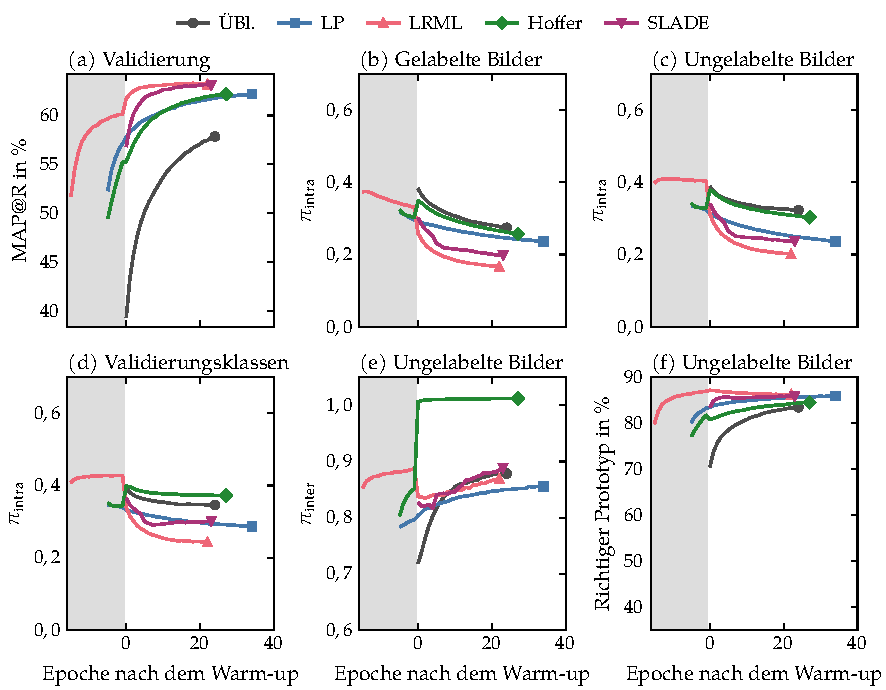
\includegraphics{neu/verlauf_k32}
  \caption[Trainingsverlauf bei 32 Labels je Klasse]{Validierungs-\acs{MAP@R} und Geometrie der Klassen über das Training bei $k=32$ (Cars196, Seed 2, Mittel über die fünf Verlustfunktionen und die vier Folds, ausgerichtet am Ende des Warm-ups). (a) Validierungs-\acs{MAP@R}, (b) bis (d) $\pi_{\mathrm{intra}}$ der gelabelten und der ungelabelten Bilder sowie der Validierungsklassen, (e) $\pi_{\mathrm{inter}}$, (f) Anteil der ungelabelten Bilder mit richtigem nächstem Klassenprototyp. Grau: Warm-up. Marker: Stopp des ersten Laufs.}
  \label{fig:a:verlauf32}
\end{figure}

\begin{figure}[tbp]
  \centering
  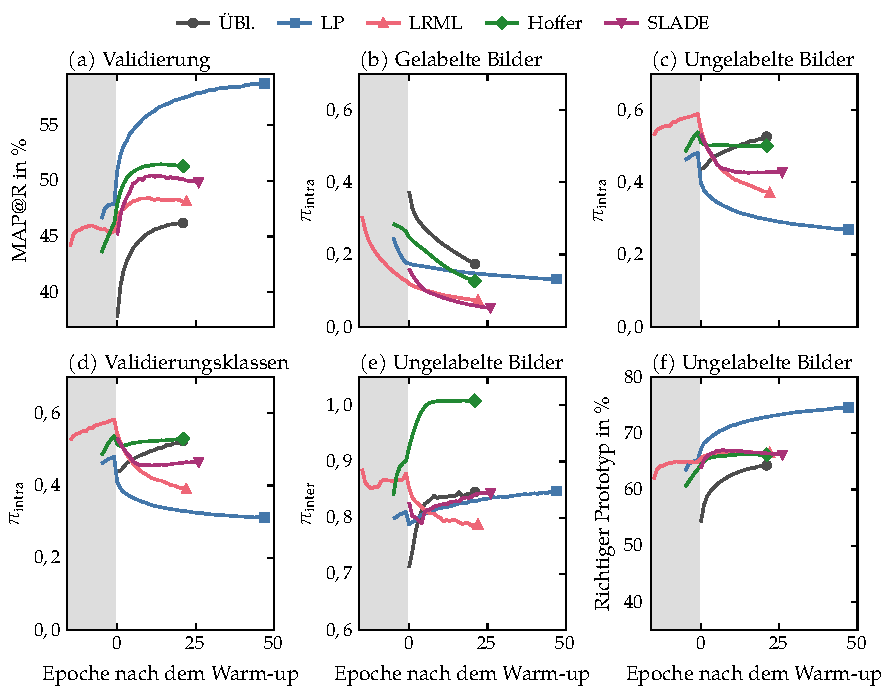
\includegraphics{neu/verlauf_k4}
  \caption[Trainingsverlauf bei vier Labels je Klasse]{Validierungs-\acs{MAP@R} und Geometrie der Klassen über das Training bei $k=4$, Teilabbildungen, Mittelung und Ausrichtung wie in Abbildung \ref{fig:a:verlauf32}.}
  \label{fig:a:verlauf4}
\end{figure}

\begin{figure}[tbp]
  \centering
  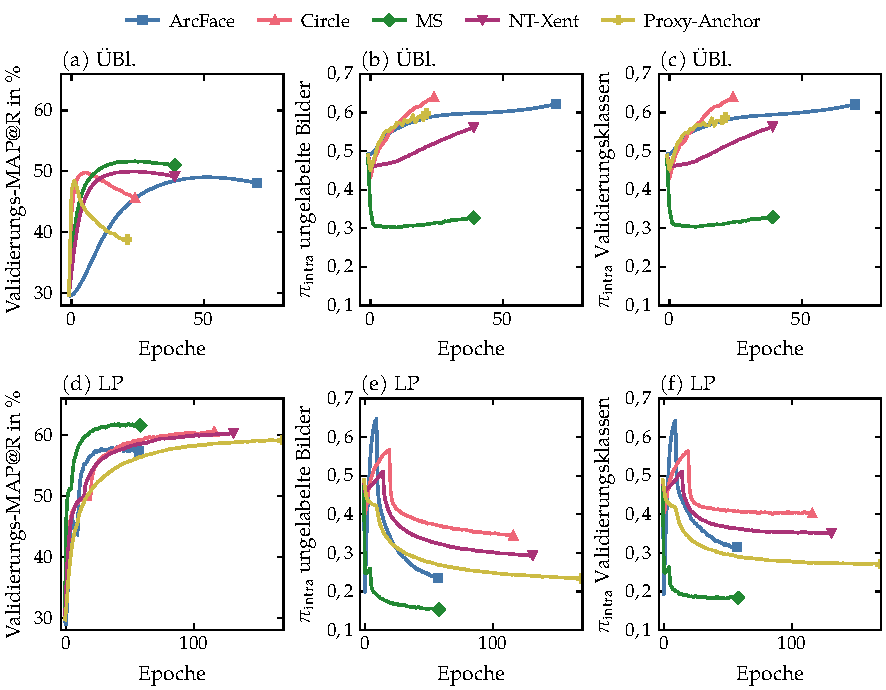
\includegraphics{neu/verlauf_verluste}
  \caption[Trainingsverlauf der \UEBL und von \acs{LP} mit allen Verlustfunktionen]{Validierungs-\acs{MAP@R} und $\pi_{\mathrm{intra}}$ der ungelabelten Bilder und der Validierungsklassen über das Training für die \UEBL (a bis c) und \acs{LP} (d bis f) bei $k=4$ mit allen fünf Verlustfunktionen (Cars196, Seed 2, Mittel über vier Folds, Marker am Kurvenende). Bei \acs{LP} mit ArcFace rückten bei Epoche 0 vorübergehend alle Bilder zusammen.}
  \label{fig:a:verluste}
\end{figure}

\begin{figure}[tbp]
  \centering
  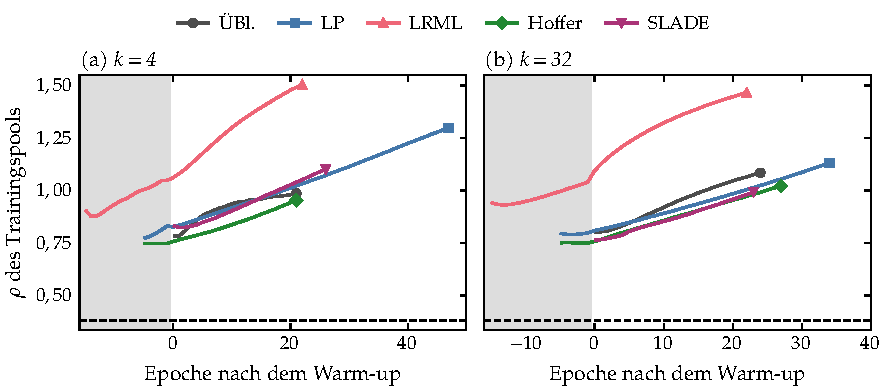
\includegraphics{neu/verlauf_rho}
  \caption[Spektraler Abfall über das Training]{Spektraler Abfall $\rho$ des Trainingspools über das Training bei (a) $k=4$ und (b) $k=32$ (Cars196, Seed 2, Mittel über die fünf Verlustfunktionen und die vier Folds, jeder Lauf am Ende seines Warm-ups ausgerichtet). Gestrichelt: DINOv2-Merkmale. Grau: Warm-up, gezeigt nur der allen Läufen gemeinsame Teil.}
  \label{fig:a:rho}
\end{figure}

\begin{figure}[tbp]
  \centering
  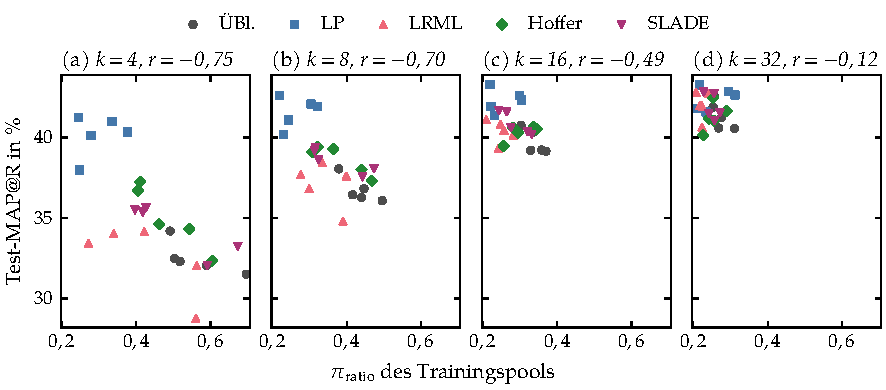
\includegraphics{neu/geometrie_korrelation}
  \caption[Geometrie und Retrieval-Leistung je Budget]{Test-\acs{MAP@R} der Einzelmodelle gegen $\pi_{\mathrm{ratio}}$ des Trainingspools nach dem Training für (a) $k=4$ bis (d) $k=32$, je Budget 25 Kombinationen aus Verfahren und Verlustfunktion (Cars196, Seed 2, Mittel über vier Folds). $r_{\mathrm{S}}$: Rangkorrelation nach Spearman innerhalb des Budgets.}
  \label{fig:e:geo:korrelation}
\end{figure}

\begin{table}[tbp]
\centering\small\setlength{\tabcolsep}{3.2pt}
\caption[Geometrie nach dem Training je Verlustfunktion]{$\pi_{\mathrm{intra}}$ der ungelabelten und, in Klammern, der gelabelten Bilder des Trainingspools und Test-MAP@R (Mean) nach dem Training je Verlustfunktion (Cars196, Seed 2, Mittel über vier Folds). Fett: kleinstes $\pi_{\mathrm{intra}}$ der ungelabelten Bilder und größte MAP@R je Zeile, bei gleichen gerundeten Werten nach dem ungerundeten Wert.}
\label{tab:a:geometrie}
\begin{tabular}{@{}l S[table-format=1.2] S[table-format=1.2] S[table-format=1.2] S[table-format=1.2] S[table-format=1.2] S[table-format=2.1] S[table-format=2.1] S[table-format=2.1] S[table-format=2.1] S[table-format=2.1]@{}}
\toprule
& \multicolumn{5}{c}{$\pi_{\mathrm{intra}}$ ungelabelt (gelabelt)} & \multicolumn{5}{c}{Test-MAP@R in \%} \\
\cmidrule(lr){2-6}\cmidrule(l){7-11}
{Verlust} & {\UEBL} & {LP} & {\acs{LRML}} & {Hoffer} & {SLADE} & {\UEBL} & {LP} & {\acs{LRML}} & {Hoffer} & {SLADE} \\
\midrule
\multicolumn{11}{@{}l}{\emph{$k=4$}} \\
ArcFace & 0.60 & \bfseries 0.26 & 0.57 & 0.56 & 0.60 & 32.1 & \bfseries 38.0 & 32.0 & 34.3 & 32.1 \\
 & {(0,16)} & {(0,07)} & {(0,08)} & {(0,16)} & {(0,05)} & & & & & \\
Circle & 0.52 & \bfseries 0.34 & 0.38 & 0.42 & 0.39 & 32.3 & \bfseries 41.0 & 34.1 & 36.7 & 35.7 \\
 & {(0,24)} & {(0,19)} & {(0,12)} & {(0,08)} & {(0,08)} & & & & & \\
MS & 0.31 & \bfseries 0.16 & 0.19 & 0.42 & 0.30 & 34.2 & \bfseries 41.3 & 33.4 & 37.3 & 35.5 \\
 & {(0,14)} & {(0,08)} & {(0,08)} & {(0,10)} & {(0,04)} & & & & & \\
NT-Xent & 0.51 & \bfseries 0.29 & 0.32 & 0.43 & 0.42 & 32.5 & \bfseries 40.1 & 34.0 & 34.6 & 35.4 \\
 & {(0,20)} & {(0,13)} & {(0,06)} & {(0,22)} & {(0,09)} & & & & & \\
Proxy-Anchor & 0.47 & \bfseries 0.23 & 0.27 & 0.62 & 0.40 & 31.5 & \bfseries 40.4 & 28.8 & 32.3 & 33.2 \\
 & {(0,11)} & {(0,12)} & {(0,03)} & {(0,20)} & {(0,10)} & & & & & \\
\addlinespace
\multicolumn{11}{@{}l}{\emph{$k=32$}} \\
ArcFace & 0.29 & \bfseries 0.21 & 0.25 & 0.32 & 0.30 & \bfseries 41.9 & 41.8 & 40.6 & 41.6 & 41.5 \\
 & {(0,20)} & {(0,21)} & {(0,18)} & {(0,25)} & {(0,23)} & & & & & \\
Circle & 0.35 & 0.31 & \bfseries 0.23 & 0.26 & 0.25 & 40.6 & 42.6 & 42.0 & 41.2 & \bfseries 42.7 \\
 & {(0,25)} & {(0,32)} & {(0,19)} & {(0,22)} & {(0,21)} & & & & & \\
MS & 0.21 & \bfseries 0.14 & 0.21 & 0.25 & 0.18 & 42.5 & \bfseries 43.3 & 42.7 & 40.1 & 42.8 \\
 & {(0,16)} & {(0,14)} & {(0,18)} & {(0,20)} & {(0,16)} & & & & & \\
NT-Xent & 0.30 & 0.23 & \bfseries 0.20 & 0.28 & 0.26 & 40.6 & 41.6 & \bfseries 42.8 & 41.1 & 41.5 \\
 & {(0,21)} & {(0,24)} & {(0,16)} & {(0,23)} & {(0,21)} & & & & & \\
Proxy-Anchor & 0.24 & 0.18 & \bfseries 0.18 & 0.29 & 0.22 & 41.2 & \bfseries 42.9 & 42.0 & 42.5 & 41.1 \\
 & {(0,17)} & {(0,19)} & {(0,13)} & {(0,20)} & {(0,17)} & & & & & \\
\bottomrule
\end{tabular}
\end{table}


\begin{table}[tbp]
\centering
\caption[Reinheit des $k$NN-Graphen von LRML]{Reinheit des $k$NN-Graphen von \acs{LRML} nach dem Training (Anteil der Kanten innerhalb einer Klasse in \%) mit der Nachbarzahl der Konfiguration der Geometrieläufe (Cars196, Seed~2, Mittel über vier Folds). Head ($-1$): vor dem ersten Optimierungsschritt. Nur innerhalb einer Zeile vergleichbar, weil sich die Nachbarzahlen unterscheiden.}
\label{tab:a:reinheit:lrml}
\begin{tabular}{@{}l S[table-format=2.0] S[table-format=2.1] S[table-format=2.1] S[table-format=2.1] S[table-format=2.1] S[table-format=2.1]@{}}
\toprule
{Verlust} & {Nachbarn} & {Head ($-1$)} & {$k=4$} & {$k=8$} & {$k=16$} & {$k=32$} \\
\midrule
ArcFace & 49 & 30.8 & 56.3 & 67.2 & 74.1 & 78.5 \\
Circle & 77 & 24.9 & 48.7 & 57.7 & 62.5 & 65.4 \\
\acs{MS} & 50 & 30.6 & 57.6 & 68.1 & 74.6 & 76.5 \\
NT-Xent & 52 & 30.1 & 58.1 & 68.1 & 73.7 & 76.6 \\
Proxy-Anchor & 25 & 39.4 & 62.1 & 74.5 & 82.2 & 85.2 \\
\bottomrule
\end{tabular}
\end{table}

\clearpage %
\begingroup\small\setstretch{1}\setlength{\tabcolsep}{4pt}
\begin{longtable}{@{}ll S[table-format=1.0] S[table-format=1.2] S[table-format=1.2] S[table-format=1.2] S[table-format=1.2] S[table-format=2.1] S[table-format=3.0] S[table-format=2.1]@{}}
\caption[Geometrie auf Semi-iNat-2021 und In-Shop für alle Budgets]{Geometrie nach dem Training für alle Budgets von Semi-iNat-2021, In-Shop und der In-Shop-Serie mit gelabelten Klassen (Seed 2, Mittel über die vier Folds und die Verlustfunktionen, die bei diesem Budget für alle Verfahren vollständig vorliegen, Anzahl: Zahl dieser Verlustfunktionen). $\pi^{\mathrm{U}}_{\mathrm{intra}}$: ungelabelte Bilder, $\pi^{\mathrm{V}}_{\mathrm{ratio}}$: Validierungsklassen, Prototyp: Anteil der ungelabelten Bilder mit richtigem nächstem Klassenprototyp in \%, übrige Spalten wie in Tabelle \ref{tab:e:geometrie}.}\label{tab:a:geometrie:weitere}\\
\toprule
{Budget} & {Modell} & {Anzahl} & {$\rho$} & {$\pi_{\mathrm{ratio}}$} & {$\pi^{\mathrm{U}}_{\mathrm{intra}}$} & {$\pi^{\mathrm{V}}_{\mathrm{ratio}}$} & {Prototyp} & {Epoche} & {MAP@R} \\
\midrule
\endfirsthead
\multicolumn{10}{@{}l}{\small Tabelle \thetable{} (Fortsetzung)}\\
\toprule
{Budget} & {Modell} & {Anzahl} & {$\rho$} & {$\pi_{\mathrm{ratio}}$} & {$\pi^{\mathrm{U}}_{\mathrm{intra}}$} & {$\pi^{\mathrm{V}}_{\mathrm{ratio}}$} & {Prototyp} & {Epoche} & {MAP@R} \\
\midrule
\endhead
\midrule
\multicolumn{10}{r@{}}{\emph{Fortsetzung auf der nächsten Seite}}\\
\endfoot
\bottomrule
\endlastfoot
\multicolumn{10}{@{}l}{\emph{Semi-iNat-2021}} \\
$k=2$ & \UEBL & 5 & 0.52 & 0.68 & 0.67 & 0.69 & 56.3 & 11 & 34.1 \\
 & LP &  & 0.60 & 0.62 & 0.58 & 0.66 & 62.0 & 31 & 34.6 \\
 & \acs{LRML} &  & 0.53 & 0.67 & 0.66 & 0.68 & 56.4 & 7 & 34.0 \\
 & Hoffer &  & 0.52 & 0.68 & 0.67 & 0.69 & 56.4 & 8 & 34.0 \\
 & SLADE &  & 0.52 & 0.69 & 0.66 & 0.70 & 56.4 & 11 & 34.0 \\
$k=4$ & \UEBL & 5 & 0.53 & 0.66 & 0.64 & 0.68 & 67.0 & 18 & 34.7 \\
 & LP &  & 0.60 & 0.61 & 0.56 & 0.66 & 71.0 & 39 & 35.3 \\
 & \acs{LRML} &  & 0.55 & 0.65 & 0.63 & 0.67 & 67.1 & 10 & 34.5 \\
 & Hoffer &  & 0.54 & 0.66 & 0.64 & 0.68 & 67.0 & 8 & 34.6 \\
 & SLADE &  & 0.53 & 0.65 & 0.63 & 0.68 & 67.1 & 15 & 34.6 \\
$k=16$ & \UEBL & 5 & 0.59 & 0.59 & 0.58 & 0.65 & 78.8 & 45 & 36.0 \\
 & LP &  & 0.64 & 0.57 & 0.53 & 0.65 & 79.6 & 57 & 36.4 \\
 & \acs{LRML} &  & 0.61 & 0.58 & 0.55 & 0.65 & 78.8 & 29 & 35.8 \\
 & Hoffer &  & 0.59 & 0.60 & 0.58 & 0.65 & 78.9 & 23 & 36.0 \\
 & SLADE &  & 0.58 & 0.57 & 0.57 & 0.63 & 78.9 & 50 & 36.0 \\
$k=100$ & \UEBL & 5 & 0.65 & 0.54 & 0.53 & 0.64 & 83.7 & 85 & 37.1 \\
 & LP &  & 0.64 & 0.57 & 0.52 & 0.65 & 81.7 & 59 & 36.2 \\
 & \acs{LRML} &  & 0.69 & 0.53 & 0.49 & 0.63 & 83.2 & 56 & 36.6 \\
 & Hoffer &  & 0.66 & 0.54 & 0.53 & 0.64 & 83.9 & 50 & 37.1 \\
 & SLADE &  & 0.65 & 0.51 & 0.51 & 0.59 & 83.2 & 104 & 36.8 \\
\addlinespace
\multicolumn{10}{@{}l}{\emph{In-Shop}} \\
$k=2$ & \UEBL & 5 & 1.28 & 0.32 & 0.31 & 0.36 & 71.9 & 203 & 54.8 \\
 & LP &  & 1.81 & 0.29 & 0.27 & 0.34 & 74.9 & 235 & 57.9 \\
 & \acs{LRML} &  & 2.04 & 0.27 & 0.20 & 0.32 & 73.4 & 133 & 56.4 \\
 & Hoffer &  & 2.09 & 0.27 & 0.31 & 0.32 & 74.1 & 152 & 57.9 \\
 & SLADE &  & 1.12 & 0.32 & 0.35 & 0.35 & 71.7 & 233 & 54.2 \\
$k=4$ & \UEBL & 5 & 1.73 & 0.23 & 0.26 & 0.28 & 76.9 & 396 & 59.3 \\
 & LP &  & 1.63 & 0.28 & 0.27 & 0.33 & 78.2 & 224 & 59.1 \\
 & \acs{LRML} &  & 2.01 & 0.23 & 0.20 & 0.27 & 76.8 & 146 & 58.9 \\
 & Hoffer &  & 2.26 & 0.24 & 0.28 & 0.28 & 75.2 & 180 & 59.1 \\
 & SLADE &  & 1.26 & 0.24 & 0.30 & 0.28 & 76.6 & 329 & 58.7 \\
\addlinespace
\multicolumn{10}{@{}l}{\emph{In-Shop-Serie mit gelabelten Klassen}} \\
\qty{5}{\percent} & \UEBL & 5 & 0.90 & 0.39 & 0.36 & 0.40 & {--} & 92 & 43.3 \\
 & LP &  & 1.28 & 0.37 & 0.25 & 0.38 & {--} & 43 & 41.8 \\
 & \acs{LRML} &  & 1.23 & 0.31 & 0.26 & 0.33 & {--} & 41 & 44.2 \\
 & Hoffer &  & 0.87 & 0.41 & 0.34 & 0.42 & {--} & 66 & 43.2 \\
 & SLADE &  & 0.86 & 0.42 & 0.26 & 0.44 & {--} & 75 & 43.4 \\
\qty{10}{\percent} & \UEBL & 5 & 1.03 & 0.36 & 0.35 & 0.38 & {--} & 168 & 48.1 \\
 & LP &  & 1.33 & 0.32 & 0.24 & 0.34 & {--} & 65 & 46.7 \\
 & \acs{LRML} &  & 1.44 & 0.26 & 0.24 & 0.28 & {--} & 78 & 49.2 \\
 & Hoffer &  & 1.00 & 0.39 & 0.33 & 0.41 & {--} & 130 & 47.9 \\
 & SLADE &  & 0.89 & 0.37 & 0.25 & 0.40 & {--} & 123 & 47.7 \\
\qty{25}{\percent} & \UEBL & 4 & 1.30 & 0.30 & 0.30 & 0.33 & {--} & 331 & 54.6 \\
 & LP &  & 1.37 & 0.27 & 0.19 & 0.29 & {--} & 112 & 51.0 \\
 & \acs{LRML} &  & 1.43 & 0.24 & 0.15 & 0.26 & {--} & 123 & 52.3 \\
 & Hoffer &  & 1.21 & 0.34 & 0.31 & 0.38 & {--} & 297 & 54.5 \\
 & SLADE &  & 0.95 & 0.30 & 0.22 & 0.32 & {--} & 161 & 52.2 \\
\qty{50}{\percent} & \UEBL & 3 & 1.48 & 0.26 & 0.30 & 0.30 & {--} & 306 & 57.8 \\
 & LP &  & 1.29 & 0.26 & 0.23 & 0.28 & {--} & 171 & 52.6 \\
 & \acs{LRML} &  & 1.66 & 0.22 & 0.16 & 0.25 & {--} & 298 & 56.2 \\
 & Hoffer &  & 1.32 & 0.27 & 0.31 & 0.31 & {--} & 353 & 58.0 \\
 & SLADE &  & 1.03 & 0.26 & 0.27 & 0.30 & {--} & 408 & 57.1 \\
\end{longtable}
\endgroup


\chapter{Verzögerte Patience}
\label{chap:anhang:verzoegerung}

Dieser Anhang ergänzt Abschnitt \ref{sec:training}. In manchen Folds brach die Validierungs-\ac{MAP@R} in der ersten Trainingsepoche stark ein, sodass ihr Höchstwert bereits vor dem Training lag. Derselbe Einbruch kann auch nach einem Warm-up auftreten. Anschließend stieg die Validierungs-\ac{MAP@R} zwar wieder an, aber so langsam, dass sie den Höchstwert nicht innerhalb der Patience übertraf und das Training abbrach. Als zu früh gilt ein Abbruch, wenn die beste Epoche vor der 20. Epoche nach dem Warm-up liegt (ohne Warm-up vor der 20. Trainingsepoche) und die Validierungs-\ac{MAP@R} bis zum Abbruch noch steigt. Als steigend gilt sie, wenn die Ausgleichsgerade durch ihre Werte der letzten zehn Epochen bis zum Abbruch eine positive Steigung hat. Mit verzögerter Patience verbrauchen die ersten 20 Epochen nach dem Warm-up, ohne Warm-up die ersten 20 Trainingsepochen, keine Patience. Danach zählt die Patience die Epochen, in denen die Validierungs-\ac{MAP@R} nicht über ihren höchsten Wert ab der letzten dieser Epochen steigt. Gewählt wird wie ohne Verzögerung das Modell der Epoche mit der besten Validierungs-\ac{MAP@R}.

Zu früh beendet wurden 541 Folds in 339 Läufen aus beiden Phasen, dem Versuch mit externen Bildern und den Geometrieläufen. Ausgenommen sind die Läufe auf \ac{CUB} mit ihrer Patience von 40 Epochen und die Versuche der Hyperparametersuche. Die Ablationen bei $k=8$ wurden für jeden Lauf mit Verzögerung trainiert (Abschnitt \ref{sec:m:phase2}).

Für die 321 Läufe mit einem zu früh beendeten Fold, für die die Arbeit die Variante ohne Verzögerung berichtet, zeigen Abbildung \ref{fig:a:verzoegerung} und Tabelle \ref{tab:anhang:verzoegerung} die Test-\ac{MAP@R} mit verzögerter Patience als zweiten Wert. Im Mittel änderte sie sich um \num{0.06} Prozentpunkte. Bis zum früheren Abbruch durchliefen beide Varianten in 313 Läufen dieselbe Validierungskurve. In 188 Läufen validierten sie gleich und wählten dieselbe Epoche, in 132 validierte die Variante mit Verzögerung besser. Die Differenz in der Validierung hängt mit der im Test zusammen (Korrelation \num{0.73}), sagt sie aber nur grob voraus. In 70 der 132 Läufe sank die Test-\ac{MAP@R}, vor allem mit externen Bildern auf Cars196. Dort validierte die Variante mit Verzögerung in 64 der 133 Läufe besser, die Test-\ac{MAP@R} sank aber in 58 davon, im Mittel um \num{0.8} Prozentpunkte. Die Validierung überschätzt dort also den Nutzen eines längeren Trainings. Am stärksten stieg die Test-\ac{MAP@R} in den Ablationen der Phase 2, um bis zu \num{7.2} Prozentpunkte bei \ac{LP} mit ArcFace und der Konfidenzschwelle \num{0.7} auf In-Shop. In den beiden Läufen mit den größten Einbrüchen der Sweeps von \ac{SLADE} (Abschnitt \ref{sec:e:sweeps}) beendete die Patience das Training in mehreren Folds zu früh. Mit verzögerter Patience verlor \ac{SLADE} beim kleinen Basis-Zielverhältnis \num{11.5} statt \num{16.6} und bei 512 ungelabelten Bildern je Batch \num{14.9} statt \num{20.5} Prozentpunkte.

Für die \UEBL mit Proxy-Anchor in der In-Shop-Serie mit gelabelten Klassen bei 10 bis \qty{50}{\percent} berichtet die Arbeit die Variante mit Verzögerung, in 15 Läufen und den drei zugehörigen Geometrieläufen. Ohne Verzögerung übertraf die Validierungs-\ac{MAP@R} dort in mindestens einem Fold innerhalb der Patience nie den Wert vor dem ersten Trainingsschritt. Ihre Test-\ac{MAP@R} läge dann bei \qty{13.3}{\percent} bis \qty{39.7}{\percent} statt \qty{48.0}{\percent} bis \qty{57.4}{\percent}, weil einzelne Folds den zufällig initialisierten Head wählten.

\begin{figure}[tbp]
  \centering
  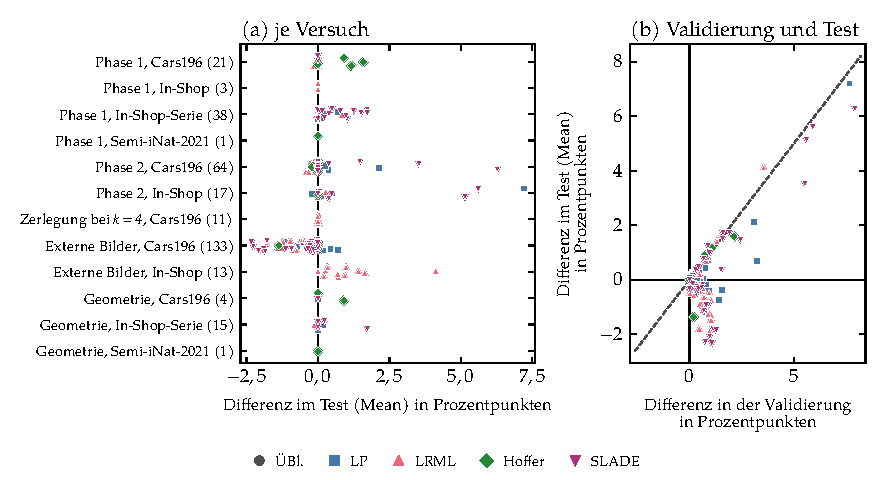
\includegraphics{neu/verzoegerung}
  \caption[Wirkung der verzögerten Patience je Lauf]{Test-\acs{MAP@R} der Einzelmodelle mit verzögerter Patience minus der ohne Verzögerung für die 321 Läufe mit einem zu früh beendeten Fold, (a) je Versuch mit der Zahl der Läufe, (b) gegen die Differenz der Validierungs-\acs{MAP@R}. Gestrichelt: gleiche Differenz in Validierung und Test. Ohne die 18 Läufe der \UEBL mit Proxy-Anchor in der In-Shop-Serie.}
  \label{fig:a:verzoegerung}
\end{figure}

\begin{table}[tbp]
\centering
\caption[Wirkung der verzögerten Patience]{Läufe mit einem zu früh beendeten Fold (Abschnitt \ref{sec:training}): Test-MAP@R mit verzögerter Patience minus der ohne Verzögerung in Prozentpunkten, Mittel und Spanne über die Läufe sowie die Zahl der Läufe, die mit Verzögerung besser validierten.}
\label{tab:anhang:verzoegerung}
\small
\begin{tabular}{@{}l S[table-format=3.0] S[table-format=-1.2] c S[table-format=-1.2] S[table-format=3.0]@{}}
\toprule
{Versuch} & {Läufe} & {Mean} & {\shortstack{Spanne\\(Mean)}} & {Concat} & {\shortstack{Validierung\\besser}} \\
\midrule
Phase 1, Cars196 & 21 & 0.17 & \num{-0.1} bis \num{1.6} & 0.12 & 4 \\
Phase 1, In-Shop & 3 & 0.00 & \num{0.0} bis \num{0.0} & 0.00 & 0 \\
Phase 1, In-Shop-Serie & 38 & 0.32 & \num{-0.1} bis \num{1.7} & 0.46 & 17 \\
Phase 1, Semi-iNat-2021 & 1 & 0.00 & \num{0.0} bis \num{0.0} & 0.00 & 0 \\
Phase 2, Cars196 & 64 & 0.20 & \num{-0.4} bis \num{6.3} & 0.23 & 16 \\
Phase 2, In-Shop & 17 & 1.15 & \num{-0.2} bis \num{7.2} & 1.61 & 11 \\
Zerlegung bei $k=4$, Cars196 & 11 & 0.01 & \num{0.0} bis \num{0.1} & 0.10 & 2 \\
Externe Bilder, Cars196 & 133 & -0.33 & \num{-2.3} bis \num{0.7} & 0.06 & 64 \\
Externe Bilder, In-Shop & 13 & 0.89 & \num{0.0} bis \num{4.1} & 0.86 & 11 \\
Geometrie, Cars196 & 4 & 0.23 & \num{0.0} bis \num{0.9} & 0.12 & 1 \\
Geometrie, In-Shop-Serie & 15 & 0.15 & \num{-0.1} bis \num{1.7} & 0.25 & 6 \\
Geometrie, Semi-iNat-2021 & 1 & 0.00 & \num{0.0} bis \num{0.0} & 0.00 & 0 \\
\midrule
alle & 321 & 0.06 & \num{-2.3} bis \num{7.2} & 0.27 & 132 \\
\bottomrule
\end{tabular}
\end{table}

